% This is a sample thesis file for CPP Math Grad Students to follow.
% After downloading this file to your computer, save it with whatever name you wish.
% Also download the file CPP.cls and save it in the same folder as this file.
% Do not change the name of the file CPP.cls.
\documentclass{CPP}

% Include packages
\usepackage{amsmath}             % Provides various math environments
\usepackage{amssymb}             % Provides various math symbols
\usepackage{amsthm}
% Provides theorem environments
\usepackage{graphicx}            % Provides ability to include images
\usepackage[page]{appendix}      % Provides appendices environment
\usepackage{float}
\usepackage[colorlinks=True, allcolors=black]{hyperref}
\usepackage{url}
\usepackage[table, dvipsnames]{xcolor}
\definecolor{lightgray}{gray}{.7}
\usepackage{booktabs, xltabular, longtable}  % For tables
\newcolumntype{P}[1]{>{\centering\arraybackslash}p{#1}}
\usepackage{siunitx}
\usepackage{color, colortbl}
\usepackage{systeme}
\usepackage{bm}
\usepackage{listings}
\usepackage{ragged2e}
% \usepackage{setspace}

\usepackage{tablefootnote}


% ============================================================================= %
  
\begin{document}

% Enter the information indicated inside the curly brackets below
\titleone{Alaskan Brown Bears and Pacific Salmon}
\titletwo{Face the Effects of Global Warming}
\titlethree{}
\doctype{Thesis}
\doctypeUp{Thesis}
\degree{Master of Science}
\field{Mathematics}
\Author{Connor Adams}
\Advisor{Hubertus Von Bremen}
\MemberA{Berit Givens}
\MemberB{Jennifer Switkes}
\Year{2022}
\Semester{Fall}

% Type your abstract inside the curly brackets below
\Abstract{Climate change has been a popular topic since James Hansen gave his testimony to Congress in 1988, expressing the disasters that would come from global warming.
Many researchers are studying climate change in hopes of predicting its effects.
If we can anticipate the outcomes of climate change, we can take measures to minimize or eliminate the catastrophes that will follow.
In this thesis, we compare two models that determine the long-term outcome of two interactive species, pacific salmon \emph{Oncorhynchus} and Alaskan brown bears \emph{Ursus arctos}.
The first model predicts the outcome of the species when temperature is constant, and the other when temperature is a function of time.
We conclude that the effects of global warming could cause the pacific salmon to either die off or migrate to an area that is more suitable for their environmental needs, resulting in the brown bear population decreasing in size to accommodate for the elimination of a food source.}

% Type your acknowledgments inside the curly brackets below
\Acknowledgments{First, I would like to thank my advisor, Dr. Hubertus Von Bremen, who guided my thinking and patiently assisted me throughout my graduate program.
I greatly appreciate you pushing me to learn and explore more mathematical ideas during this amazing process.
Because of you, I aim to further my education in applied mathematics as well as computer programming.

I also want to thank my family for supporting me through many sleepless days.
More specifically, I want to thank my mom and dad for helping me stay focused and determined every day.
Furthermore, I am grateful for my fianc\'{e}e, who has sacrificed her time and education for me.
I am excited to return the favor by helping you get your master's degree.

My gratitude goes out to all my close friends and colleagues, Joshua Garcia, Nick Beltz, Ethan Flora, Daniel Silva, Jeffrey Robbins, Seth Ricarte, Jose Contreras, Sara Elakesh, Michael Yates, and Latimer De'Shone Harris-Ward, for all your encouragement and mathematical aid that has made this possible.

I would also like to thank Dr. Berit Givens, Dr. John Rock, and Dr. Jennifer Switkes, who have had the most significant impact on my thinking as a mathematician.
I appreciate your guidance and dedication to helping me understand and apply mathematical concepts.
You all have inspired me to become a better mathematician, and I will always aim to be as knowledgeable as you all.

Lastly, I want to extend my gratitude to Aaron Tiernan, an Area Management Biologist for the ADFG. Thank you for helping me gather information about the salmon population in Bristol Bay.
}

% The following generates a title page, a signature page, an acknowledgments 
% page, an abstract page, and a table of contents
\titlepage
\signaturepage{\addcontentsline{toc}{chapter}{Signature Page}}
\acknowledgmentspage{\addcontentsline{toc}{chapter}{Acknowledgements}}
\abstractpage{\addcontentsline{toc}{chapter}{Abstract}}
\tableofcontents

% Comment out either or both of the following two lines to remove
% the List of Figures and/or List of Tables, as is appropriate for your thesis
\listoftables{\addcontentsline{toc}{chapter}{List of Tables}}
\listoffigures{\addcontentsline{toc}{chapter}{List of Figures}}

% Reset the page counter for the main body of the thesis
\newpage
\pagenumbering{arabic} \setcounter{page}{1} \thispagestyle{empty}

% The \AddChap command should be issued before the first chapter to update
% the display style in the Table of Contents
\AddChap

% ----------------------------------------------------------------------------- %

% Change the titles of Chapters and Sections below as desired.

% ----------------------------------------------------------------------------- %
\chapter{Introduction}

The topic of climate change has been debated for many years, with some people believing that global warming is a myth and misusing scientific research to support their claims~\cite{allchin2015global}.
% Since the beginning of the 20$^{th}$ century, global temperatures have been increasing on average, with little to no evidence of stopping~\cite{NOAA}.
Many researchers have concluded that the earth's temperature has increased significantly since the early 20$^\text{th}$ century and will continue to increase until at least the mid to late 21$^\text{st}$ century~\cite{hansen2006global,raftery2017less,osterkamp1990thermal}.
A group of researchers implemented a joint Bayesian hierarchical model, which determined that global temperatures will likely increase by an average of $3.2^{\circ}$C entering the 22$^\text{nd}$ century~\cite{raftery2017less}.
% which sparked the creation of a new lifestyle \cite{crowley2000causes}.
When the industrial revolution began, a significant amount of greenhouse gases, such as carbon dioxide, methane, nitrous oxide, and fluorinated gases, filled our atmosphere, acting as a canopy that prevents heat from escaping the atmosphere, thus causing an escalation in climate temperature~\cite{crowley2000causes, osterkamp1990thermal, epagreen}.
In 2019, the EPA reported that 80\% of the earth's greenhouse gases are carbon dioxide~\cite{epagreen}.
Because of the high demand for transportation, electricity, industrial production, and residential/commercial use of fossil fuels, carbon dioxide will continue to be the primary cause of greenhouse gas emissions~\cite{epagreen}.
% Trees, plants, and the ocean are part of the carbon cycle, which removes massive amounts of carbon dioxide from the atmosphere.
% Carbon dioxide emissions have been declining slowly over the past 15 years, so global temperature trends may decrease in the near future~\cite{epagreen}.
Now realizing the damage we have done to the earth, we are trying to resolve the problem without sacrificing our comfort. 
Unfortunately, this realization is too late for some species, such as the polar and koala bears~\cite{adams2011modelling,wiig2008effects, stirling2012effects}.
In this thesis, we investigate the effects of climate change on a pair of species known to interact with each other, pacific salmon \emph{Oncorhynchus} and Alaskan brown bears \emph{Ursus arctos}.
% In this thesis, we review various nonlinear differential equation models while implementing the Lotka-Volterra equations to simulate the effects of climate change on interactive species such as; brown bears with salmon.
% Nonlinear differential equations will be used to model species that follow logistic growth pattern. An inspiration of the Lotka-Volterra equation is used in representing the interaction between two species.
% The primary focus of this work is to display the effects of climate change and illustrate the potential dangers that may lie ahead if a solution isn't discovered.
% Currently, some sea life animals are starting to experience the side effects of global warming.
% One species in particular facing the effects of sea temperature change are pacific salmon \emph{Oncorhynchus}.

Pacific salmon are sensitive to their environment and rely on sufficient river temperatures to survive spawning migration~\cite{ADFG}.
Adult salmon live in the ocean, but when the time comes to reproduce, they swim up river streams to lay their eggs and usually die shortly after; this is referred to as spawning. 
Salmon like to begin their journey from salt water to fresh water between late spring and early summer, but this depends on the species and location of pacific salmon \cite{ADFG}.
Specifically in Alaska, salmon can be seen spawning in river streams between the middle of July through late October \cite{lisi2013association}.
As river temperatures rise, the months in which they spawn and where they spawn may change, respectively~\cite{taylor2008climate}.
Thus, global warming could affect the population of pacific salmon as well as any species that interact with them. 
% This doesn't seem like a big deal since in theory their spawning time will just change \cite{ADFG}. 
% Well, Alaskan brown bears feed off salmon during this time and this is a large portion of their diet.

Alaskan brown bears feed on salmon as they migrate upstream, and if the population of salmon is susceptible to changes in temperature, then the brown bears could also be affected.
Bears hibernate during winter and emerge during spring. 
Once emerged, they consume an enormous amount of food, such as berries, roots of plants, squirrels, moose, caribou, and fish~\cite{ADFG}.
Alaskan brown bears have various food sources, but salmon is an essential part of their diet, consuming an average of 1099 kg per year~\cite{deacy2018phenological,hilderbrand1999effect}. 
% If the change in sea temperature directly effects the lives of salmon, then we can expect to see the lives of those that depend on that food source to be negatively effected, like brown bears.
Pacific salmon are already migrating further north, where temperatures are more suitable for them~\cite{taylor2008climate}.
Since salmon is an essential food source for brown bears, it is probable that the species will either migrate with the salmon or look for another abundant resource to feed on~\cite{hilderbrand1999effect}.
% So, some of these side effects consist of the migration of salmon to temperatures that better suit them; therefore resulting in the possible migration of brown bears, replacement of salmon as a food source, or even a reduction in population if unable to compensate in the loss of a food source. In order for the brown bear population to live on, they will need to eventually adapt to this new environment they are approaching.

%%%%%%%%%%%%%%%%%%%%%%%%%%%%%%%%%%%%%%%%%%%%%%

%%%%%%%%%%%%%%%%%%%%%%%%%%%%%%%%%%%%%%%%%%%%%%

% % Chapter 2
% In chapter 2, we provide background information on the effects of global warming as well as the causes for the increase in the earth's climate temperature since the early 20$^{th}$ century.
% We also briefly mention global temperature predictions for the next hundred years.
% For the remaining sections of the chapter, we review population and interaction models, such as exponential growth, logistic growth, and Lotka-Volterra equations, which we use to construct our models.
% Lastly, we finish the chapter by reviewing Theodore Modis' competitive predator-prey model, which we use in chapter 5 to introduce an interaction between the species.

%%%%%%%%%%%%%%%%%%%%%%%%%%%%%%%%%%%%%%%%%%%%%%

%%%%%%%%%%%%%%%%%%%%%%%%%%%%%%%%%%%%%%%%%%%%%%

% Chapter 2
In chapter 2, we use the logistic growth equation to model the population growth of pacific salmon and Alaskan brown bears.
We begin by estimating the growth rate parameter for salmon using the reproduction rate from the Western Fisheries Research Center (WFRC) and the proportion of escapement from the National Park Service (NPS).
Then, using data from the 2021 Bristol Bay annual management report, we calculate the carrying capacity by determining the maximum volume of salmon for any given run.
Next, we compare growth rates from 3 different articles and calculate their average to approximate our growth rate for the brown bear model.
Lastly, we pick a carrying capacity for the brown bears using information published by the Alaskan Department of Fish and Game (ADFG).


% Chapter 3 begins the model creation processes by constructing differential equations that illustrates the population of the brown bears, as well as the pacific salmon species in Alaska. 
% Next, to incorporate the influence of temperature on salmon, a reproductive rate function is designed to reflect the change in reproduction depending on temperature. 
% This chapter concludes with a final function that models water temperature change in Alaskan rivers and streams for the past 20 years.

%%%%%%%%%%%%%%%%%%%%%%%%%%%%%%%%%%%%%%%%%%%%%%

%%%%%%%%%%%%%%%%%%%%%%%%%%%%%%%%%%%%%%%%%%%%%%

% Chapter 3
In Chapter 3, we propose a salmon growth rate function dependent on time, which replaces the growth rate parameter in the salmon logistic model.
We use articles by Dr. Phyllis Weber Scannell and Katherine Carter to model the proportion of salmon that survive spawning migration at different temperatures.
Applying linear regression to 30 years of recorded Alaskan river data, we create a function to represent the change in Alaskan river temperature over time.
With this temperature function, we redesign the survival proportion model as a function of time.
Now, we construct the proposed salmon growth rate function by combining the growth rate parameter with the survival proportion function.
Finally, the growth rate function, $G(t)$, replaces the growth rate parameter in the salmon logistic model, creating a non-autonomous model for the salmon species.
% Chapter 4 continues the model creation process by combining the individual functions and equations in chapter 3 to construct a model that demonstrates the outcome of the salmon and brown bear species over time.

%%%%%%%%%%%%%%%%%%%%%%%%%%%%%%%%%%%%%%%%%%%%%%

%%%%%%%%%%%%%%%%%%%%%%%%%%%%%%%%%%%%%%%%%%%%%%

% Chapter 4
In Chapter 4, we begin by constructing a variation of Theodore Modis' model to introduce interaction between Alaskan brown bears and pacific salmon when neither species is affected by climate change.
We then solve for the critical points of our model and determine their stability by finding the eigenvalues of the Jacobian matrix.
% We then evaluate our model's stability by finding the eigenvalues of the Jacobian matrix for each critical point.
We explore different interaction parameters and visualize their effect by comparing the plots of our model's solutions for each pair of parameters.
Next, we fix the interaction parameters to $c_{xy} = 0.0627$, and $c_{yx} = 0.0313$, then plot each species population with respect to time.
We determine that the brown bear population will surpass the salmon population before both species oscillate toward their critical point, $(x=0.79,\;y=7.1)$.
Following this section, we introduce climate change into our model, letting the function, $G(t)$, represent the growth rate of salmon.
We then plot the solutions of the model using different initial conditions.
% We test different initial conditions and evaluate the stability of the model.
To compare the effects of climate change, we plot the solutions to this model with respect to time on top of the previous model's plot and denote the differences.
Lastly, we find that global warming causes the salmon species in Alaska to become regionally extinct, and in response to a diminished food resource, the brown bear species decrease in size relative to their population without the influence of climate change.
% Using the autonomous system of ODEs, we establish values for the interaction terms by deducing a criterion for the pair of parameters, then selecting a few from the criteria to analyze their effects on the model.
% Lastly, we compare the solutions to the autonomous and non-autonomous models.

%%%%%%%%%%%%%%%%%%%%%%%%%%%%%%%%%%%%%%%%%%%%%%

%%%%%%%%%%%%%%%%%%%%%%%%%%%%%%%%%%%%%%%%%%%%%%

% The purpose of this paper is to examine how the changing of the earth's temperature could affect the population of animals whose food source is relatively sensitive to environmental temperature, such as brown bears and salmon. 
% We will be using a modified predator-prey model that represents the population of Alaskan brown bears and salmon, which demonstrates the effects of climate change on both species.
% Ideally, this model could be applied to other interacting species that fall under similar conditions.
% For example, species that are strongly dependent on agriculture as a food source.
% Hopefully, this model will be used as a tool for scientists that assists in predicting the population of a species, which could influence government decisions on harvest rates, assist in determining the best place to relocate a species, or even design future models that would aid in predicting migration patterns of species that rely on similar parameters.

% ----------------------------------------------------------------------------- %

% \chapter{Background}

% \section{Climate Change}

% % The topic of climate change has been debated for many years. 
% Some people believe that global warming is a myth and misuse scientific research to support their claims~\cite{allchin2015global}. 
% % Thomas Crowley constructed a model using recorded weather data to determine temperature values up to 1000 years ago~\cite{crowley2000causes}.
% Many researchers have concluded that the earth's temperature has increased significantly since the early 20$^{th}$ century and will continue to increase until at least the mid to late 21$^{st}$ century~\cite{hansen2006global,raftery2017less,osterkamp1990thermal}.
% A group of researchers implemented a joint Bayesian hierarchical model, which determined that the global temperature will likely increase by an average of $3.2^{\circ}$C entering the 22$^{nd}$ century~\cite{raftery2017less}.
% This significant growth in temperature is due to the increase in greenhouse gases, such as carbon dioxide, methane, nitrous oxide, and fluorinated gases \cite{crowley2000causes, osterkamp1990thermal, epagreen}.
% Greenhouse gases fill the air and act as a canopy that prevents heat from escaping the atmosphere, causing an escalation in climate temperature~\cite{epagreen}. 
% In 2019, the EPA reported that 80\% of the earth's greenhouse gases are carbon dioxide~\cite{epagreen}.
% Because of the high demand for transportation, electricity, industrial production, and residential/commercial use of fossil fuels, carbon dioxide will continue to be the primary source of greenhouse gas emissions~\cite{epagreen}.
% Trees, plants, and the ocean are part of the carbon cycle, which removes massive amounts of carbon dioxide from the atmosphere.
% Carbon dioxide emissions have been declining slowly over the past 15 years, so global temperature trends may decrease in the near future~\cite{epagreen}.

% % The effects that will follow this dramatic temperature change will raise the average sea level, cause animals to migrate to new locations, threaten the population of animals that are sensitive to their climate conditions ~\cite{osterkamp1990thermal,adams2011modelling,taylor2008climate}

% % Global warming becomes more serious as the years keep rolling by. The most recent wake up calls are the effects on polar and koala bears \cite{wiig2008effects, adams2011modelling, stirling2012effects}. The permafrost in Alaska is melting which is causing damage to people's homes, roads, and pipelines
% % \cite{osterkamp1990thermal}. The population of polar bears are in a decline due to the melting of ice caps \cite{hunter2010climate}.
% % The koala bears in Australia had to migrate to new locations due to the increase in wildfires~\cite{adams2011modelling}.
% % These are just a few significant events that are breaking out in the world due to global warming, but we can expect to see more as time goes on.
% % Animals that are sensitive to their environment, such as many sea life, are under threat because the sea surface temperature is changing alongside the air temperature \cite{taylor2008climate,hansen2010global,iz2018global}.
% % For example, Salmon in Alaska are experiencing higher rates of prespawning mortality because they are migrating to the creeks earlier due to the shift in their environmental temperatures \cite{bowerman2018prespawn}. 
% % If the temperatures continue to increase, then prespawning mortality will increase as well \cite{bowerman2018prespawn}.
% % Scientists around the world have researched the causes for the sudden climb in temperature in hopes to find a solution to reverse the effects \cite{epagreen,cook2016consensus}.


% \section{Logistic Growth Model}

% % A simple equation for modeling population growth is the exponential ordinary differential equation (ODE), displayed below~\cite{tsoularis2002analysis},
% \begin{equation}\label{eq:expgrowthODE}
%     \frac{dx}{dt} = rx, \quad \text{where}\quad x(0) = x_0.
% \end{equation}
% Consider $r= \text{Birth} - \text{Death}>0$, then $r$ is a constant representing the growth rate of the population at any given time.
% Also, $x$ is the population at time $t$, so $\displaystyle \frac{dx}{dt}$ is the population rate of change that is dependent on $t$.
% As $t$ increases to infinity, the population, $x$, will also approach infinity due to the growth being exponential.
% So, a more accurate way to describe population growth is using a logistic growth ODE, which is given below~\cite{tsoularis2002analysis},
% \begin{equation}\label{eq:logisticgrowthODE}
%     \frac{dx}{dt} = rx\left(1-\frac{x}{K}\right).
% \end{equation}
% Here, $r$ still represents the growth rate of the population, and $K$ serves as the carrying capacity.
% Most species follow a logistic growth pattern due to environmental constraints, such as location, food, and other essential resources. 
% A great way to visualize $K$ as a carrying capacity is by graphing the right-hand side of~\equationautorefname \eqref{eq:logisticgrowthODE} as a function of $x$.
% \begin{figure}[H]
%     \centering
%     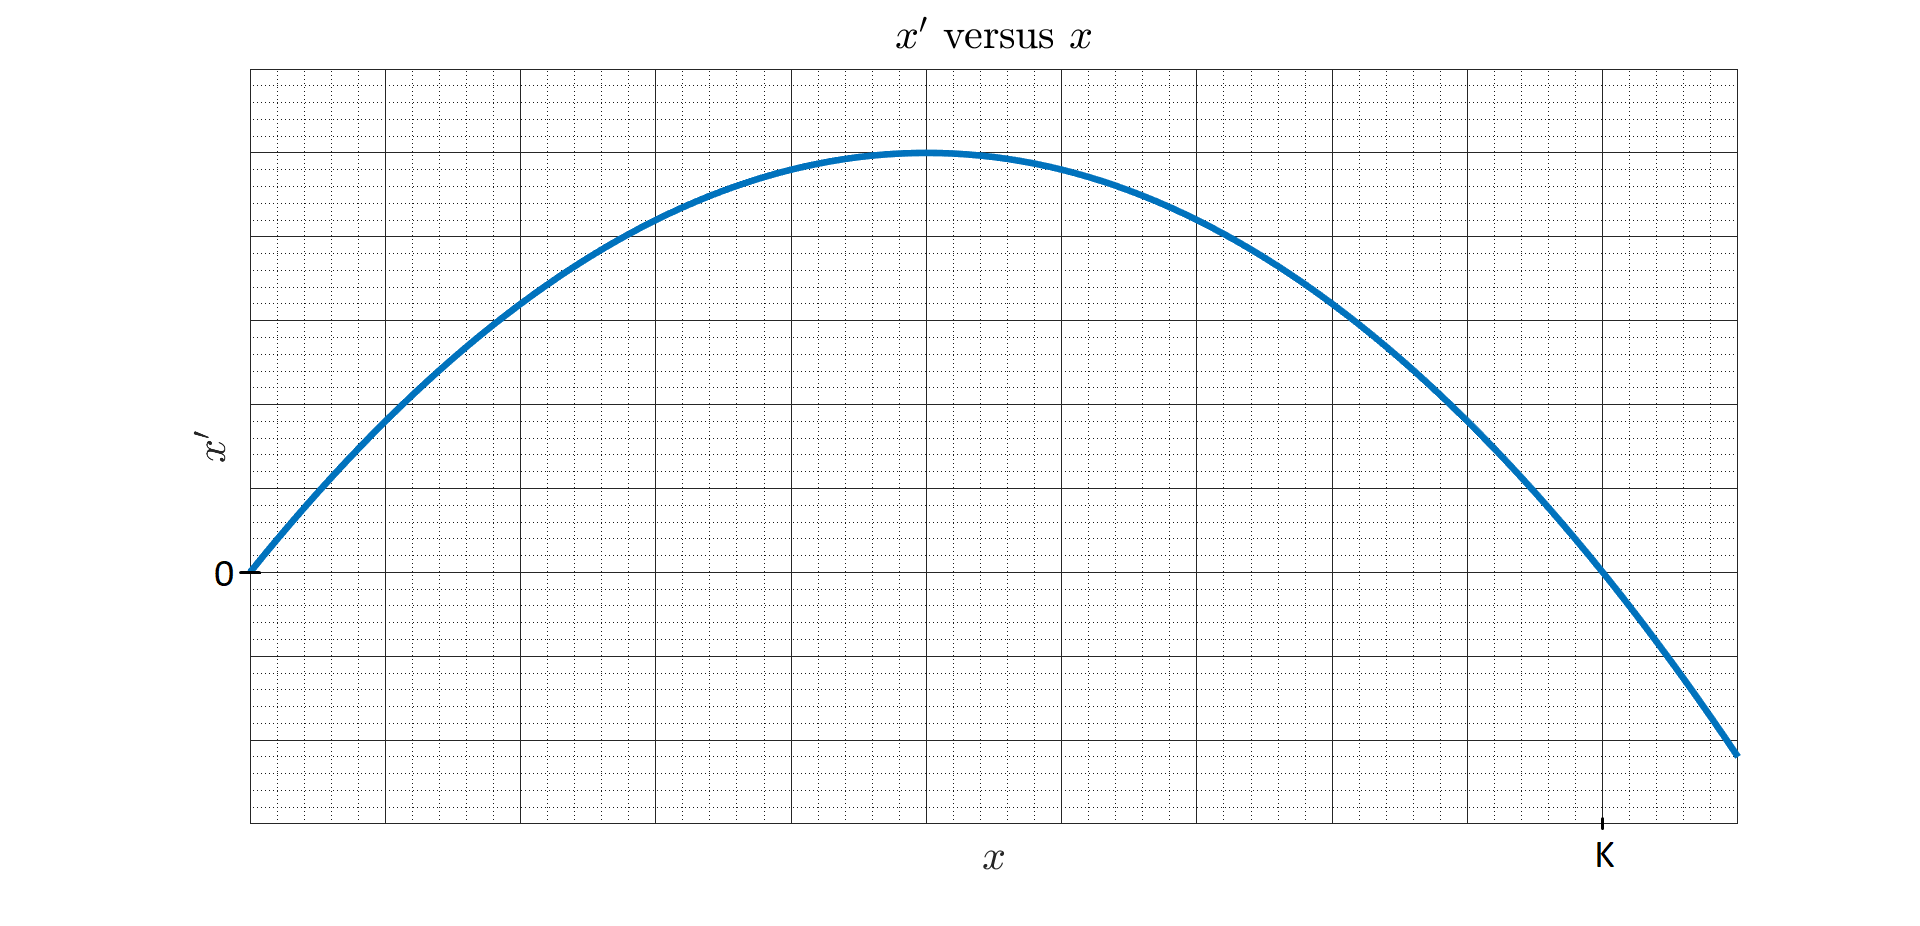
\includegraphics[width=14cm]{Pictures/ODE/LogODE.png}
%     \caption{Plot of the logistic growth equation as a function of $x$.}
%     \label{fig:logisticgrowthODE}
% \end{figure}
% The figure above illustrates that the population, $x$, will continue to grow when $x<K$, but decrease when $x>K$. The population will always be converging towards $K$, which is what we would expect to see in the real world. Thus, the logistic model is a more accurate representation of a specie's population.

% % by using the Lotka-Volterra equation an interaction between two species can be modeled.

% \section{Lotka-Volterra Model}

% % In nature, most animals share their environment, which sometimes causes species to interact, like salmon and brown bears. 
% This relationship can be portrayed by incorporating interaction terms into each species' population equation.
% The interaction terms depend on both species’ populations and use positive real parameters to describe the effect of one species on the other.
% The Lotka-Volterra model, also referred to as the predator-prey model, is a simple system of two nonlinear ordinary differential equations that utilize interaction terms to imitate the relationship between two species, displayed below~\cite{anisiu2014lotka},
% \begin{equation}\label{eq:lotkavoltera}
%     \begin{aligned}
%         \frac{dx}{dt} & = \alpha x - \beta xy,\\
%         \frac{dy}{dt} & = \delta xy - \gamma y.
%     \end{aligned}
% \end{equation}
% Consider $x$ as the prey, $y$ as the predator, and $\alpha$, $\beta$, $\delta$, $\gamma$ are positive real parameters that describe the interaction of the two species. 
% Also, $\displaystyle \frac{dx}{dt}$ and $\displaystyle \frac{dy}{dt}$ represent each species' instantaneous population rate of change. 
% The interaction term for species $x$ is subtracted from the exponential growth component, $\alpha x$, to describe that the instantaneous growth rate of species $x$ will decrease as $y$ increases. The opposite effect happens to species $y$ because the interaction term for species $y$ is added instead of subtracted.
% The author of ``US Nobel laureates: Logistic growth versus Volterra–Lotka'', Theodore Modis, developed a competitive predator-prey model that implements logistic growth instead of exponential, which is given below,
% \begin{equation}\label{eq:modislotkavoltera}
%     \begin{aligned}
%     \frac{dx}{dt} &= a_xx - b_xx^2 + c_{xy}xy,\\
%     \frac{dy}{dt} &= a_yy - b_yy^2 + c_{yx}xy,
%     \end{aligned}
% \end{equation}
% where $a_{x}$, $a_{y}$, $b_{x}$, $b_{y}$, $c_{xy}$ and $c_{yx}$ are positive real parameters that describe the interaction of the two species~\cite{modis2011us}.



% % This model is describing two species who have an interaction with themselves, which is the logistic equation, and an interaction with each other, which is the interaction terms added at the end of each equation.

% % The fundamentals of each of these equations will be used in the construction of our model. 
% % The Lotka-Volterra will assist in the illustrating interaction between species while the logistic equations will be used to describe the environmental limits of each species.




% \section{Trace-Determinant Plane}

% % The Trace-Determinant Plane is used to determine the  the stability of a system of ordinary differential equations like the Lotka-Voltera equation, \equationautorefname~\eqref{eq:lotkavoltera}, which can be rewritten in the following form.
% \begin{equation}\label{eq:lotkavoltera}
%     \begin{aligned}
%         f_x & = \alpha x - \beta xy\\
%         f_y & = \delta xy - \gamma y
%     \end{aligned}
% \end{equation}
% Then, a linearization of the above equation using the partial derivatives will produce the Jacobian matrix displayed below.
% \begin{equation}
%     J_{(x,y)}
% \end{equation}


% \begin{equation}
%     \begin{pmatrix}
%         x^'\\
%         y^'
%     \end{pmatrix}
%     =
%     \begin{pmatrix}
%         \alpha & -\beta x\\
%         \delta y & - \gamma
%     \end{pmatrix}
%     \begin{pmatrix}
%         x\\
%         y
%     \end{pmatrix}
% \end{equation}


% ----------------------------------------------------------------------------- %

\chapter{Logistic Models For The Species}

% Many population growth models use variations of the Verhulst logistic growth equation to simulate the population growth of living organisms.
% James Wallace and Anastasios Tsoularis review different variations of the logistic growth equation in their article, ``Analysis of logistic growth models''~\cite{tsoularis2002analysis}.
% In this thesis, we will use variations of the logistic growth model to describe the populations of pacific salmon and Alaskan brown bears.

In this chapter, we introduce simple logistic growth models for the salmon and brown bear species.
Using information from the Alaskan Department of Fish and Game, we estimate a growth rate parameter for the salmon population.
Then, we choose the carrying capacity parameter by calculating the maximum volume of salmon for any given inshore run\footnote{Inshore runs are when salmon migrate back from the sea to spawn.} in Bristol Bay, Alaska.
We find 3 growth rates from 3 articles for the Alaskan brown bears and calculate their mean, which we use to represent their growth rate parameter~\cite{daele2010management,mclellan1989,mclellan1996}.
Also, for this model, we estimate the carrying capacity based on information from the Alaskan Department of Fish and Game (ADFG)~\cite{ADFG}.



% we begin by creating an appropriate logistic growth model for the brown bear population using growth rates from a few scholarly articles and approximating a carrying capacity from the Alaskan Department of Fish and Game (ADFG). 
% Next, Volhulst’s logistic growth model will illustrate the salmon population using information from the ADFG to achieve a growth rate. 
% Also, the carrying capacity is revealed through the relationship between salmon run size and their average weight during their run. 
% Finally, the chapter briefly compares the two models and introduces the concept of creating a variation of the logistic model that incorporates the aspect of climate change.

% \section{Logistic Models}

% % % A simple equation for modeling population growth is the exponential ordinary differential equation (ODE), displayed below~\cite{tsoularis2002analysis},
% % \begin{equation}\label{eq:expgrowthODE}
% %     \frac{dx}{dt} = rx, \quad \text{where}\quad x(0) = x_0.
% % \end{equation}
% % Consider $r= \text{Birth} - \text{Death}>0$, then $r$ is a constant representing the growth rate of the population at any given time.
% % Also, $x$ is the population at time $t$, so $\displaystyle \frac{dx}{dt}$ is the population rate of change that is dependent on $t$.
% % As $t$ increases to infinity, the population, $x$, will also approach infinity due to the growth being exponential.
% So, a more accurate way to describe population growth is using a logistic growth ODE~\cite{tsoularis2002analysis},
% \begin{equation}\label{eq:logisticgrowthODE}
%     \frac{dx}{dt} = rx\left(1-\frac{x}{K}\right).
% \end{equation}
% Here, $r$ still represents the growth rate of the population, and $K$ serves as the carrying capacity.
% Most species follow a logistic growth pattern due to environmental constraints, such as location, food, and other essential resources. 
% A great way to visualize $K$ as a carrying capacity is by graphing the right-hand side of~\equationautorefname \eqref{eq:logisticgrowthODE} as a function of $x$.
% \begin{figure}[H]
%     \centering
%     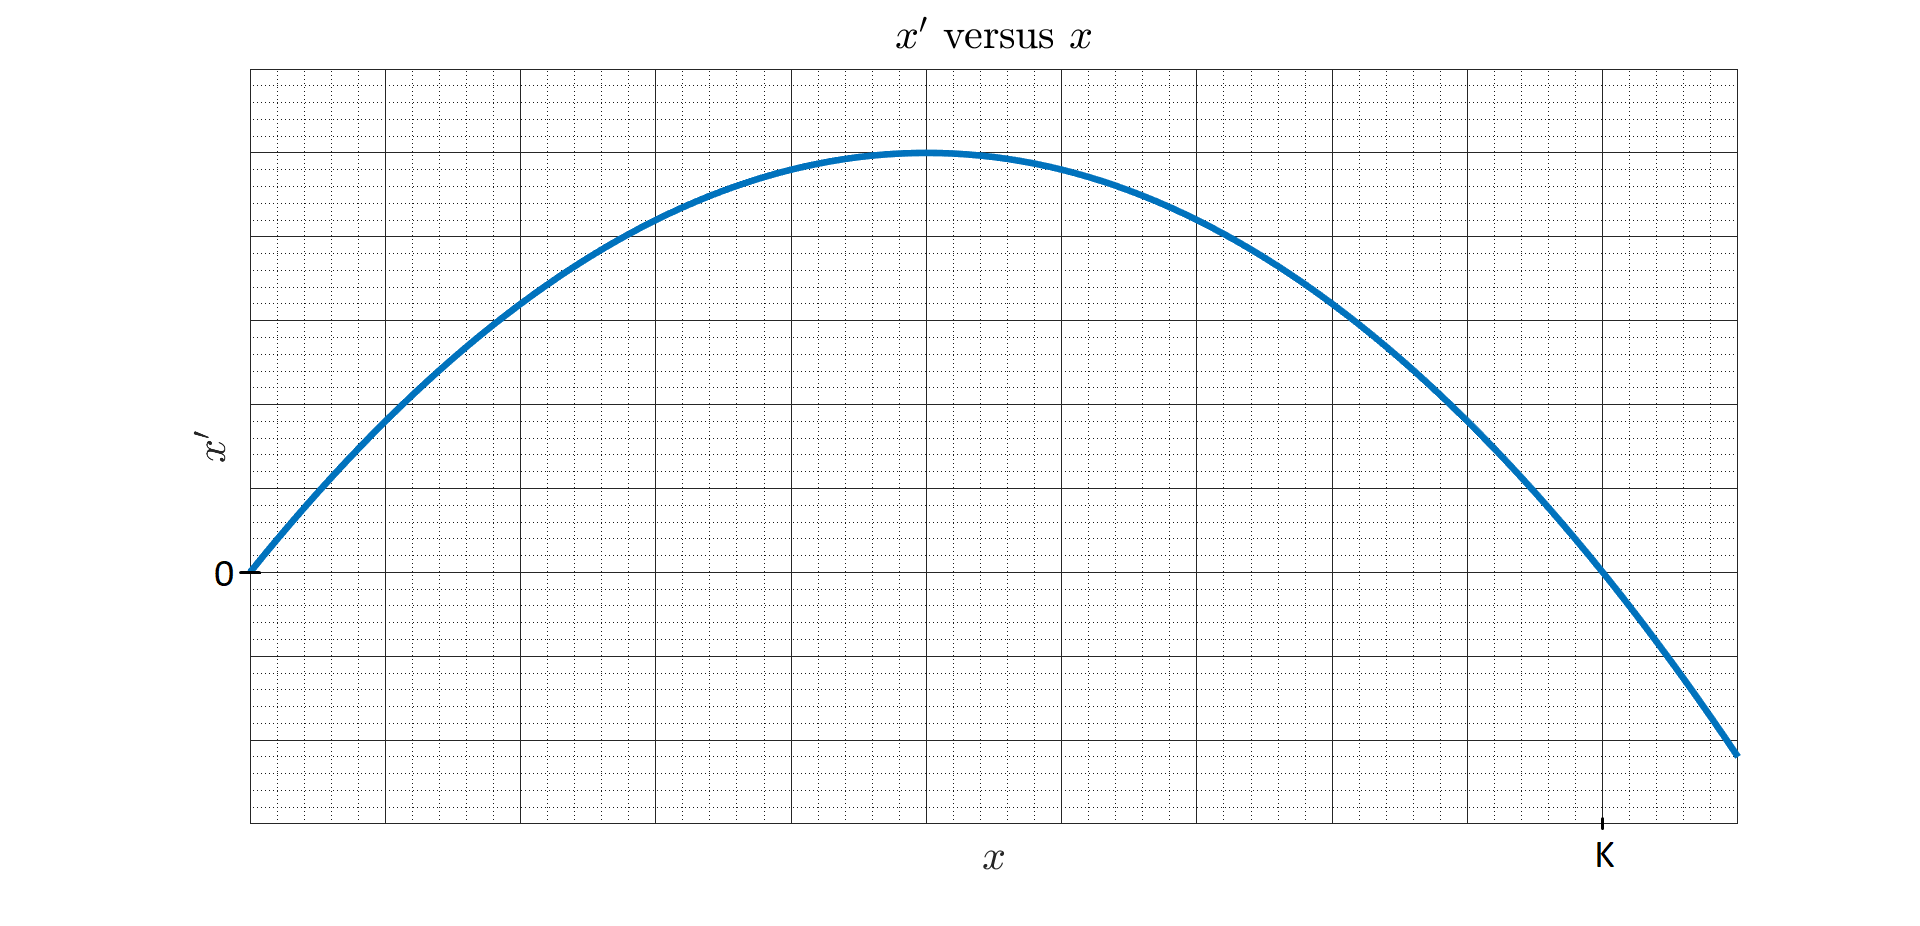
\includegraphics[width=14cm]{Pictures/ODE/LogODE.png}
%     \caption{Plot of the logistic growth equation as a function of $x$.}
%     \label{fig:logisticgrowthODE}
% \end{figure}
% The figure above illustrates that the population, $x$, will continue to grow when $x<K$, but decrease when $x>K$. The population will always be converging towards $K$, which is what we would expect to see in the real world. Thus, the logistic model is a more accurate representation of a specie's population.

% % by using the Lotka-Volterra equation an interaction between two species can be modeled.

\section{Logistic Model For Pacific Salmon}

The Alaskan rivers and streams are comprised of 5 species of salmon; sockeye \emph{O. nerka}, chinook \emph{O. tshawytscha}, coho \emph{O. kisutch}, chum \emph{O. keta}, and pink \emph{O. gorbuscha}.
Of the 5 species, sockeye salmon is the most common food source for Alaskan brown bears~\cite{ADFGsalmon}.
Sockeye salmon begin their journey hatching in streams and making their way down to the ocean.
At this point, they spend a year to 2 years out at sea before migrating back to the streams where they originated.
According to the National Park Service (NPS), only $25-40\%$ of returning salmon in Bristol Bay, Alaska, escape harvesting from commercial fisheries~\cite{NPS}.
They will then travel several miles upstream, where they lay and fertilize their eggs, called spawning.
Salmon will then lay between 1,500 to 10,000 eggs when spawning, but only 0 to 10 of these eggs will reach adulthood~\cite{WFRC}.
A significant proportion of energy for spawning salmon is spent reaching an optimal place to lay and fertilize their eggs, so much so that once they finish this process, they usually die shortly after~\cite{ADFGsalmon}. 

Based on the information above, the rate at which the salmon population grows appears to be exponential.
On average, for every salmon that lays eggs, 5 of their offspring will survive long enough to be adults ready to migrate back to their birthplace. Then, according to the NPS, approximately 32\% of those 5 offspring will make it past escapement to reproduce. These conditions allow us to model the salmon population, shown below,
\begin{equation}\label{eq:fishexpbase5}
    x(t) = x_0(0.32*5)^t,
\end{equation}
where $x_0$ is the initial number of salmon that laid eggs and $t$ represents time in years. We can then rewrite this exponential function with base $e$, as shown below,
\begin{equation}\label{eq:fishexp}
    x(t) = x_0e^{r_xt},
\end{equation}
where $r_x=\ln{(0.32*5)}$ represents the growth rate. Taking the derivative of $x(t)$ give us the salmon population's instantaneous rate of change,
\begin{equation}\label{eq:fishexpdif}
    \frac{dx}{dt} = r_xx_0e^{r_xt} = r_xx.
\end{equation}
% The above first order ordinary differential equation is now represented as the exponential growth model discussed in chapter 2. 
To examine the solution of the above model, we plot the function with an initial starting point of $20$.
% \begin{figure}[H]
%     \centering
%     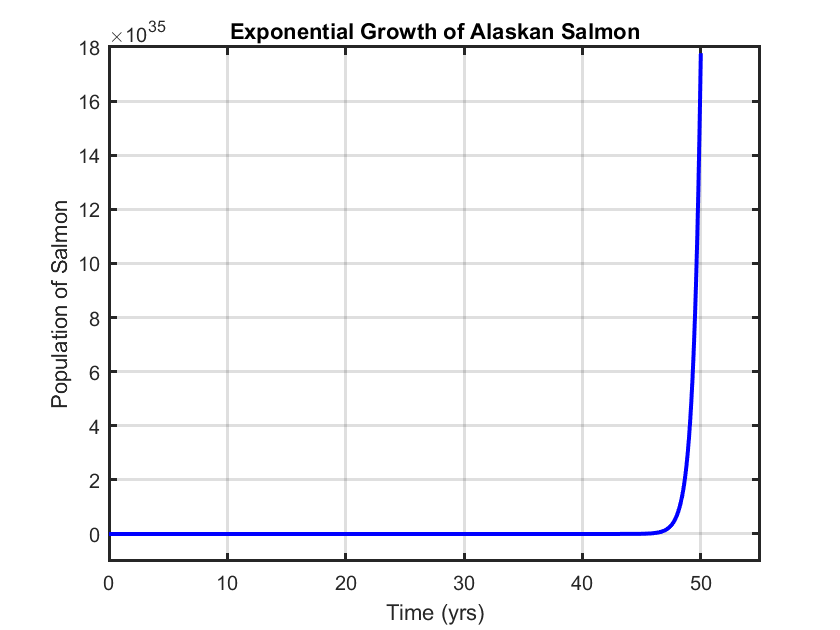
\includegraphics[width=14cm]{Pictures/Salmon Pop/Fish Exponential.png}
%     \caption{The plot above illustrates the population of salmon increasing exponentially resulting in a total of approximately \num{1.8e36} salmon after 50 years.}
%     \label{fig:salmonexp}
% \end{figure}
% Judging from the figure above the population appears quite small until around year 47.
% The population at the 47 year mark is approximately \num{5.7e32} salmon which is not small at all.
% To see this trend a little bit better the graph below is the same plot but for 2 years instead of 50.
\begin{figure}[H]
    \centering
    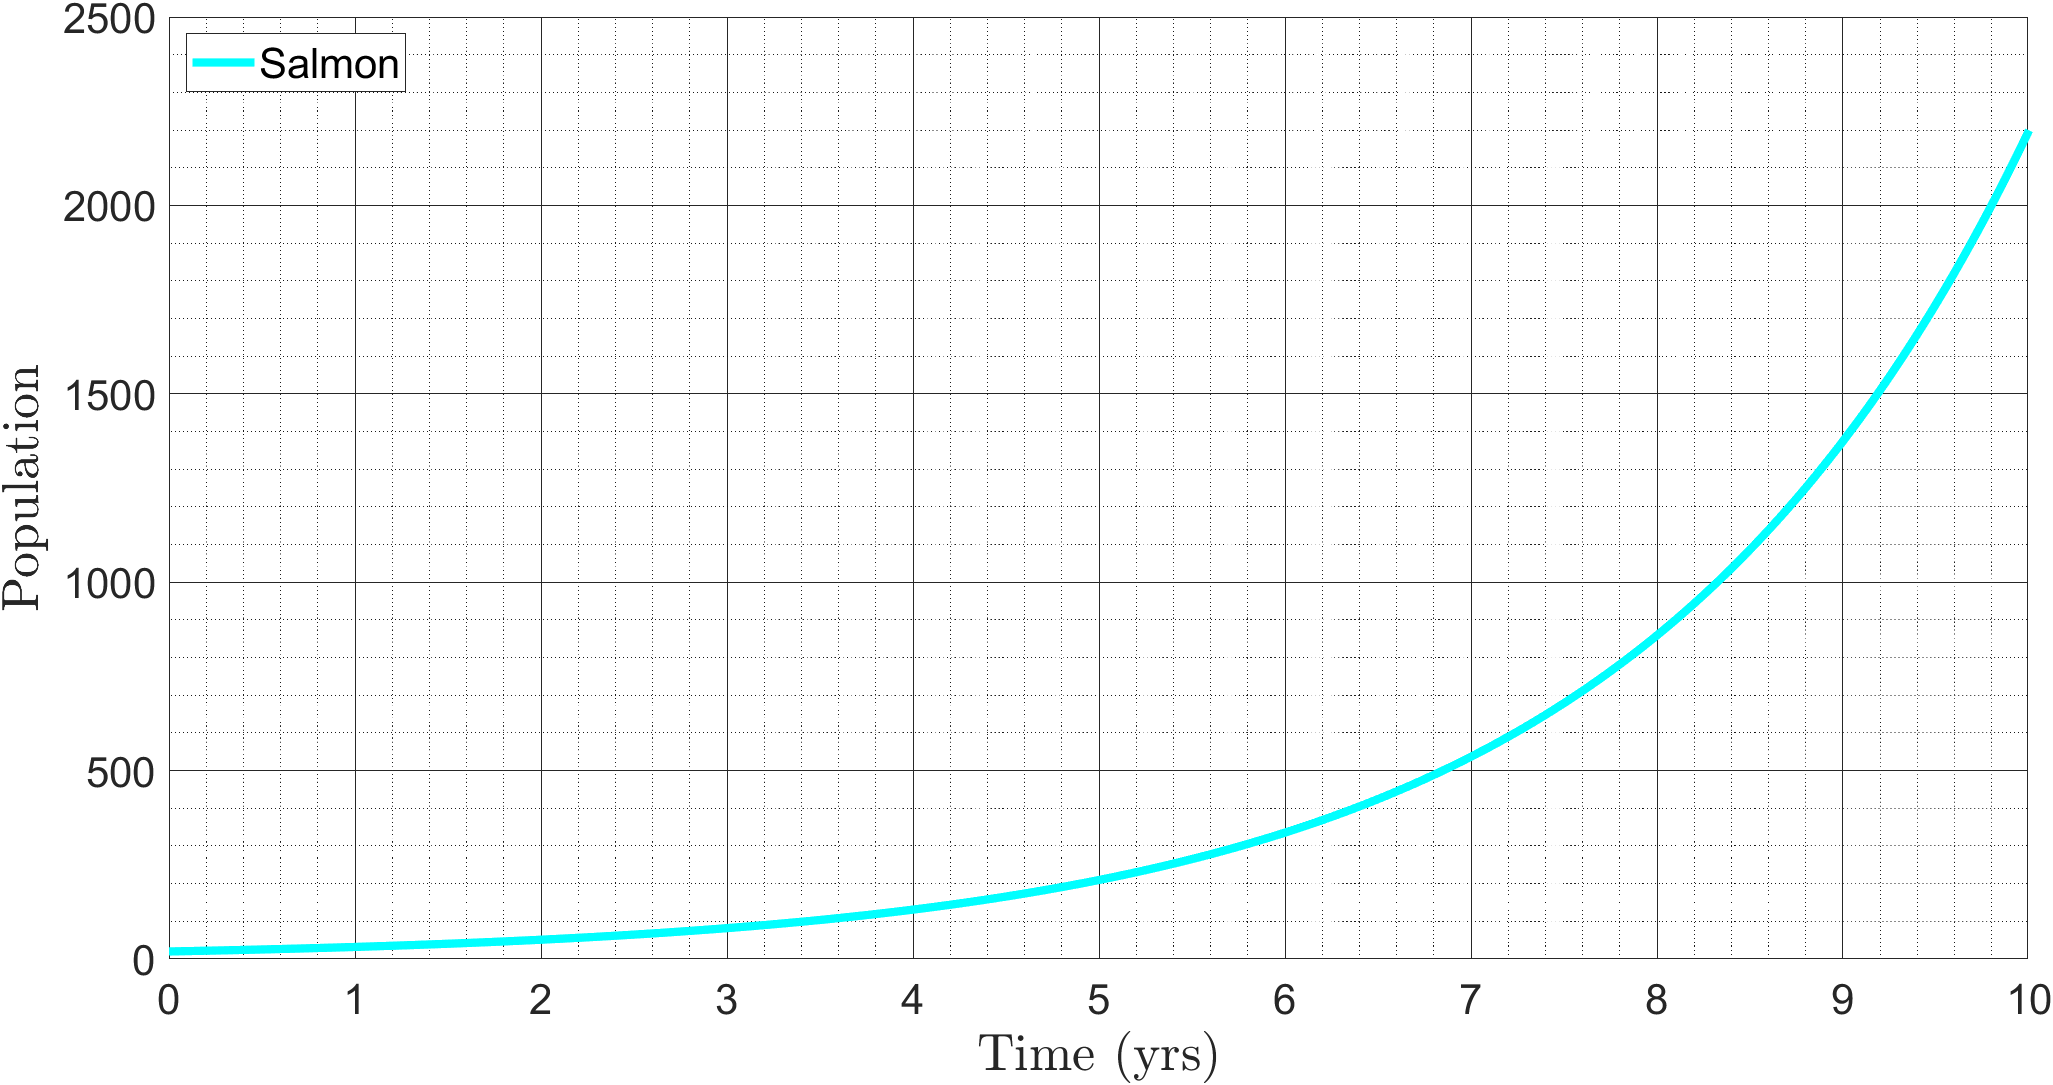
\includegraphics[width=14cm]{Pictures/Salmon Pop/SalmonExpo.png}
    \caption{\singlespacing
    Plot of the exponential growth model for the salmon population with respect to time.}
    \label{fig:salmonexpzoom}
\end{figure}
This figure illustrates that the population of salmon increases quickly in a short period.
In just 9 years, the population of salmon increases from 20 to approximately 1,400, and 1 year later, the population grows to about 2,200. 
The issue with this model is that the population gets extremely large in a short period of time, eventually reaching values that would fall well outside physical possibility.
Now that we have established a growth rate, a carrying capacity can be estimated using data from the ADFG in Bristol Bay, Alaska.

Bristol Bay is located on the easternmost side of the Bering Sea and is where many salmon migrate when returning home to reproduce.
There was a dramatic increase in sockeye salmon returning to Bristol Bay in 2021 compared to previous years. However the average weight of sockeye salmon this year decreased by a pound compared to the average for the past 20 years~\cite{bristol}.
% In Bristol Bay, there are 5 different species of salmon: sockeye \emph{O. nerka}, chinook \emph{O. tshawytscha}, coho \emph{O. kisutch}, chum \emph{O. keta}, pink \emph{O. gorbuscha} \cite{bristol}.
The sockeye species make up a large majority of the inshore runs, harvests\footnote{Harvests is defined as the number of fish gathered by commercial fisheries.}, and escapements\footnote{Escapements are salmon that escape the fisheries and continue upstream to spawn.} in Bristol Bay each year, which explains why the brown bear population mainly feeds on sockeye salmon~\cite{bristol}.
\begin{table}[H]
\rowcolors{2}{white!40}{lightgray!40}
    \centering
    \caption{Sockeye Comparison Between Weight and Run Size in Bristol Bay}\label{tab:weightvsrunshort}
    \vspace{.25cm}
    \begin{tabular}{|c|c|c|}
    \hline
         \textbf{Year} & \textbf{Weight (lbs)} & \textbf{Run (mil)} \\
    \hline
         2001 & 6.7 & 22.3\\
         2002 & 6.1 & 16.9\\
         2003 & 6.3 & 24.9\\
         2004 & 5.8 & 41.9\\
         \vdots & \vdots & \vdots\\
         2017 & 5.5 & 57.6\\
         2018 & 5.1 & 63.0\\
         2019 & 5.1 & 56.4\\
         2020 & 5.1 & 58.3\\
         2021 & 4.7 & 67.7\\
         \hline
    \end{tabular}
    \vspace{1ex}
    
    {\singlespacing
    % \raggedright 
    *This table gives a brief look at the relationship between run size and the average annual weight of sockeye salmon in Bristol Bay. 
    See \tablename~\ref{tab:runvsweight} in \appendixname~\ref{appendix:salmon} for the complete data.\par}
\end{table}
In the first 3 years of this table, the weight seems to be dramatically higher than in the last 3 years, but the opposite effect appears in run size.
This proposes the question that there might be a correlation between the run size and the average weight of salmon each year.
When taking a closer look at \tablename~\ref{tab:runvsweight} in \appendixname~\ref{appendix:salmon}, the trend becomes more apparent when comparing the sockeye's run size and the average annual weight.
Before calculating the correlation between these two events, we must create a plot to see if the trend is linear.
\begin{figure}[H]
    \centering
    \includegraphics[width=14cm]{Pictures/runVSweight/runVSweightNoTitle.png}
    \caption{\singlespacing
    Scatter plot of the variables; inshore run size and the average weight of salmon during that year's run, with the line of best fit.}
    \label{fig:runvsweight}
\end{figure}
Based on the figure above, there is a linear correlation between sockeye run size and their average weight.
The run size of the sockeye salmon decreases as their average weight increases. 
Since multiple variables make up the size of a salmon run each year, this helps explain the variance seen in the plot.
So, calculating the correlation of these two events gives a value of $-0.88$.
Since the correlation of these events is strong, an environmental limit of salmon can be estimated based on the maximum annual volume of sockeye salmon for the past 21 years.
When looking at \tablename~\ref{tab:volume} in \appendixname~\ref{appendix:salmon}, the maximum volume for any given run in the last 21 years was $7.34$ million cubic feet (MMCF) in $2018$. 
The average weight of sockeye salmon during this year was $5.1$ lbs, which is $0.4$ lbs more than the lowest average weight of $4.7$ lbs in 2021.
Now, the carrying capacity for sockeye salmon can be estimated using the maximum volume and the lowest average weight, producing a value of $68.4$ million sockeye salmon.
Sockeye are not the only salmon in the river streams, but according to 
\tablename~\ref{tab:harvestBristol} in \appendixname~\ref{appendix:salmon}, they make up approximately $94\%$ of the average annual commercial harvest in Bristol Bay.
Assuming that the run proportions are the same as the average annual commercial harvest, $72.8$ million becomes the carrying capacity for inshore salmon runs in Bristol Bay.
As stated earlier, approximately 32\% of adult salmon will escape commercial harvesting, which changes the carrying capacity to $29.1$ million salmon each year~\cite{NPS}.


Now that we have the carrying capacity of the salmon population, we can construct their logistic growth model to be
\begin{equation}\label{eq:fishlogistic}
    \frac{dx}{dt} = r_xx\left(1-\frac{x}{K_x}\right),
\end{equation}
where $K_x=29,100,000$ is the carrying capacity, and $r_x=\ln{(0.32*5)}$ is the growth rate.
If we start with an initial population of $20$ million, the population should have the below trend.
\begin{figure}[H]
    \centering
    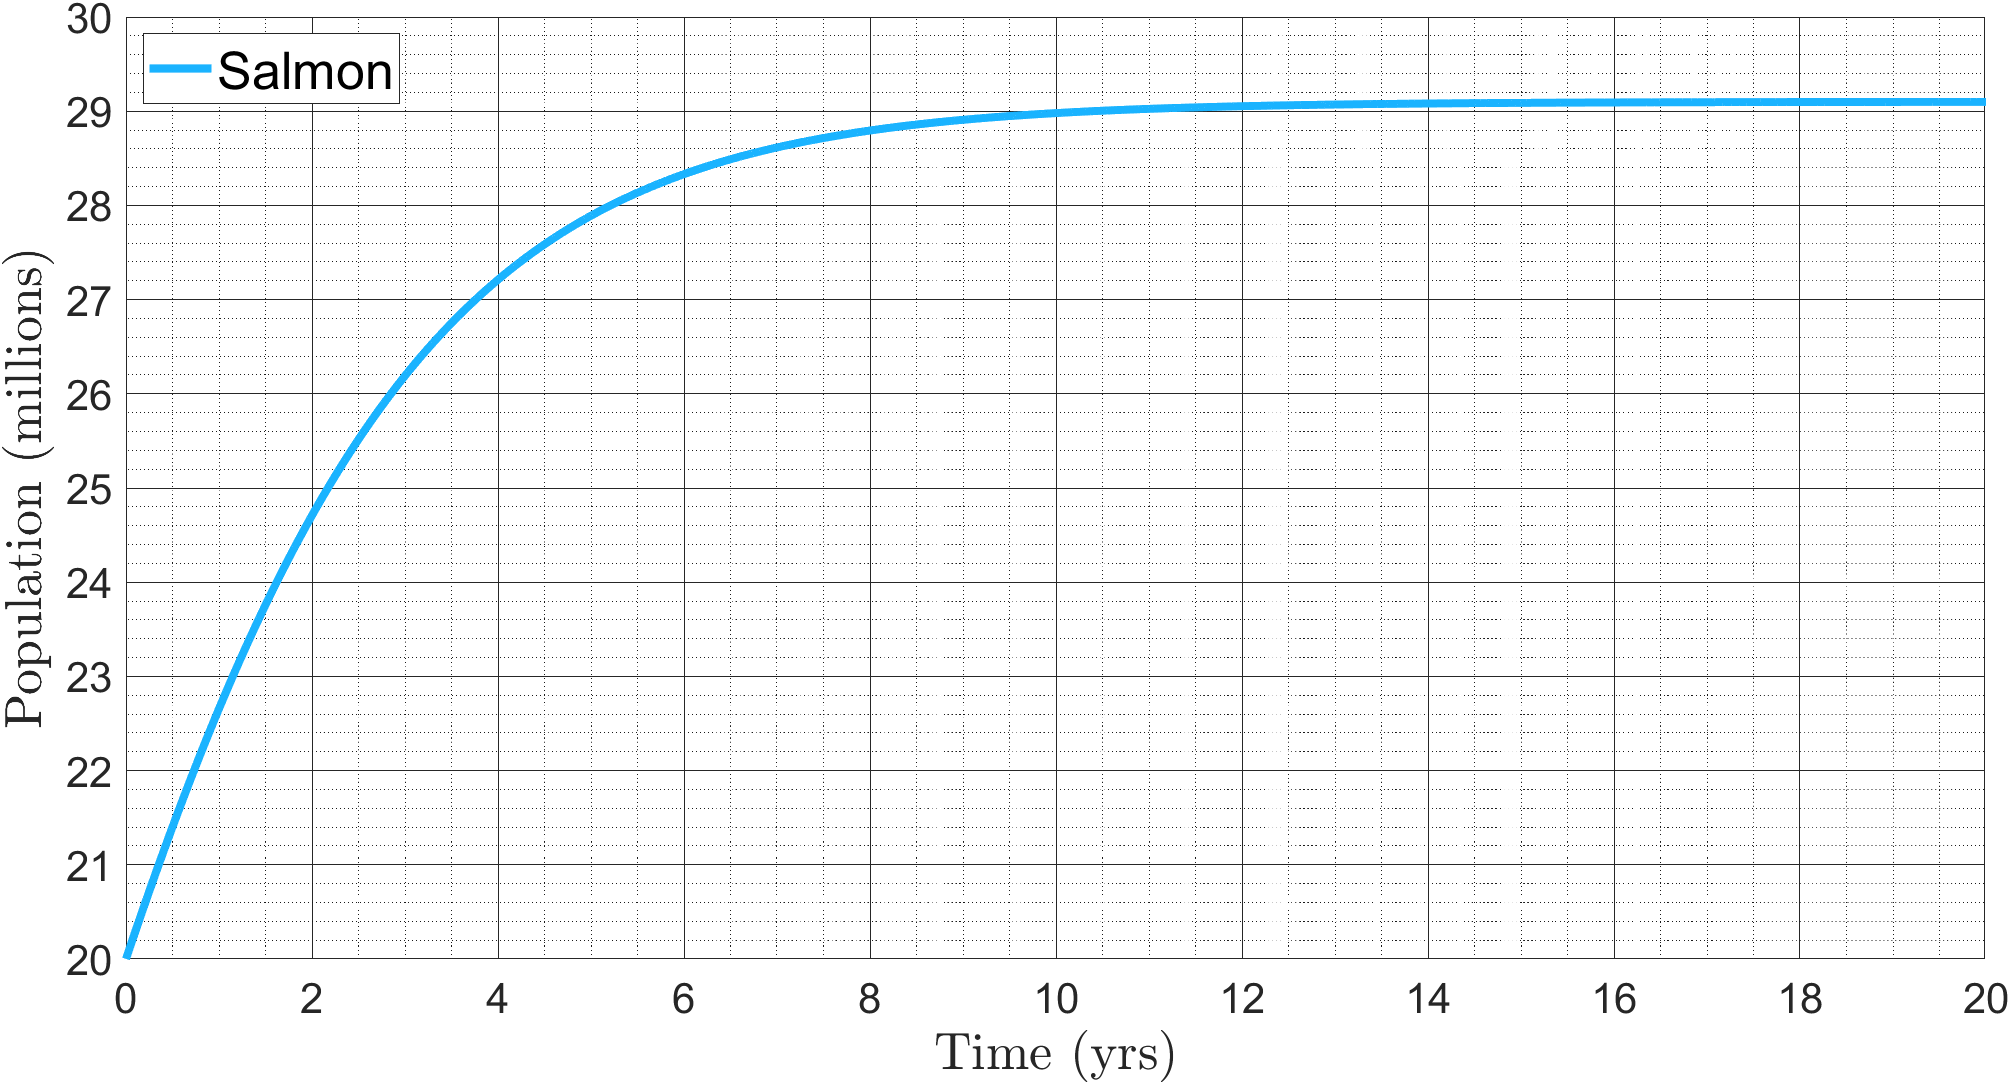
\includegraphics[width=14cm]{Pictures/Salmon Pop/SalmonLogistic.png}
    \caption{\singlespacing
    Plot of the logistic growth model for the salmon population with an initial population of $20$ million.}
    \label{fig:salmnologistic}
\end{figure}
From the graph above, the population of salmon grows rapidly for about 14 years before approximately reaching the carrying capacity.
In the next chapter, we will examine if the changes in temperature affect the growth rate of salmon, and if so, incorporate climate change into the model and evaluate the results.



% Cooper Creek, Kenai River, Russell Creek, Terror River, and Staney Creek





% \begin{itemize}
%     \item Pacific coast salmon lay between 1500 to 10000 eggs.
%     \item 0 to 10 survive to adult hood
%     \item According to the Alaskan government the population of sockeye Salmon follow a logistic curve for each year.
%     \item They grow exponentially but there is a carrying capacity.
% \end{itemize}

\section{Logistic Model For Alaskan Brown Bears}

Throughout this thesis, the logistic model for the Alaskan brown bear population will be of the form,
\begin{equation}\label{eq:LogBear}
    \frac{dy}{dt} = r_yy\left(1-\frac{y}{K_y}\right).
\end{equation}
Researchers Lawrence J. Van Daele and Victor G. Barnes Jr. wrote a report ``MANAGEMENT OF BROWN BEAR HUNTING ON KODIAK ISLAND, A\-L\-A\-S\-K\-A'' in 2010 that discusses the growth of the brown bear population and harvest strategies to maintain a healthy species~\cite{daele2010management}.
They collected data using aerial surveys in Kodiak Archipelago and developed a deterministic population model using RISKMAN, a RISK MANagement Decision Tool~\cite{daele2010management,deterministic}. From the model, they approximated a growth rate of $\lambda=1.014$ for Kodiak bears.
So, we estimate $r_y=\ln(1.014)\approx0.014$ to be the stochastic growth rate for Barnes' and Van Daele's deterministic model.
% According to Barnes' and Van Deale's analysis of their deterministic population model, the growth rate of the Alaskan brown bear population should be $r_y = 0.014$~\cite{daele2010management}.

% Now, according to the Alaska Fish \& Game Department (ADFG), the current recorded population for brown bears is estimated to be 30,000 \cite{ADFG}.
% The population shouldn't reach more than 40,000 to 50,000 due to environmental control, so it seems fair to keep the carry capacity around there \cite{ADFG}. 
% 
% From the data collected by \cite{wielgus1994dynamics,daele2010management} a graph below is produced.
% \begin{figure}[H]
%     \centering
%     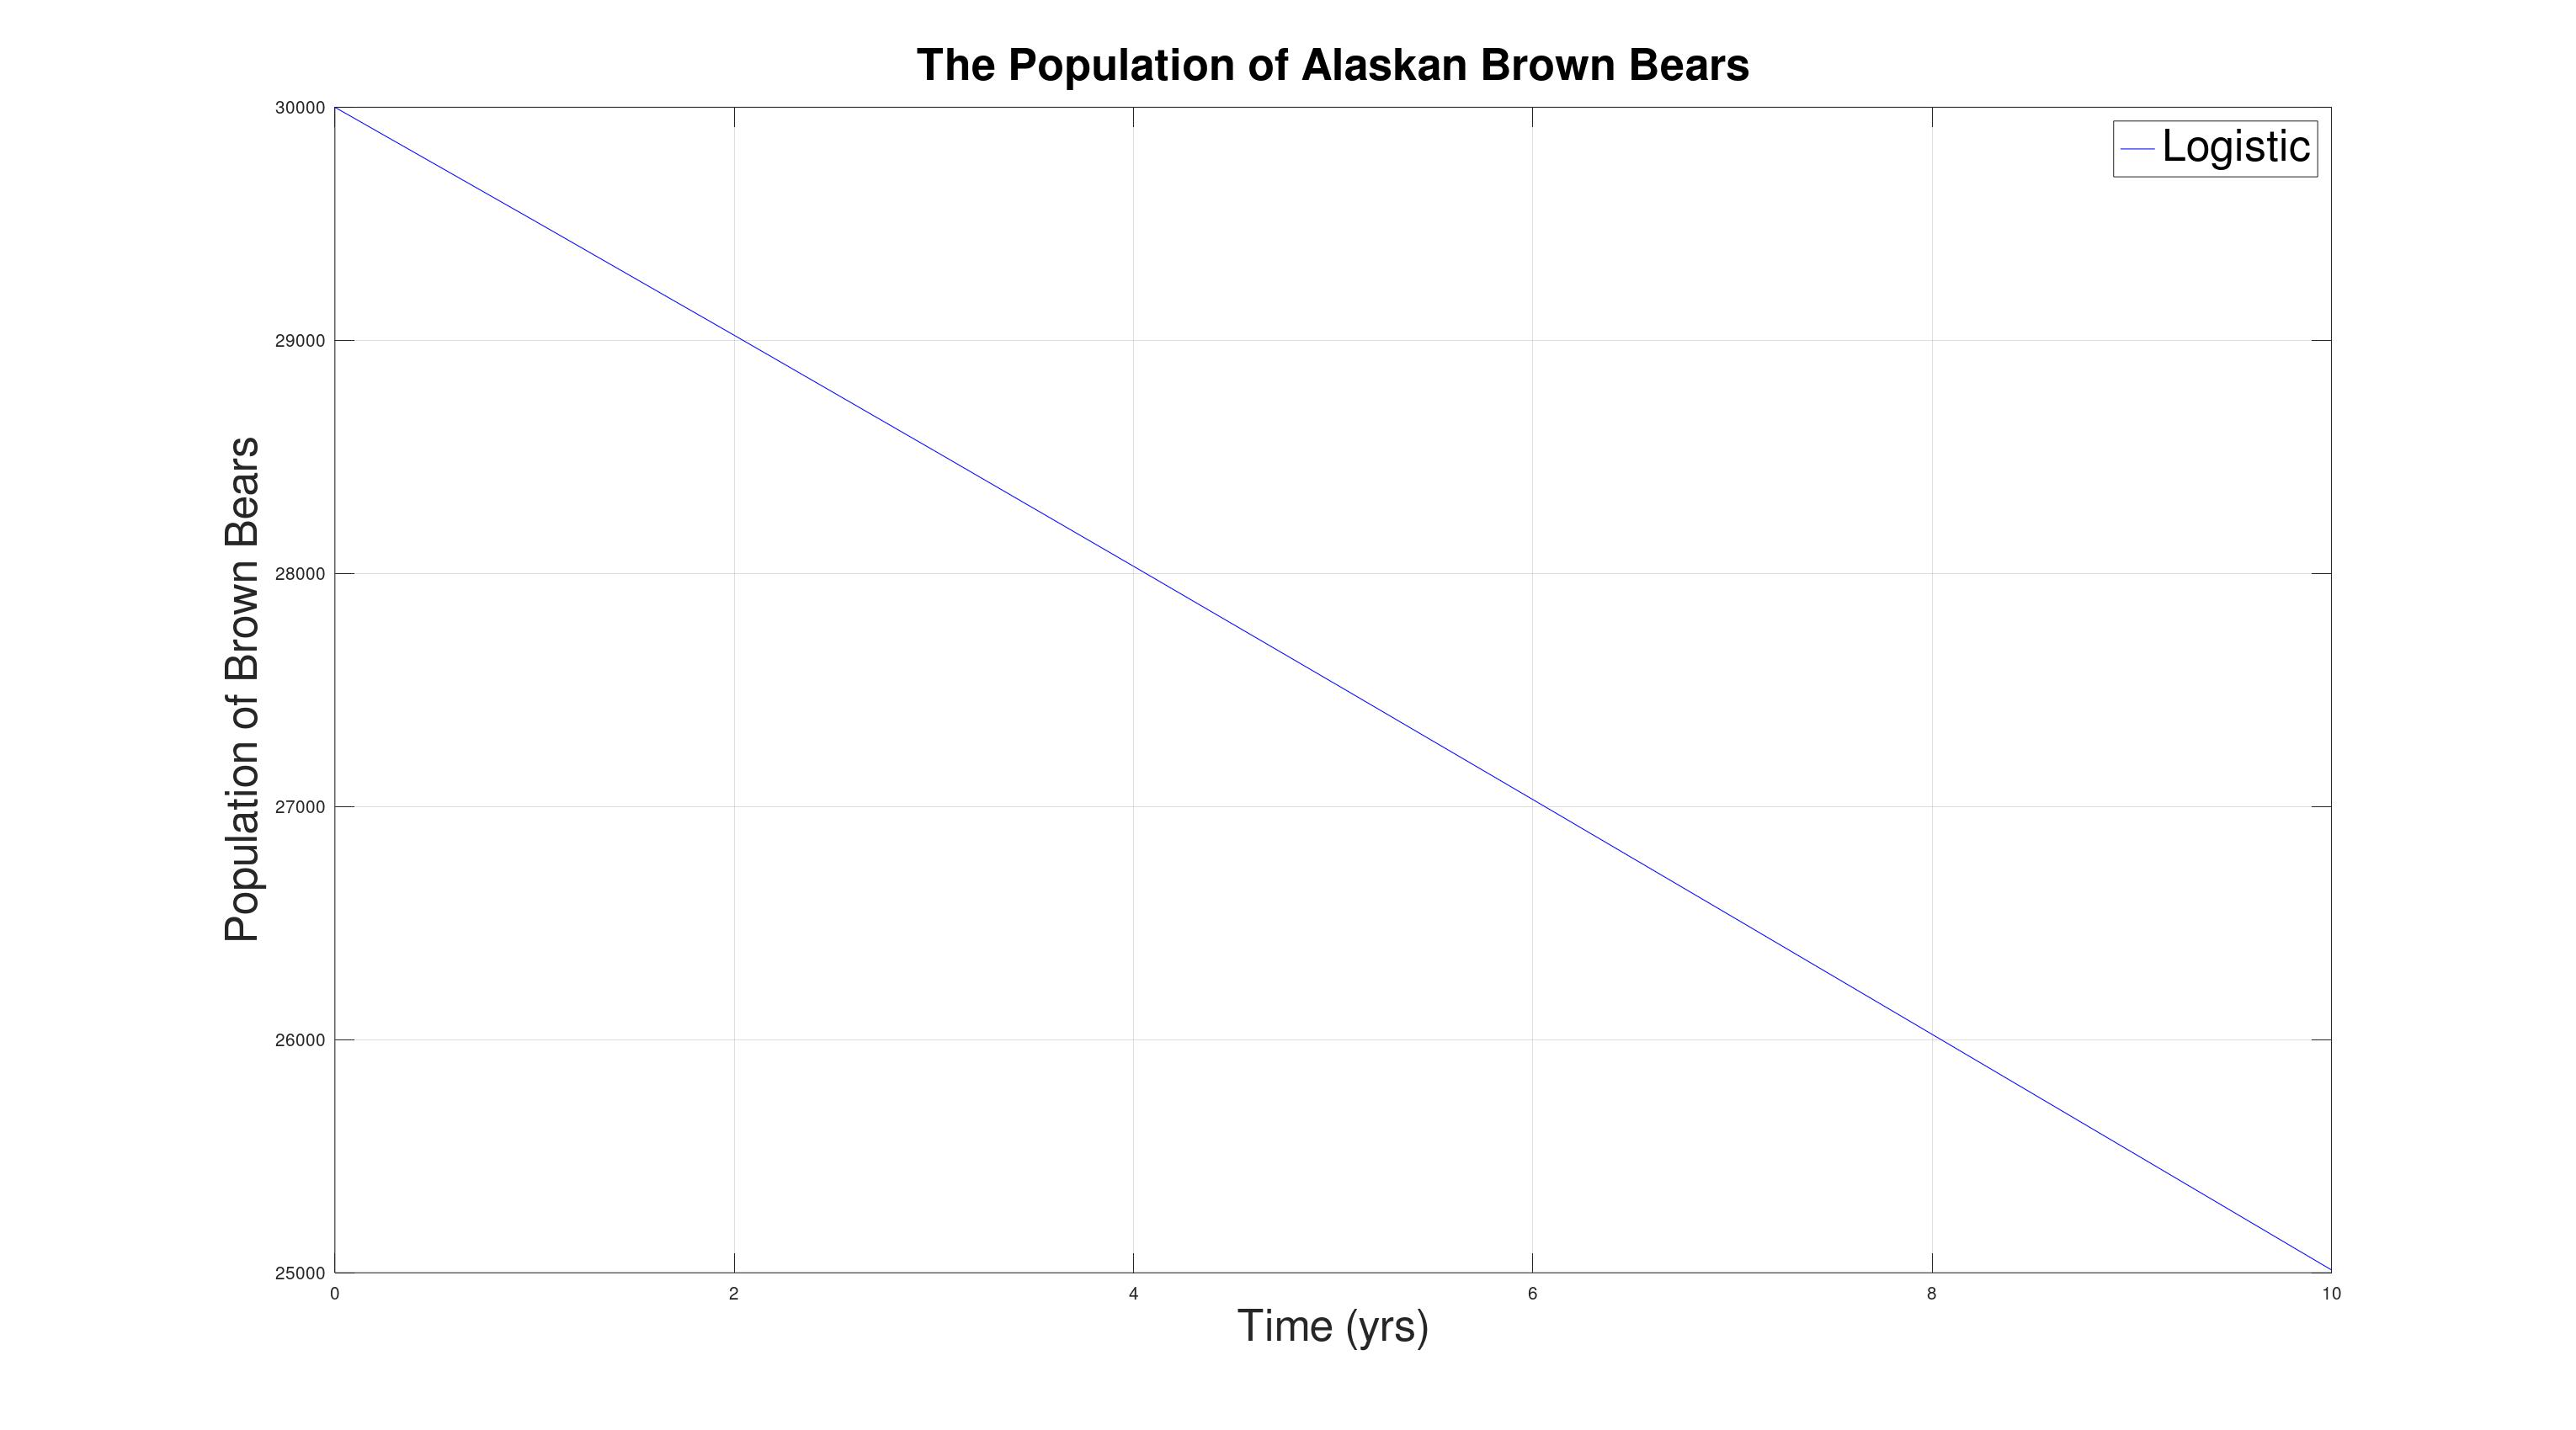
\includegraphics[width=14cm, height=8cm]{Pictures/Population_daele.jpg}
%     \caption{Using the combined data from the Van Daele's and Wielgus' articles, we can plot a prediction of the Alaskan brown bear population after 10 years\cite{daele2010management,wielgus1994dynamics}. The population decreases by 16.63\% over those 10 years.}
%     \label{fig:PopVD}
% \end{figure}
% From this graph we can see that the population is definitely decreasing over time. The end predicted population after 10 years is 25,012 which implies a 16.63\% decrease in population over that time frame. While \cite{daele2010management} seemed to have predicted an increase in population, the construction of their model isn't available to compare against. Van Daele and Barnes did compare their result to other article and found similar results produce by the basic logistic growth model, \equationautorefname~\eqref{eq:basicgrowth} \cite{daele2010management}. From Van Daele and Barnes discussion models ranged from about 16.6\% increase over 10 years and a 19\% decrease over 11 years\cite{daele2010management}. A reason for the difference in population growth could be the area the data was collected in.
% \\

% An article that is similar to Barnes' and Van Daele's management report was produced by Robert B. Wielgus and Fred L. Bunnell that investigated the growth rate of brown bears in Kananaskis Park and Bow Crow Forest of 
% southwestern Alberta, Canada~\cite{wielgus1994dynamics}.
% Wielgus and Bunnell collected their data by trapping and placing collars on their sample.
% Once the survival and reproduction rate was estimated from the data, they implemented the Lotka-Volterra equation to approximate their growth rate $r_y = \pm 0.01$.

Van Daele and Barnes compare their results to Bruce N. McLellan's research on the dynamics of grizzly bears.
McLellan's article, ``Dynamics of a grizzly bear population during a period of industrial resource extraction. III. Natality and rate of increase,'' used the Lotka equation to estimate the growth rate of a grizzly bear population in Flathead Valley, British Columbia from 1979 to 1989~\cite{mclellan1989}.
In this article, McLellan achieves an estimated growth rate of $r_y=0.081$.
In another article, ``Estimating population growth of grizzly bears from the Flathead River drainage using computer simulations of reproduction and survival rates,'' Frederick W. Hovey and Bruce N. McLellan have continued the research, now from 1979 to 1994, in Flathead Valley and chose a different method of estimating the growth rate on the extended data~\cite{mclellan1996}.
Hovey and McLellan used the bootstrap method to improve the accuracy of estimating bias and standard error compared to the method used in McLellan's 1989 article.
With the new method of calculating the growth rate and the increase in data size, Mclellan and Hovey have found similar results to Mclellan's 1989 article, where the newfound growth rate is $r_y=0.082$.

Before comparing these growth rates, a carrying capacity for the brown bear population needs to be estimated.
According to the Alaska Fish \& Game Department (ADFG), the current recorded population of brown bears is estimated to be 30,000 \cite{ADFG}.
From all the articles above, the common consensus is that the ADFG would like to maintain the size of the Alaskan bear population and keep it from climbing much higher than it is currently~\cite{mclellan1989,mclellan1996,daele2010management}.
For this reason, a carrying capacity of $K_y=45,000$ would be an appropriate estimation of the brown bears' environmental size limit.
Now, for comparison, the graphs below display the solutions of \equationautorefname~\eqref{eq:LogBear} for each growth rate.
\begin{figure}[H]
    \centering
    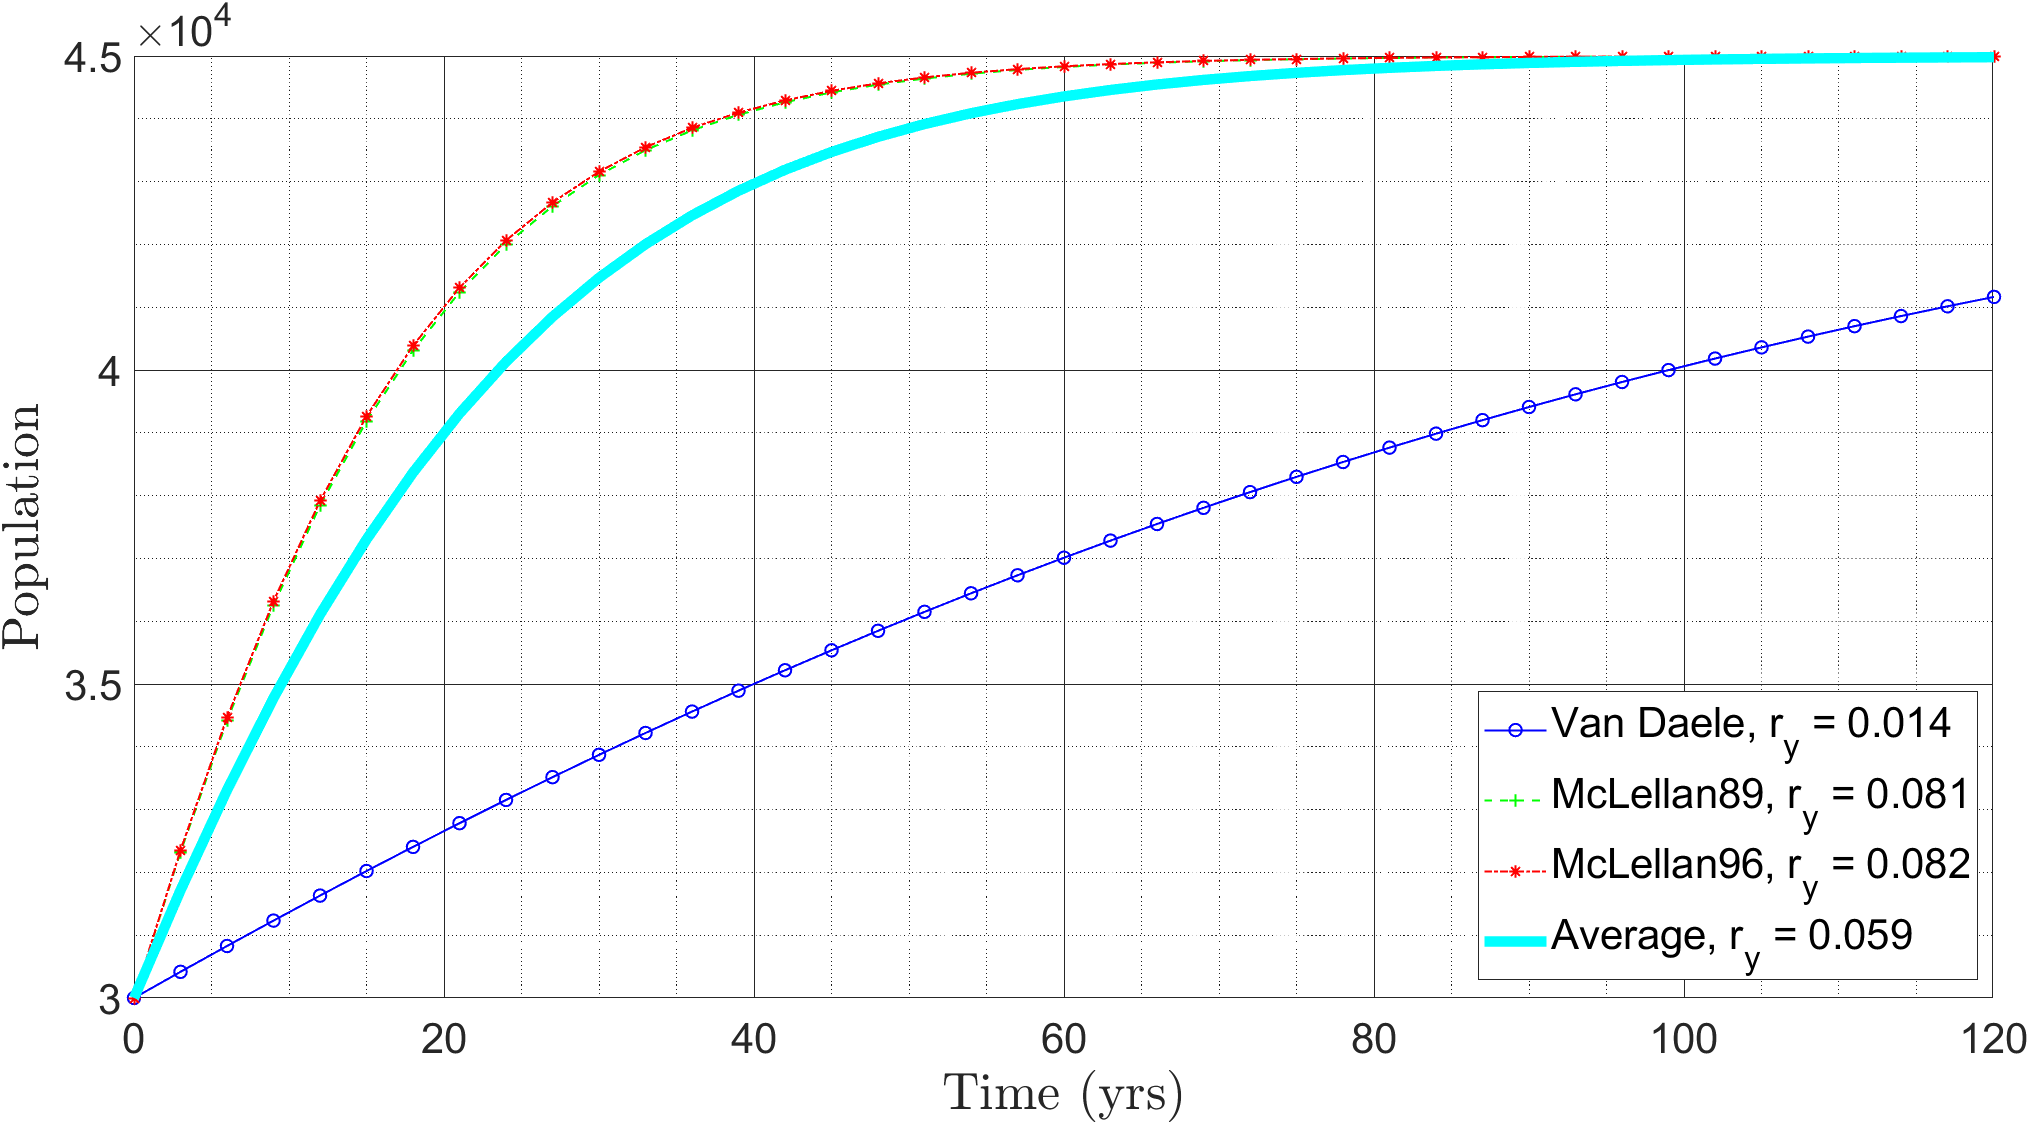
\includegraphics[width=14cm]{Pictures/Bear Pop/different growth rates.png}
\end{figure}
\begin{figure}[H]
    \centering
    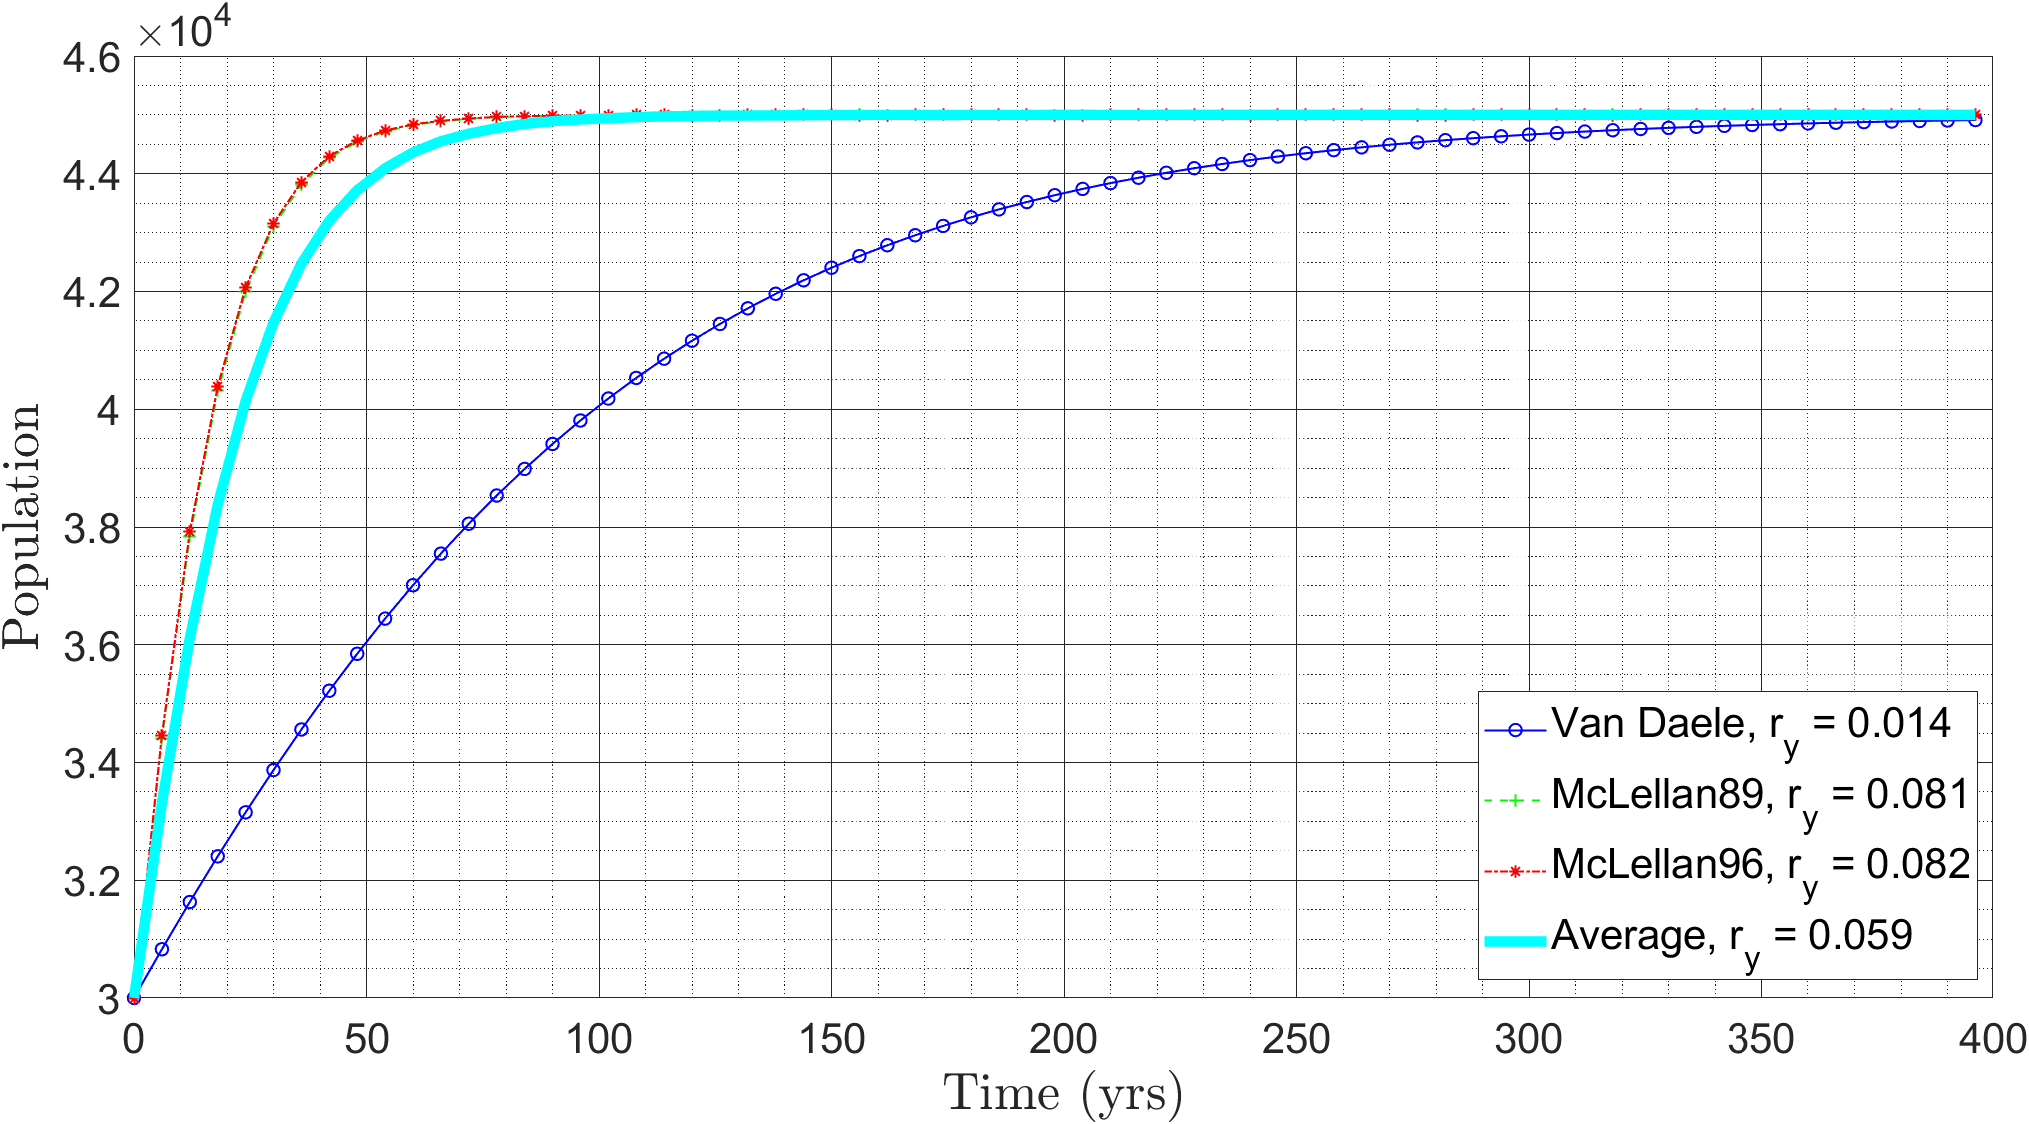
\includegraphics[width=14cm]{Pictures/Bear Pop/different growth rates large.png}
    \caption{\singlespacing
    Plots of the Alaskan brown bear logistic growth equation, \equationautorefname~\eqref{eq:LogBear}, for each of the growth rate parameter values, $r_y$, discussed in the articles above, as well as the average of all the growth rates. 
    The first graph represents a time span of 120 years, and the second represents 400 years.}
    
    % This figure displays the solutions of the logistic growth equation, \equationautorefname~\eqref{eq:LogBear}, for each of the growth rates, $r_y$, from each of the articles discussed above.
    % Also, the mean of all the growth rates is also substituted in the logistic growth model and illustrated with a bold line on the graphs.}
    \label{fig:LogGrowthTrials}
\end{figure}
In the plots above, McLellan's growth rates illustrate that the brown bear population will reach its environmental capacity within 80 years from an initial population of 30,000, while Van Daele's and Barnes' show that it would take the brown bears approximately 400 years.
For this thesis, we estimate the growth rate parameter for the brown bear population by calculating the mean of all the growth rates discussed earlier, resulting in an estimated value of $r_y=0.059$.
\figureautorefname~\ref{fig:LogGrowthTrials} shows that using this growth rate would result in the brown bears reaching their environmental limit in approximately 100 years.

\section{Conclusion}

In this chapter, we proposed a salmon growth rate function that depends on water temperature.
We used river temperature data from the United States Geological Survey (USGS) to design a function that models the increase in Alaskan river temperature over time, which can be seen below,
\begin{equation*}
    T(t) = a*t + b,
\end{equation*}
where $a=0.08$, and $b=9.54$.
Also, $t=0$ represents the current year, 2022.
We then make the growth rate function dependent on time by replacing the temperature parameter $T$ with the temperature function, as shown bellow,
\begin{equation*}
    \begin{array}{ll}
        G(t) &= R(t) + \scalebox{1.2}{$\frac{P'(t)t}{P(t)}$} \\[.2cm]
         &= \ln\left(\scalebox{1.2}{$\frac{0.32*5}{1+10^{-4}(0.08t-2.96)^4}$}\right) - \scalebox{1.2}{$\frac{4*10^{-4}*0.08t(0.08t-2.96)^3}{1+10^{-4}(0.08t-2.96)^4}$}.
    \end{array}
\end{equation*}
Lastly, we replaced this new growth rate function with the growth rate parameter in the original logistic model, \equationautorefname~\eqref{eq:fishlogistic}, and compare its results.
We found that after approximately 100 years, the salmon population will begin to decline and eventually die off or migrate elsewhere.
In the next chapter, we will examine the effect of interaction between the brown bear and salmon species.
We will compare the results of the interaction with and without the growth rate function.

\chapter{Salmon Growth Rate Function}

% Many population growth models use variations of the Verhulst logistic growth equation to simulate the population growth of living organisms.
% James Wallace and Anastasios Tsoularis review different variations of the logistic growth equation in their article, ``Analysis of logistic growth models''~\cite{tsoularis2002analysis}.
% In this thesis, we will use variations of the logistic growth model to describe the populations of pacific salmon and Alaskan brown bears.

In this chapter, we introduce simple logistic growth models for the salmon and brown bear species.
Using information from the Alaskan Department of Fish and Game, we estimate a growth rate parameter for the salmon population.
Then, we choose the carrying capacity parameter by calculating the maximum volume of salmon for any given inshore run\footnote{Inshore runs are when salmon migrate back from the sea to spawn.} in Bristol Bay, Alaska.
We find 3 growth rates from 3 articles for the Alaskan brown bears and calculate their mean, which we use to represent their growth rate parameter~\cite{daele2010management,mclellan1989,mclellan1996}.
Also, for this model, we estimate the carrying capacity based on information from the Alaskan Department of Fish and Game (ADFG)~\cite{ADFG}.



% we begin by creating an appropriate logistic growth model for the brown bear population using growth rates from a few scholarly articles and approximating a carrying capacity from the Alaskan Department of Fish and Game (ADFG). 
% Next, Volhulst’s logistic growth model will illustrate the salmon population using information from the ADFG to achieve a growth rate. 
% Also, the carrying capacity is revealed through the relationship between salmon run size and their average weight during their run. 
% Finally, the chapter briefly compares the two models and introduces the concept of creating a variation of the logistic model that incorporates the aspect of climate change.

\section{Growth Rate Function Dependent on Temperature}

Salmon have an optimal temperature range for the rate at which they grow, migrate, and reproduce. 
If the temperature of their environment goes outside of that range, then salmon may change their spawning location or time frame of migration~\cite{ADFG-optimal}.
If they do not take either of those options, then they may fatigue and die before reaching their spawning location \cite{ADFG-optimal, ADFG-critical}.
So, when temperatures reach a critical point, mortality rates increase significantly, which consequently decreases their growth rate \cite{ADFG-optimal}.
The purpose of this section is to use salmon's mortality rate during spawning migration at different temperatures to approximate a growth rate function, $R(T)$, that is dependent upon temperature.
While there is little research that scientifically describes the effects of salmon population growth at each temperature, there are reports that estimate the optimum temperature range for maximum survival and critical points where survival becomes unlikely.
Dr. Phyllis Weber Scannell wrote an article in 1992 for the Alaskan Department of Fish and Game (ADFG) about the optimal temperature ranges for cold water fish.
In this article, she highlights the optimal range as well as the critical high temperature of sockeye salmon in Alaska~\cite{ADFG-optimal}.
Also, Katherine Carter has published an article that suggests temperatures below $2^{\circ}$C will result in a high mortality rate~\cite{carter2005effects}.\\
% Also, Katherine Carter published an article that we use to suggest that temperatures below $2^{\circ}$C will result in a high mortality rate~\cite{carter2005effects}.\\
\begin{table}[H]
\rowcolors{2}{white!40}{lightgray!40}
    \centering
    \caption{Optimal Temperature Range For Pacific Sockeye Salmon}\label{tab:optimaltemp}
    \vspace{.75cm}
    \begin{tabular}{|c|c|c|c|}
    \hline
         \textbf{Species} & \textbf{Optimal ($^{\circ}$C)} & \textbf{Low ($^{\circ}$C)} & \textbf{High ($^{\circ}$C)}\\
         \hline
         Sockeye & $11-14$ & $<2$ & $>22.2$\\
         \hline
    \end{tabular}
    \vspace{1ex}
    
    {\singlespacing
    % \raggedright 
    *The optimal, critical high and low temperature range for the sockeye salmon species in Alaska \cite{ADFG-optimal, carter2005effects}.\par}
\end{table}
As Dr. Scannel's report states, each researcher estimates slightly different temperature ranges due to a multitude of variables such as acclimation, age, size, genetic strain, and physiological conditions of the fish~\cite{ADFG-optimal}.
That being said, we use \tablename~\ref{tab:optimaltemp} to help fit a curve that best illustrates the impact of temperature on the proportion of salmon that survive their spawning migration.
Now, Katherine Carter's article explains that at these critical points the population could have a mortality rate of 50\%~\cite{carter2005effects}.
% Now, Katherine Carter's article explains that at these critical points the population would have a 50\% mortality rate~\cite{carter2005effects}.
So, we estimate that under ideal conditions and optimal temperatures, 100\% of the salmon population would survive the spawning migration to reproduce, and at critical temperatures, only 50\% would survive.
From \tablename~\ref{tab:optimaltemp} the optimal temperature range is $11-14^{\circ}$C and the critical temperature points are at $2^{\circ}$C and $22.2^{\circ}$C, which can be observed on the graph below.
\begin{figure}[H]
    \centering
    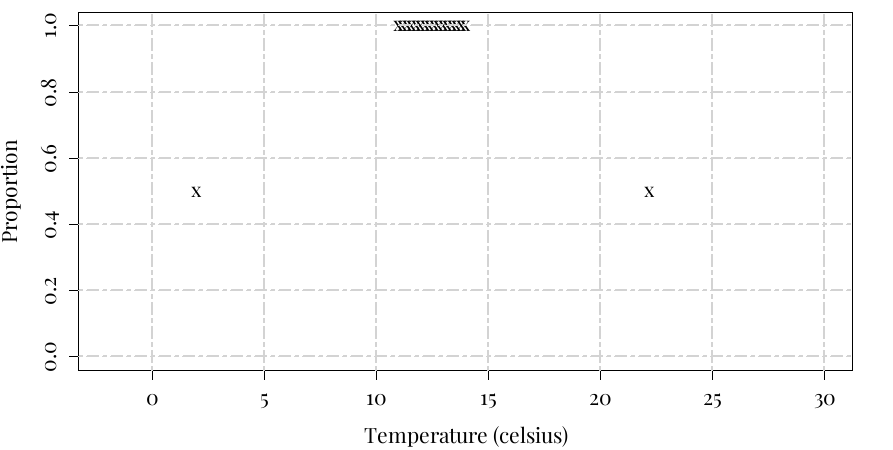
\includegraphics[width=14cm]{Pictures/Salmon Pop/salmon repo model/proportion survival.png}
    \caption{\singlespacing
    Scatter plot of the survival rates in the optimal temperature range and at the critical temperature points.}
    \label{fig:reproductionpoints}
\end{figure}
Given that the width of the optimal range is rather large, developing a function to approximate these data points will be rather difficult.
The proportion of salmon surviving spawning migration cannot drop below 0, which implies that we should be looking at a function similar to the one displayed below,
\begin{equation}\label{eq:repogeneral}
    P(T) = \frac{1}{1+c(T-T_{opt})^p}, \quad p\; \epsilon\; 2\mathbb{N},
\end{equation}
where $P(T)$ estimates the proportion of salmon that will survive spawning migration at a given temperature, $T$, in Celsius, and $T_{opt}$ is the average of the optimal temperature range, $12.5^{\circ}$C. 
The power of the binomial, $p$, controls the average rate of change of the proportions, and $c$ is a constant that will be calculated to stretch or compress the function horizontally.
Now, we get the graph below by setting the parameters $p=2$ and $c=1$ as a starting point for the function above.
\begin{figure}[H]
    \centering
    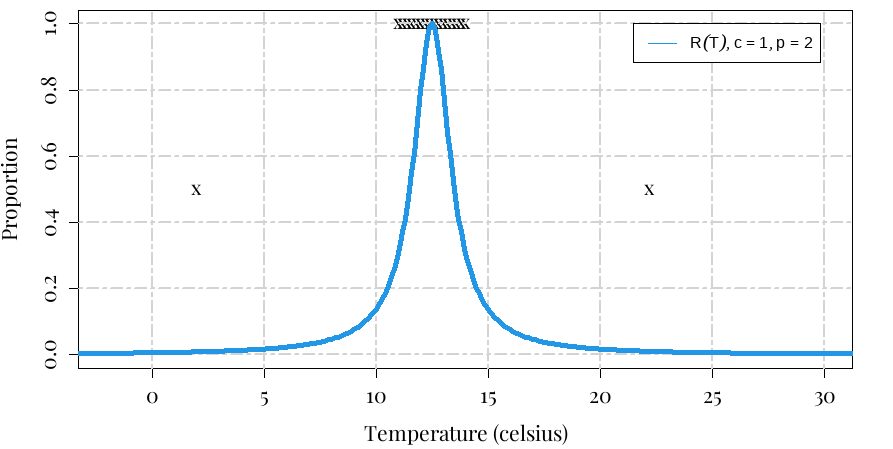
\includegraphics[width=14cm]{Pictures/Salmon Pop/salmon repo model/Repo F2 c1.png}
    \caption{\singlespacing
    Plot of the proportion function, where $c=1$ and $p=2$.}
    \label{fig:reporductioncurve2c1}
\end{figure}
The main issue with these parameters is that the peak of the curve is too narrow to represent the optimal range well, and the curve is too far away from the critical temperature points, $(2,0.5)$ and $(22.2,0.5)$. 
From the graph above, the survival proportion of migrating salmon at the limits of their optimal temperature range is $P(T=11)=P(T=14)\approx0.31$, which is a major deviation from the proposed survival proportion.
So, by adjusting the parameter $c$, we can stretch the function to better fit the survival proportions for the critical and optimal temperatures.
This can be done by taking the average of the distances from $T_{opt}$ to the critical temperatures, as shown below,
\[
Avg = \frac{|T_{opt}-2| + |T_{opt}-22.2|}{2} = 10.1.
\]
From here we can set $P(T)=0.5$ and $T-T_{opt}=Avg=10.1$ and solve for $c$,
\[
c = \frac{1-P(T)}{P(T)(T-T_{opt})^2} = \frac{1-0.5}{0.5(10.1)^2} = \frac{1}{10.1^2} = \frac{1}{102.1}\approx0.01.
\]
Now, plotting $P(T)$ with parameters $p=2$ and $c=0.01$ produces the plot below.
\begin{figure}[H]
    \centering
    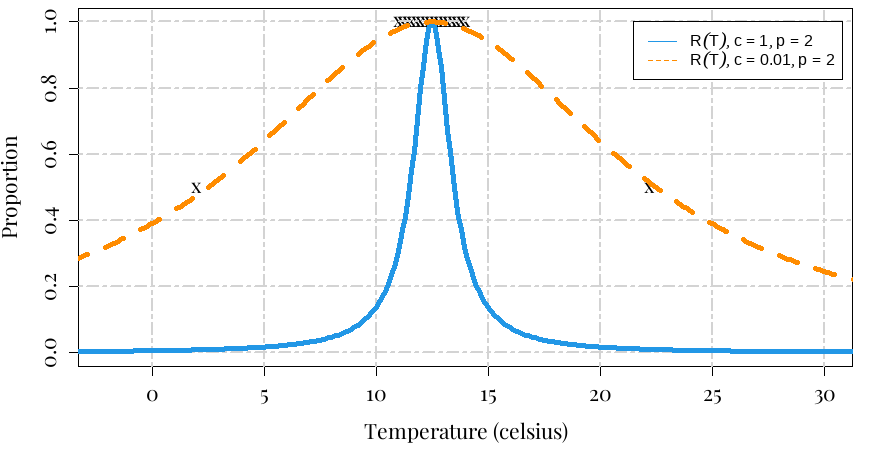
\includegraphics[width=14cm]{Pictures/Salmon Pop/salmon repo model/Repo c1 and c01.png}
    \caption{\singlespacing
    Compares the plots of the proportion function, where $c=1$ and $c=0.01$, but $p=2$ remains the same.}
    \label{fig:reporductioncurve2c1c01}
\end{figure}
From the figure above, the low and high critical temperature points are better represented with the new parameter, $c=0.01$.
However, at the limits of the optimal temperature range, the survival proportion is $0.978$, which should be closer to 1.
This can be resolved by changing the power of the binomial, $p=2$, in \equationautorefname~\eqref{eq:repogeneral} to $p=4$, which will widen the curve while maintaining a steep descent as the temperature escapes the optimal region.
So, substituting the new parameters, $c=0.01$, and $p=4$, the graph below is produced.
\begin{figure}[H]
    \centering
    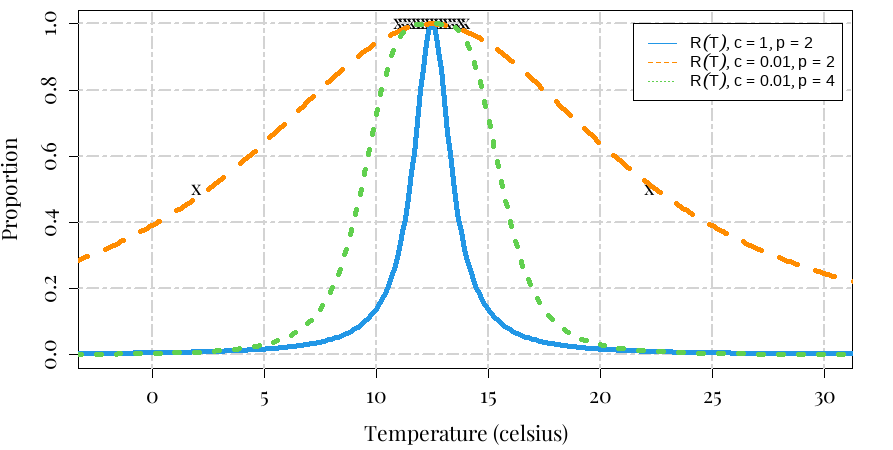
\includegraphics[width=14cm]{Pictures/Salmon Pop/salmon repo model/Repo c1 c01 p4 c01.png}
    \caption{\singlespacing
    Compares the plots of \figureautorefname~\ref{fig:reporductioncurve2c1c01} with the plot of the proportion function, where $c=0.01$ and $p=4$.}
    \label{fig:reproductioncurve2_4_c01}
\end{figure}
With this figure, the representation of the optimal range is better, but the proportions of salmon survival decrease significantly as $T$ approaches the limits of the optimal range.
Also, the survival proportions at the critical temperatures are far from the points, $(2,0.5)$ and $(22.2,0.5)$.
To resolve this issue, we can repeat the same process as earlier to select a new $c$ value that accurately reflects the proportions at the optimal and critical temperatures.
As a result, the graph below is produced by substituting the new parameter $c=10^{-4}$ into the proportion function.
\begin{figure}[H]
    \centering
    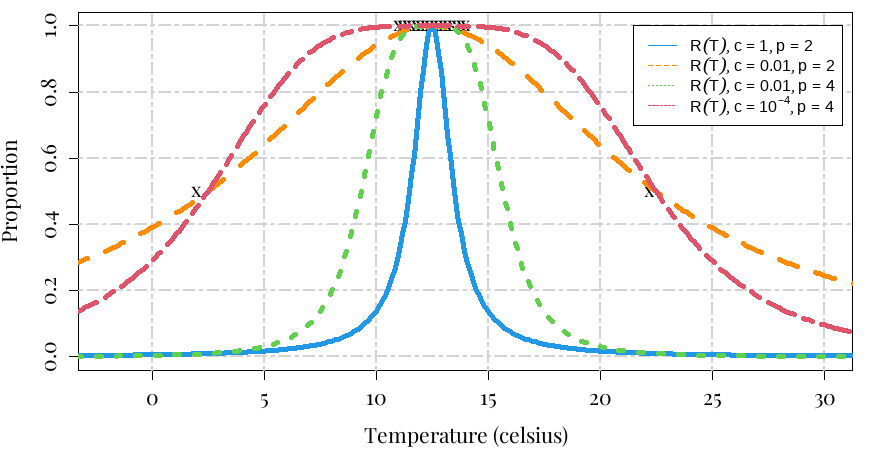
\includegraphics[width=14cm]{Pictures/Salmon Pop/salmon repo model/Repo_all.png}
    \caption{\singlespacing
    Compares the plots of \figureautorefname~\ref{fig:reproductioncurve2_4_c01} with the plot of the proportion function, where $c=10^{-4}$ and $p=4$.}
    \label{fig:reproductioncurve4}
\end{figure}
The parameters, $c=10^{-4}$ and $p=4$, offer a better fit, with the survival proportion being $0.9995$ at the optimal temperature limits and $P(2) \approx 0.45$ and $P(22.2) \approx 0.53$.
By fixing $c=10^{-4},\ p=4$ and $T_{opt}$ in \equationautorefname~\eqref{eq:repogeneral}, we get
\begin{equation}\label{eq:SurvivalProportionFun}
    P(T) = \frac{1}{1+c(T-T_{opt})^p} = \frac{1}{1+10^{-4}(T-12.5)^4},
\end{equation}
where P(T) represents the proportion of salmon that survive spawning migration with respect to temperature.  
During the salmon migration of 2004, Weaver Creek sockeye salmon experienced a drastic rise in water temperature, which resulted in a higher than usual mortality rate~\cite{farrell2008pacific}.
According to Anthony P. Farrell, temperatures were around $20.4^{\circ}$C and 30\% of the salmon population did not make it to the spawning location due to the excessive heat~\cite{farrell2008pacific}.
Using \equationautorefname~\eqref{eq:SurvivalProportionFun}, we get $P(20.4)=0.7197$.
Therefore, we estimate a 72\% survival rate, or a mortality rate of approximately 28\%, for the salmon migrating to their spawning locations, which is close to Anthony P. Farrell's estimation of 30\%.

Looking back, the growth rate, $r_x=\ln{(0.32*5)}$, was estimated when temperatures were ideal, or in the optimal range, so combining the proportion function with the current growth rate, we get the function below,
% \begin{equation}\label{eq:RepoFun}
%     R(T) = 0.32*5*P(T)) = \frac{0.32*5}{1+c(T-T_{opt})^4},
% \end{equation}
\begin{equation}\label{eq:RepoFunLog}
    R(T) = \ln(0.32*5*P(T))  = \ln{\left(\frac{0.32*5}{1+c(T-T_{opt})^4}\right)},
\end{equation}
where $c=10^{-4}$, $T_{opt}=12.5^{\circ}$C, and $T$ is temperature.
% Notice, the proportion function, $P(T)$, is inside the natural log. 
% This is because we want the proportion of salmon that survived the migration after escaping the harvest, which is the same reasoning used when deriving \equationautorefname~\eqref{eq:fishexpbase5}.
Lastly, we will replace the growth rate, $r_x$, with the growth rate function, $R(T)$, in \equationautorefname~\eqref{eq:fishlogistic} to get the below equation,
\begin{equation}\label{eq:salmonlogisticrepo} 
    \frac{dx}{dt} =
    R(T)x\left(1-\frac{x}{K_x}\right).
\end{equation}
To see the effect of temperature on the salmon population, we will compare \equationautorefname~\eqref{eq:salmonlogisticrepo} at different temperatures.
\begin{figure}[H]
    \centering
    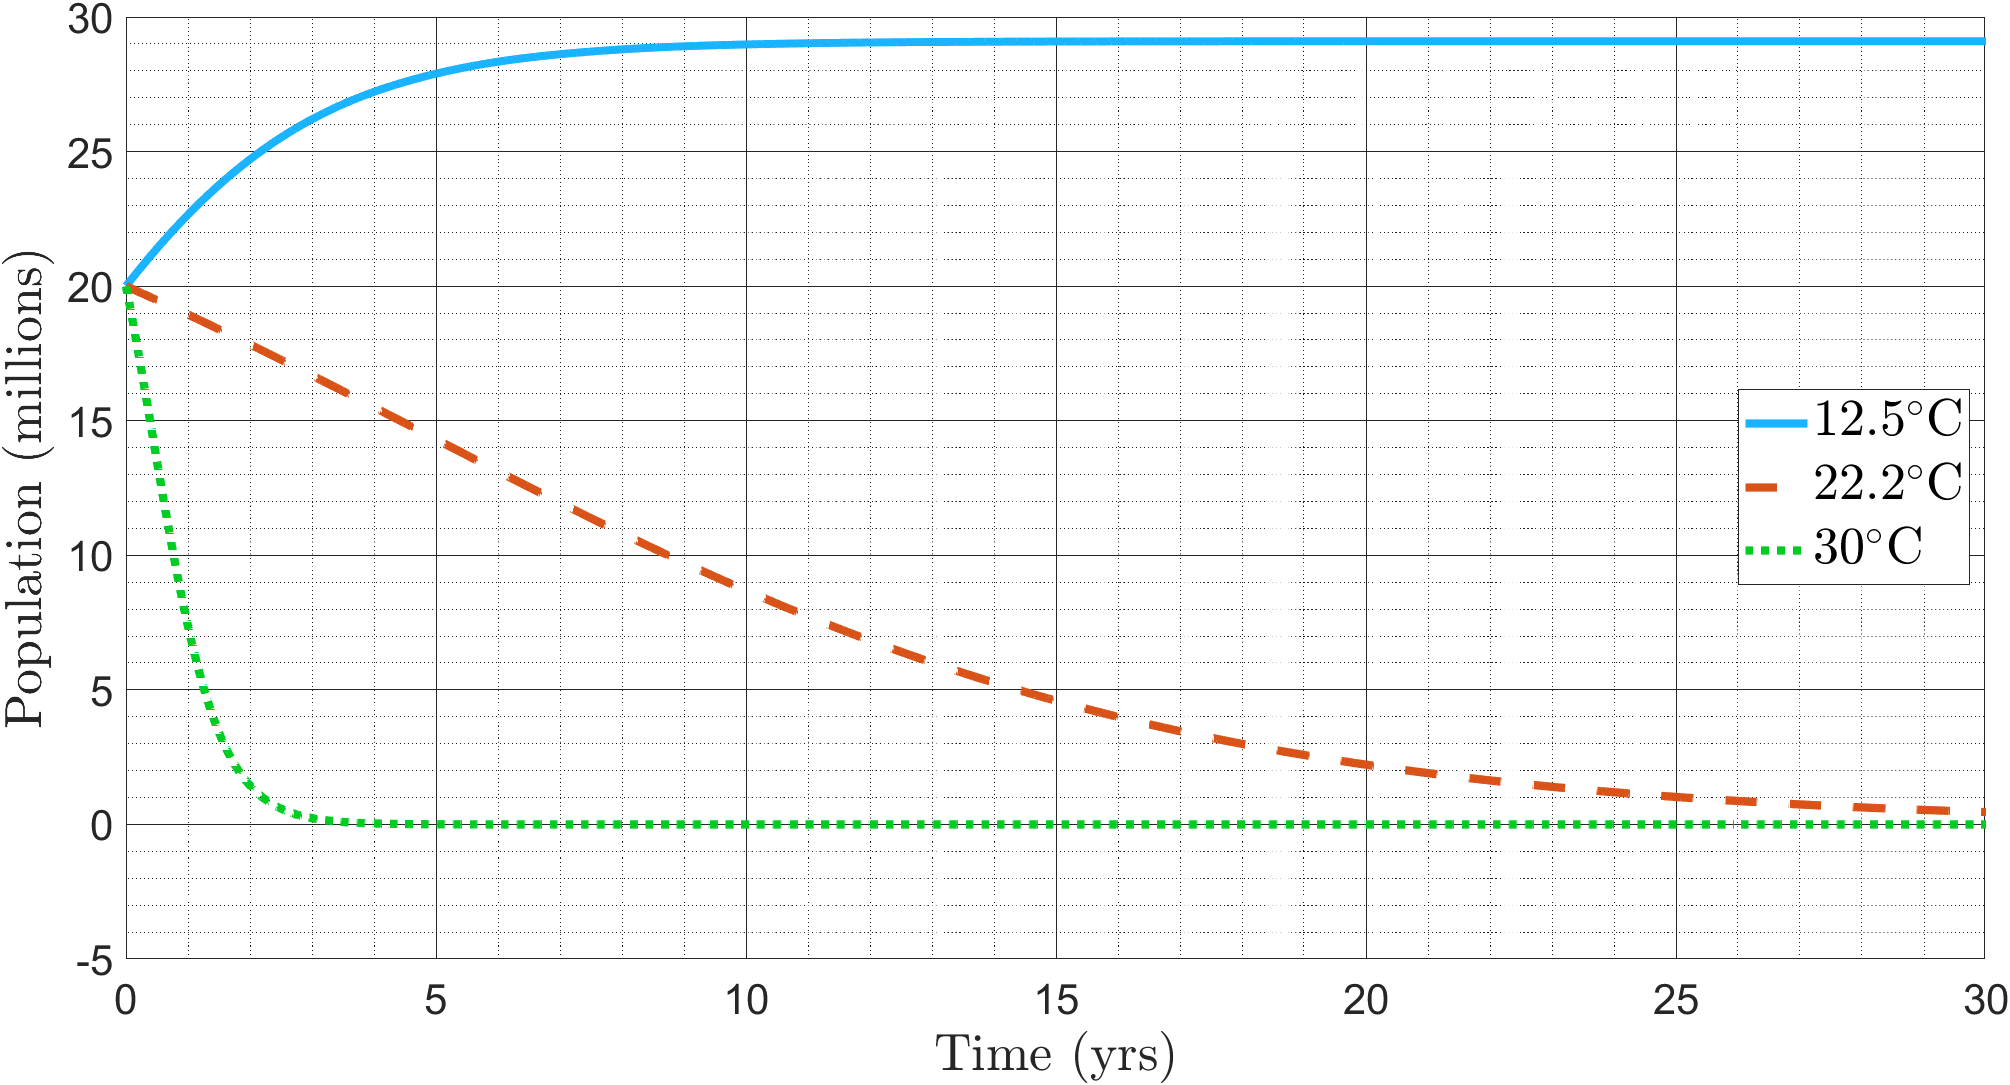
\includegraphics[width=14cm]{Pictures/Salmon Pop/salmon repo model/Salmon at 3 dif temps.png}
    \caption{\singlespacing
    Plot of the salmon logistic growth model using the growth rate function, \equationautorefname~\eqref{eq:salmonlogisticrepo}, at 3 different temperatures.}
    \label{fig:salmonrepocomparison}
\end{figure}
Notice, at the optimal temperature, $T=12.5^{\circ}$C, the curve is the same as in \figureautorefname~\ref{fig:salmnologistic} because $R(12.5) = r_x = 0.47$. 
As the temperature moves further away from the optimal temperature, the reproduction of salmon is negatively affected, resulting in a decay rate, which can be observed in the middle and bottom curves.
When $T=22.2^{\circ}$C the growth rate is $R(22.2) = -0.1641$, which is explains why the population is decreasing over time.
Notice, as the temperature moves drastically far away from the optimal temperature, $T=30^{\circ}$C, the growth rate changes to $R(30)=-1.8698$, causing the population to die off in about 5 years.
By replacing the growth rate of salmon with a function dependent upon temperature, we can see the drastic effects on the salmon population as temperature changes.


\section{Temperature Function Dependent on Time}

The global temperature of the earth has been increasing exponentially over the past 100 years \cite{crowley2000causes}. 
Temperatures are expected to keep increasing for at least the next 30 years unless changes are made now to the emissions of greenhouse gas~\cite{UCAR,university_of_alaska_2016}.
Below is a graph illustrating the annual deviation of global surface temperature from the 20$^{\text{th}}$ century average of 13.9$^{\circ}$C.
\begin{figure}[H]
    \centering
    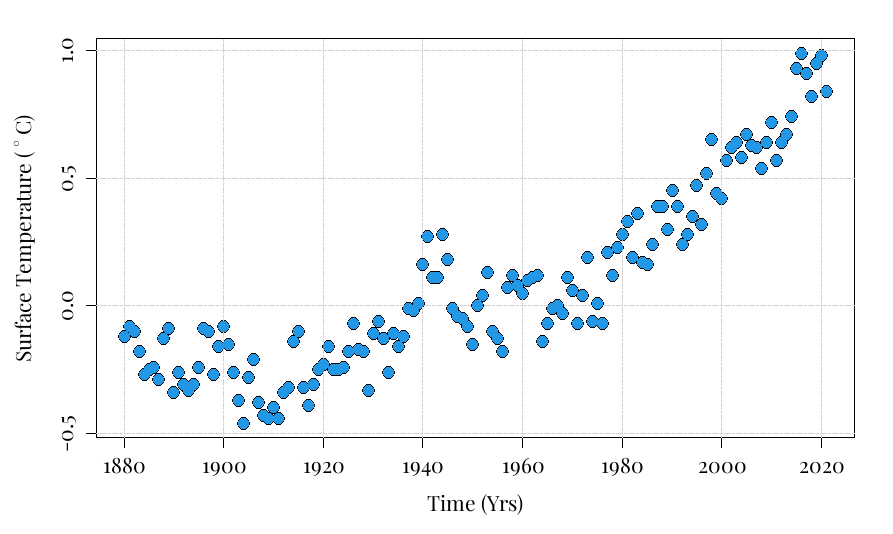
\includegraphics[width=14cm]{LaTeX/Pictures/SST/Global Temp.png}
    \caption{\singlespacing
    Scatter plot of the average annual global temperatures compared to the 20$^{\text{th}}$ century average.}
    \label{fig:noaasurf}
\end{figure}
The data for \figureautorefname~\ref{fig:noaasurf} comes from the National Oceanic and Atmospheric Administration (NOAA)~\cite{NOAA}. 
Any points below 0$^{\circ}$C represent the years when temperatures were less than 13.9$^{\circ}$C, and the points above 0$^{\circ}$C represent the years when temperatures were greater than 13.9$^{\circ}$C.
% Judging from \figureautorefname~\ref{fig:noaasurf}, there seems to be some sense of slowing down after 2010 which aligns with statements made by the EPA, that there has been a recent reduction in the emissions of carbon dioxide \cite{epagreen}.
The earth's surface temperature appears to decrease from 1880 to 1910, then increases exponentially to a little after 1940.
From here, the temperature decreases by approximately $0.05^{\circ}$C entering 1965 before increasing again to the present.
% These dates align closely with the time period of both World Wars, which forced an increase in production.
% We hypothesize that the spike in global surface temperature could be the result of both World Wars.
% The graph above shows that the earth's temperature decreases from 1880 till about 1910 before increasing almost exponentially to the present.
Starting around 1970 to the present, global surface temperatures appear to increase linearly.
While an exponential regression model can be used to fit the data, a quadratic model would seem to work better because of the initial decrease from 1880 to 1910.
The quadratic model would look like
\begin{equation}\label{eq:SSTmodel}
    T(t) = at^2 + bt + c,
\end{equation}
where $a=7.95*10^{-4},\; b=-30.25*10^{-2},\;\text{and } c=287.57$. The response variable, $T(t)$, represents temperature with the units, $^{\circ}$C, that is dependent on time, $t$, expressed in years.
This function seems to fit the data well with the graph below.
\begin{figure}[H]
    \centering
    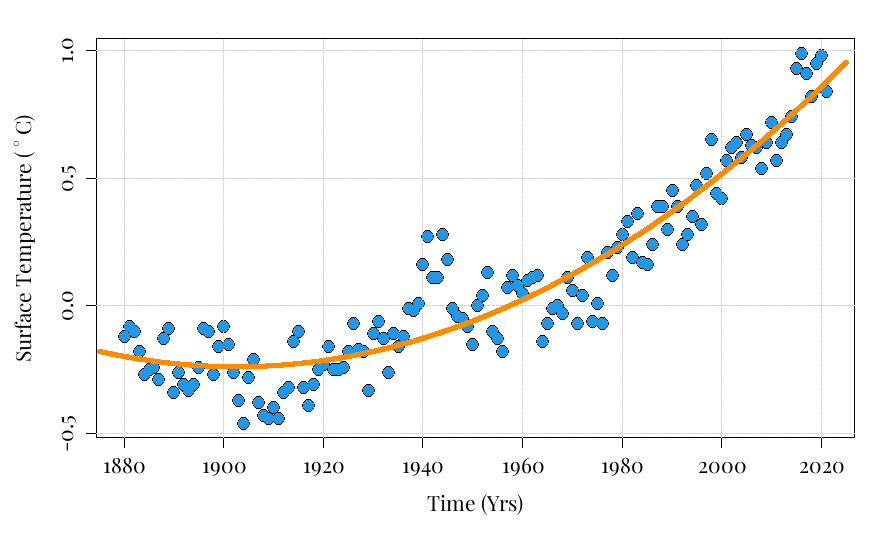
\includegraphics[width=14cm]{Pictures/SST/Global Temp Fit.png}
    \caption{\singlespacing
    Plot of the quadratic function, $T(t)$, on top of the scatter plot given in \figureautorefname~\ref{fig:noaasurf}.}
    \label{fig:polyfitsurf}
\end{figure}
There is a possible issue that should be explored before continuing.
This model projects the change in global  surface temperatures of the earth, but salmon live in the ocean. 
So, designing a model to fit the earth's change in surface temperature over time might not accurately reflect the environmental temperatures of this species.
The National Oceanic and Atmospheric Administration also collect data on the global sea surface temperature over the same time period~\cite{NOAA}.
Below is a graph looking at the global sea surface temperature anomalies with respect to the 20$^{\text{th}}$ century average of 13.9$^{\circ}$C.
\begin{figure}[H]
    \centering
    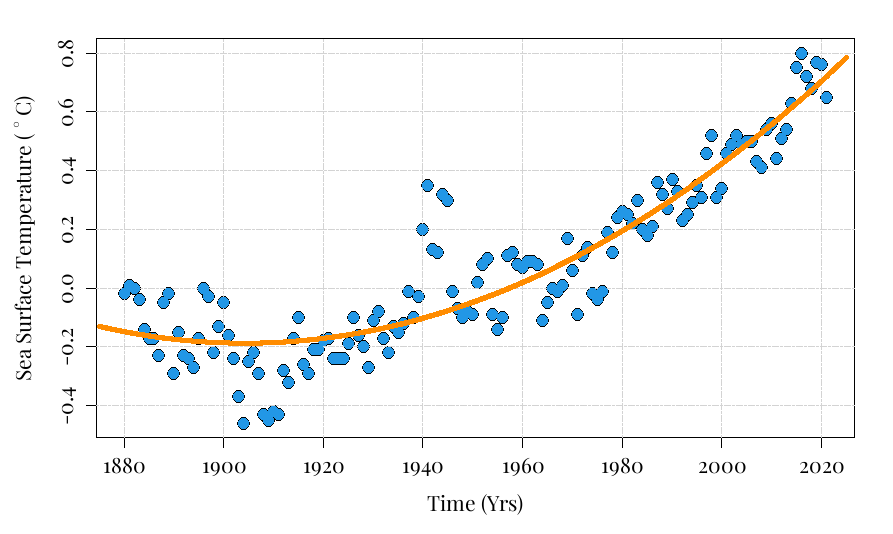
\includegraphics[width=14cm]{Pictures/SST/Global SST Fit.png}
    \caption{\singlespacing
    Scatter plot of the average annual sea surface temperatures compared to the 20$^{\text{th}}$ century average fitted with the quadratic function, $T(t)$, with new coefficients.}
    \label{fig:polyfitSST}
\end{figure}
Since the graph above has a similar trend to \figureautorefname~\ref{fig:noaasurf}, a quadratic model seems to fit this data well.
The new parameters for the quadratic model are, $a=6.67*10^{-5},\; b=-0.25,\; \text{and } c=241.53$.
Looking at \figureautorefname~\ref{fig:polyfitSST} after 1970, the trend appears linear, which means the quadratic equation may not be the best choice for predicting temperature.
Because of this, we will look at sea surface temperatures (SST) after 1970.
Also, Alaska is ranked 40$^{\text{th}}$ in the nation with total greenhouse gas emissions, which may affect that region's SST trend differently than other regions~\cite{adec_2018}.

Alaska has a large number of river streams, but salmon can be seen predominately in the southern parts of Alaska, such as Anchorage, the Kenai Peninsula, near Juneau, and Alaska Peninsula \cite{ADFG}. 
According to the ADFG, salmon swim in these streams from June to September \cite{ADFG}.
Therefore, we sampled water temperature data in these regions during these months to model the change in temperature over time. The data was provided by the United States Geological Survey (USGS)~\cite{usgs_2022}.
When using the USGS database, there are plenty of streams where the Alaskan government was collecting data, but there are a few issues when looking at the data sets for some of the streams~\cite{usgs_2022}.
First, most data sets are a small duration of a few years, which is not enough time to model a trend.
Second, some data sets are missing data for a couple of months every year or even just had big gaps for several years. 
We set criteria for the rivers we wanted to sample; each river needed consistent data for at least 15 years during the months when salmon swim upstream.
In the end, only 5 data sets are usable for analyzing trends over time. 
The 5 streams we use for this analysis are Cooper Creek on the Kenai Peninsula, Kenai River at Cooper Landing, Russell Creek on the Alaska Peninsula, Terror River, just south of the Alaska Peninsula, and Staney Creek which is south of Juneau.
We initially combined the data for each river and calculated the average water temperature per year.
\begin{figure}[H]
    \centering
    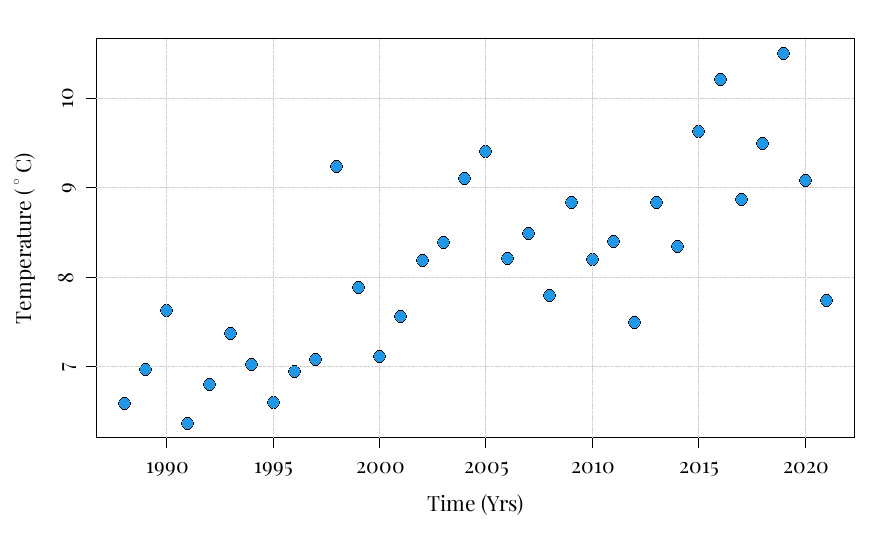
\includegraphics[width=14cm]{Pictures/SST/Alaskan Water Temp.png}
    \caption{\singlespacing
    Scatter plot of the average annual water temperatures during the months of June to September for the combined data of the rivers; Cooper Creek, Kenai River, Russell Creek, Terror River, and Staney Creek. }
    \label{fig:alaskatemp}
\end{figure}
\figureautorefname~\ref{fig:alaskatemp} shows that the trend for the average water temperature per year is fluctuating between increasing and decreasing from 1988 to 2021.
Overall, the data appears to be increasing for the past 33 years.
From \figureautorefname~\ref{fig:alaskatemp}, we can see that, on average, the water temperature is consistently increasing.
This may imply that a linear regression model would fit the data well.
Before fitting the combined river data with a linear model, we have to make sure that each river's change in water temperature over time appears to be increasing linearly.
Below are the plots of each stream fitted with a linear model that closely represents their trend. 
\begin{figure}[H]
    \centering
    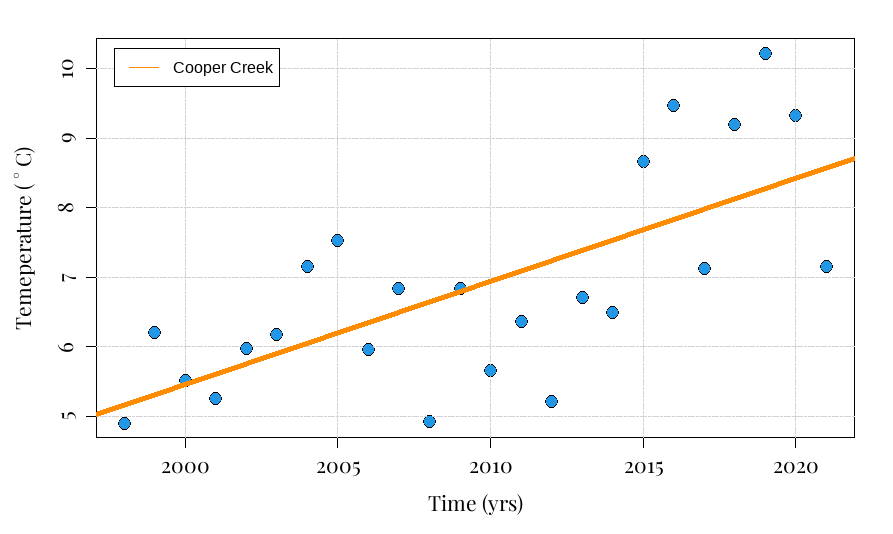
\includegraphics[width=7cm]{Pictures/SST/sst - cooper.png}
    \hfill
    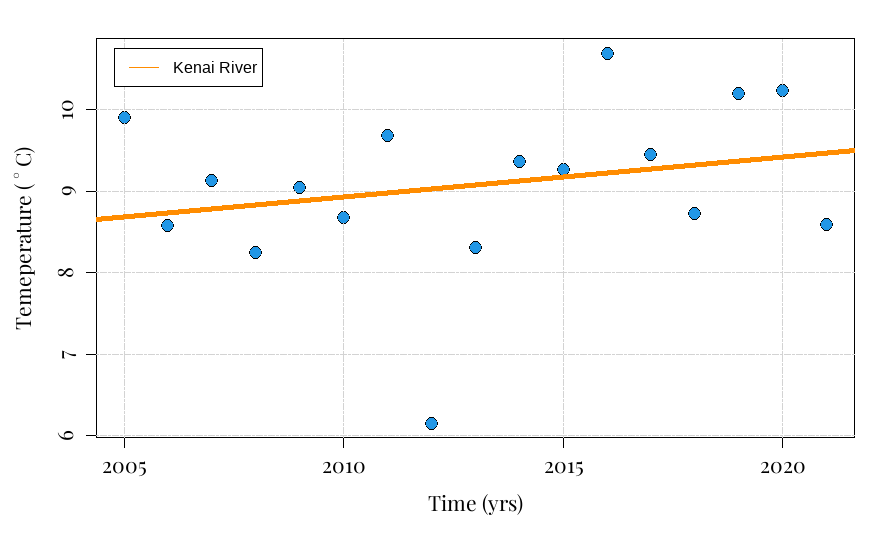
\includegraphics[width=7cm]{Pictures/SST/sst - kenai river.png}
    \\
    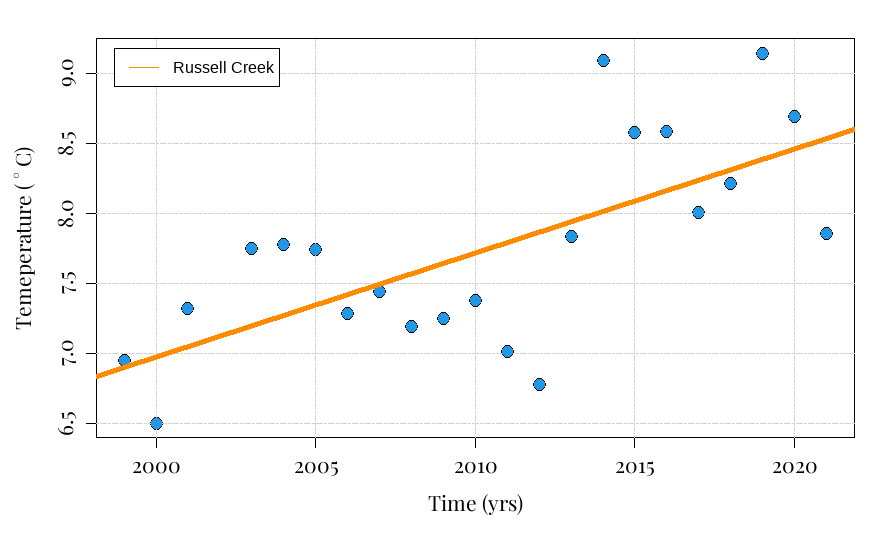
\includegraphics[width=7cm]{Pictures/SST/sst - russell.png}
    \hfill
    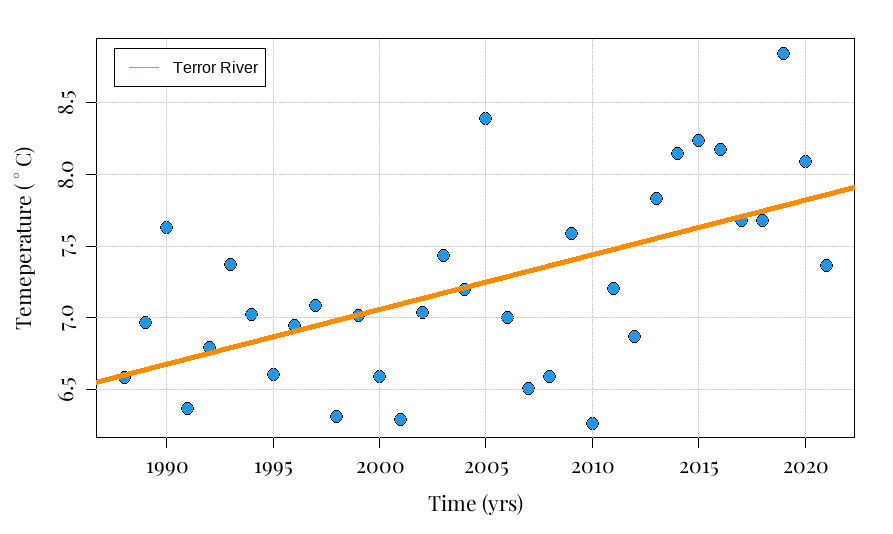
\includegraphics[width=7cm]{Pictures/SST/sst - terror.png}
\end{figure}
\begin{figure}[H]
    \centering
    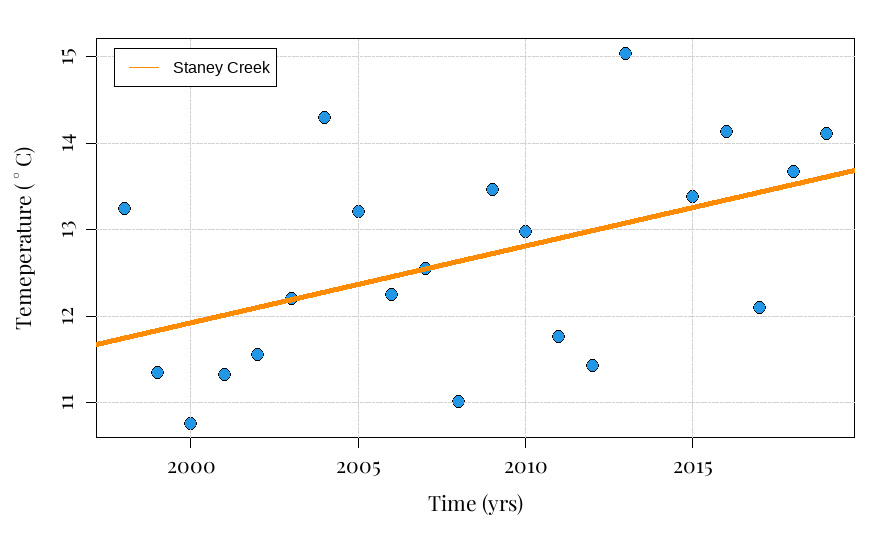
\includegraphics[width=8cm]{Pictures/SST/sst - staney.png}
    \caption{\singlespacing
    Plots of each river's average annual water temperature trend, fitted with a linear model.}\label{fig:sstrivers}
\end{figure}
Notice in \figureautorefname~\ref{fig:sstrivers}, the time span of the recorded water temperatures for some of the rivers are different.
This could cause the combined data used in \figureautorefname~\ref{fig:alaskatemp} to be biased towards rivers with a longer time span.
We can compare the average increase in water temperature for \figureautorefname~\ref{fig:alaskatemp} to the average of the slopes for the rivers in \figureautorefname~\ref{fig:sstrivers}. If the data is biased, we should be able to see it in the comparison.
Each river has a similar trend to the combined data in \figureautorefname~\ref{fig:alaskatemp} with the mean of their slopes representing an average increase in annual water temperature of 0.0797 $^{\circ}$C per year.
When fitting a linear model to \figureautorefname~\ref{fig:alaskatemp} the average increase in water temperature is 0.0803 $^\circ$C per year.
\begin{figure}[H]
    \centering
    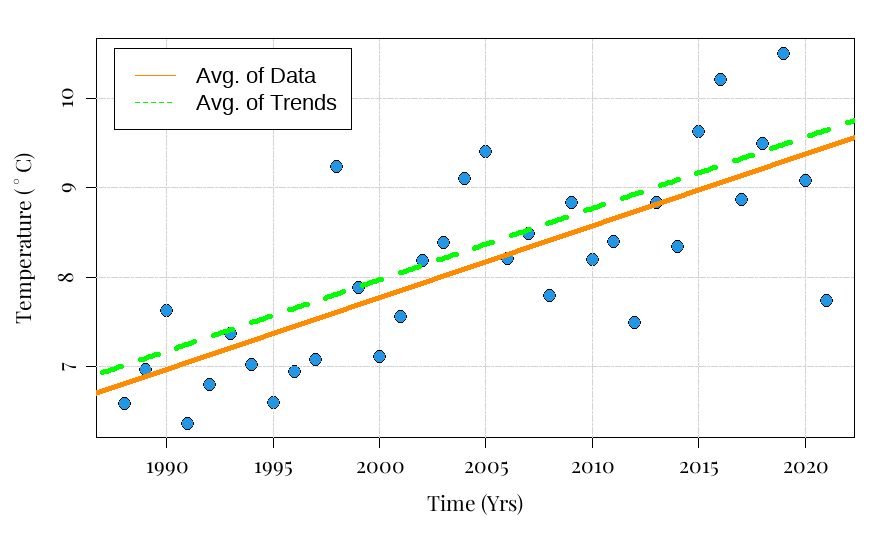
\includegraphics[width=14cm]{LaTeX/Pictures/SST/AlaskaWaterFit.png}
    \caption{\singlespacing
    The solid line represents the average change in annual water temperature of the combined data for the 5 rivers seen in \figureautorefname~\ref{fig:alaskatemp}.
    % the trend of the average water temperature in Alaska for the past 33 years. 
    The dashed line represents the average of the slopes from each river's linear model seen in \figureautorefname~\ref{fig:sstrivers}. 
    % trend for each stream that was sampled in Alaska.
    }
    \label{fig:alaskatempfit}
\end{figure}
The figure above illustrates that for the past 33 years the average change in Alaskan river temperature during the months of salmon spawning migration has a linear growth of approximately 0.08 $^\circ$C per year.
The model for the change in water temperature in Alaska can now be represented as
\begin{equation}\label{eq:sstmodel}
    T(t) = a*t + b,
\end{equation}
with $a=0.08$ and $b = 9.54$. 
The coefficient, $a$, represents the average increase in water temperature over time, and the intercept, $b$, represents 
% the initial water temperature in Alaska about 2000 years ago, and $t$ represents the time in years with an initial starting point 0 B.C. 
% Obviously, the average temperature in Alaskan rivers and creeks 2000 years ago was not $-152.9~^\circ$C, so the linear regression model is only useful for short time periods.
% Thus, letting $b = 9.54$ changes 
the average water temperature for the year 2022.
We will use this model to predict water temperatures in Alaska during the months when salmon migrate to spawning locations.
Now, substituting the function $T(t)$ for the parameter $T$ in \equationautorefname~\eqref{eq:RepoFunLog} gives us
\begin{equation}\label{eq:SalmonRepo}
    \begin{aligned}
        R(T(t)) =\ln\scalebox{1.2}{$\pmb[$}0.32*5*P(T(t))\scalebox{1.2}{$\pmb]$}&= \ln\left(\frac{0.32*5}{1+c(T(t)-T_{opt})^4}\right)\\[.3cm]
        &= \ln\left(\frac{0.32*5}{1+c(at+b-T_{opt})^4}\right).
    \end{aligned}
\end{equation}
Then, substituting in all the parameter values gives the following equation,
\begin{equation}\label{eq:SalmonGrowthTime}
    R(t) = \ln\left(\frac{0.32*5}{1+10^{-4}(0.08t-2.96)^4}\right).
\end{equation}
In \equationautorefname~\eqref{eq:fishexpdif} the growth rate, $r_x$, was revealed after taking the derivative of \equationautorefname~\eqref{eq:fishexp}.
So, by replacing $r_x$ in \equationautorefname~\eqref{eq:fishexp} with $R(t)$ we get
\begin{equation*}
    x(t) = x_0e^{R(t)t}.
\end{equation*}
Then, taking the derivative produces the following,
\begin{equation*}
    \begin{aligned}
        \frac{dx}{dt} &= \pmb[ R(t)+R'(t)t \pmb]x_0e^{R(t)t} = \pmb[ R(t)+R'(t)t \pmb]x,
    \end{aligned}
\end{equation*}
where
\begin{equation}
    R'(t) = \frac{d}{dt}\ln(0.32*5*P(t)) = \frac{P'(t)}{P(t)}.
\end{equation}
As briefly shown in \equationautorefname~\eqref{eq:SalmonRepo}, $P(T)$ from \equationautorefname~\eqref{eq:SurvivalProportionFun} can be rewritten as a function of time using \equationautorefname~\eqref{eq:SSTmodel},
\begin{equation}\label{eq:Repodiff}
    P(t) = \scalebox{1.3}{$\frac{1}{1+10^{-4}(0.08t-2.96)^4}$},\\
\end{equation}
where
\begin{equation}
    P'(t) = \scalebox{1.3}{$\frac{-4*10^{-4}*0.08(0.08t-2.96)^3}{\left(1+10^{-4}(0.08t-2.96)^4\right)^2}$}.\\
\end{equation}
So, the growth rate function can now be written as
\begin{equation}
    G(t) = \ln\left(\frac{0.32*5}{1+10^{-4}(0.08t-2.96)^4}\right) - \scalebox{1.3}{$\frac{4*10^{-4}*0.08t(0.08t-2.96)^3}{1+10^{-4}(0.08t-2.96)^4}$},
\end{equation}
or in a more simplified form,
\begin{equation}\label{eq:GrowthRate}
    G(t) = R(t) + \frac{P'(t)t}{P(t)}.
\end{equation}
To better understand what the growth rate function is doing, we graph the function below.
\begin{figure}[H]
    \centering
    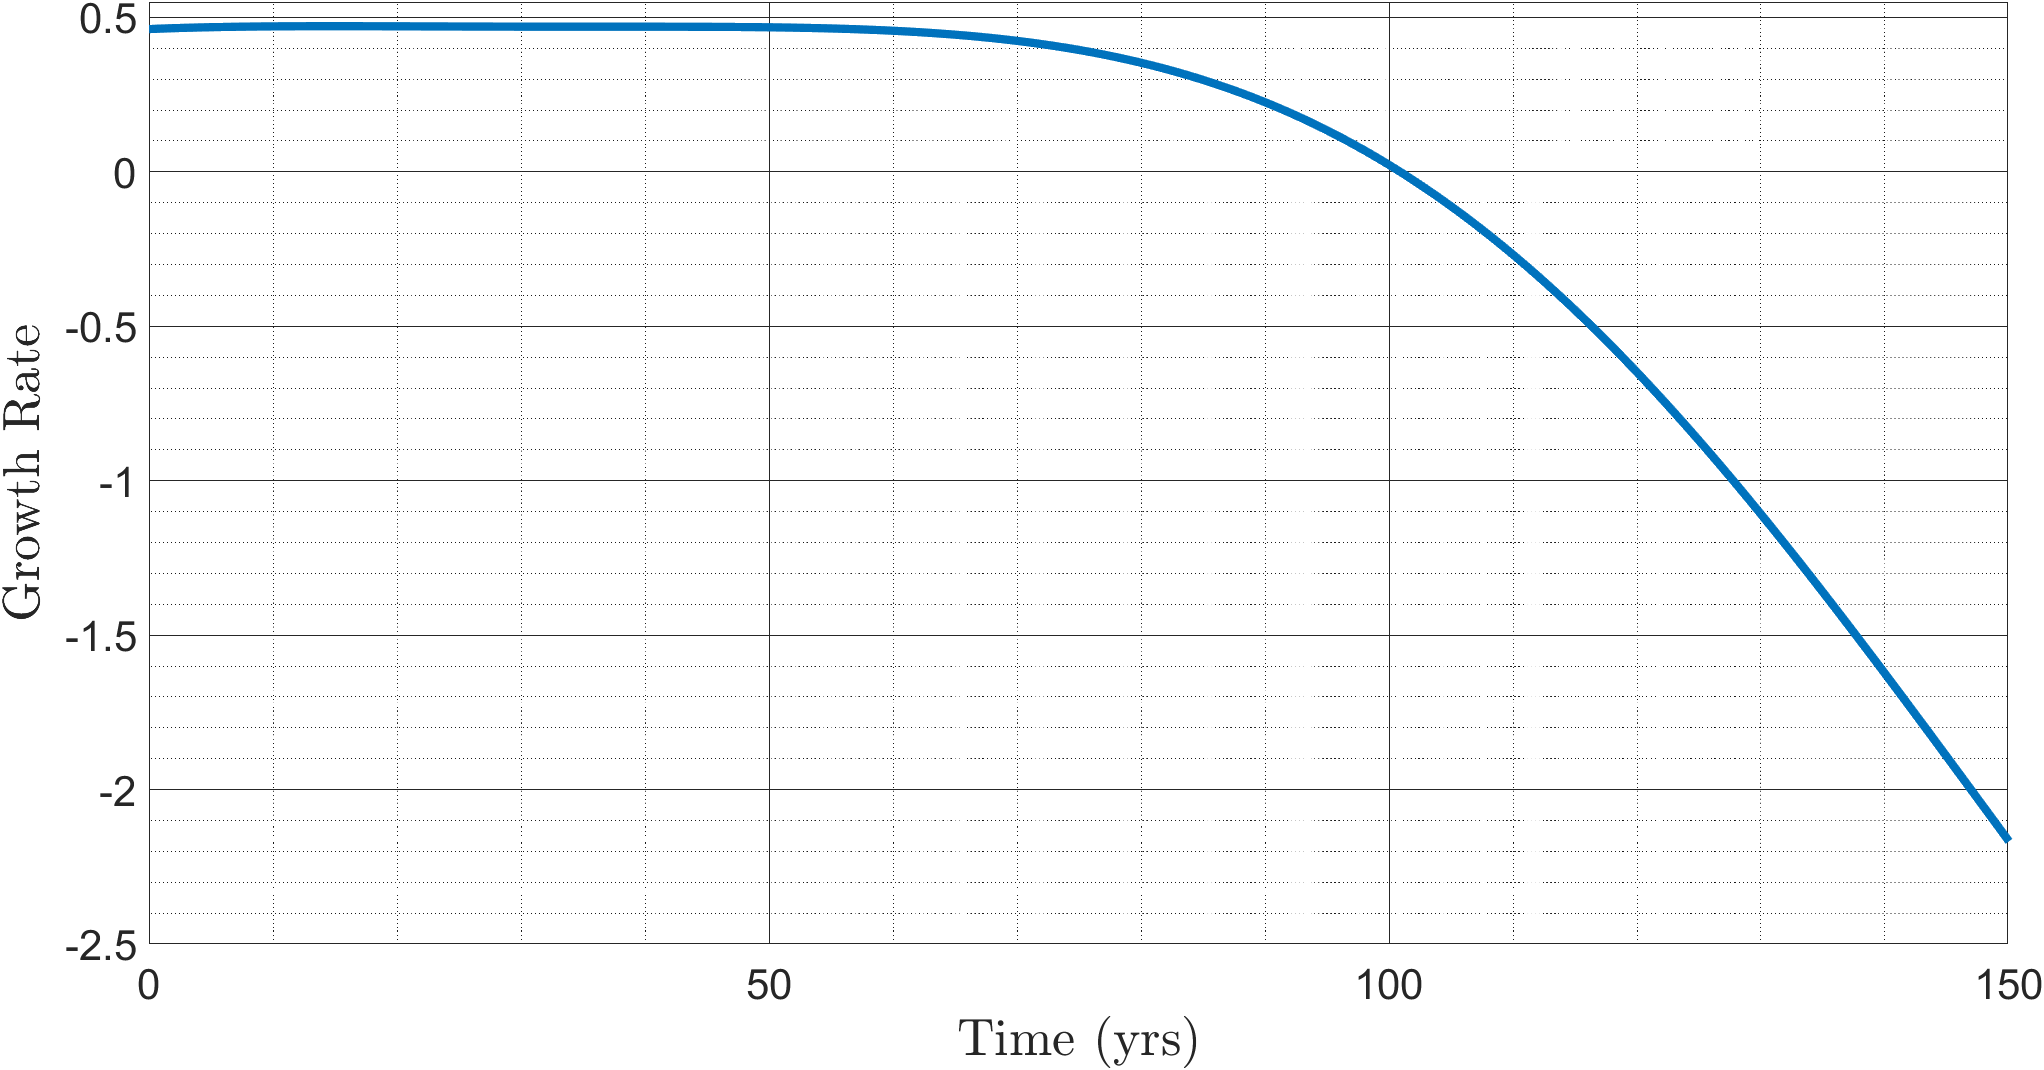
\includegraphics[width=14cm]{Pictures/Salmon Pop/GrowthRateFun.png}
    \caption{\singlespacing
    Plot of the growth rate function, \equationautorefname~\eqref{eq:GrowthRate}, over a time span of 150 years.}
    \label{fig:GrowthRateFunction}
\end{figure}
We can see in the figure above that the growth rate remains positive for approximately the first 100 years. 
After this, the growth rate becomes negative indefinitely.
Now, as shown below, we can substitute the above growth rate function into \equationautorefname~\eqref{eq:salmonlogisticrepo}.
\begin{equation}\label{eq:SalmonLogTime}
    \frac{dx}{dt} = G(t)x\left(1-\frac{x}{K_x}\right).
\end{equation}
Since the model for the salmon population is now dependent on time, it becomes a non-autonomous ordinary differential equation. When comparing this model to \equationautorefname~\eqref{eq:salmonlogisticrepo}, the below figure is produced.
\begin{figure}[H]
    \centering
    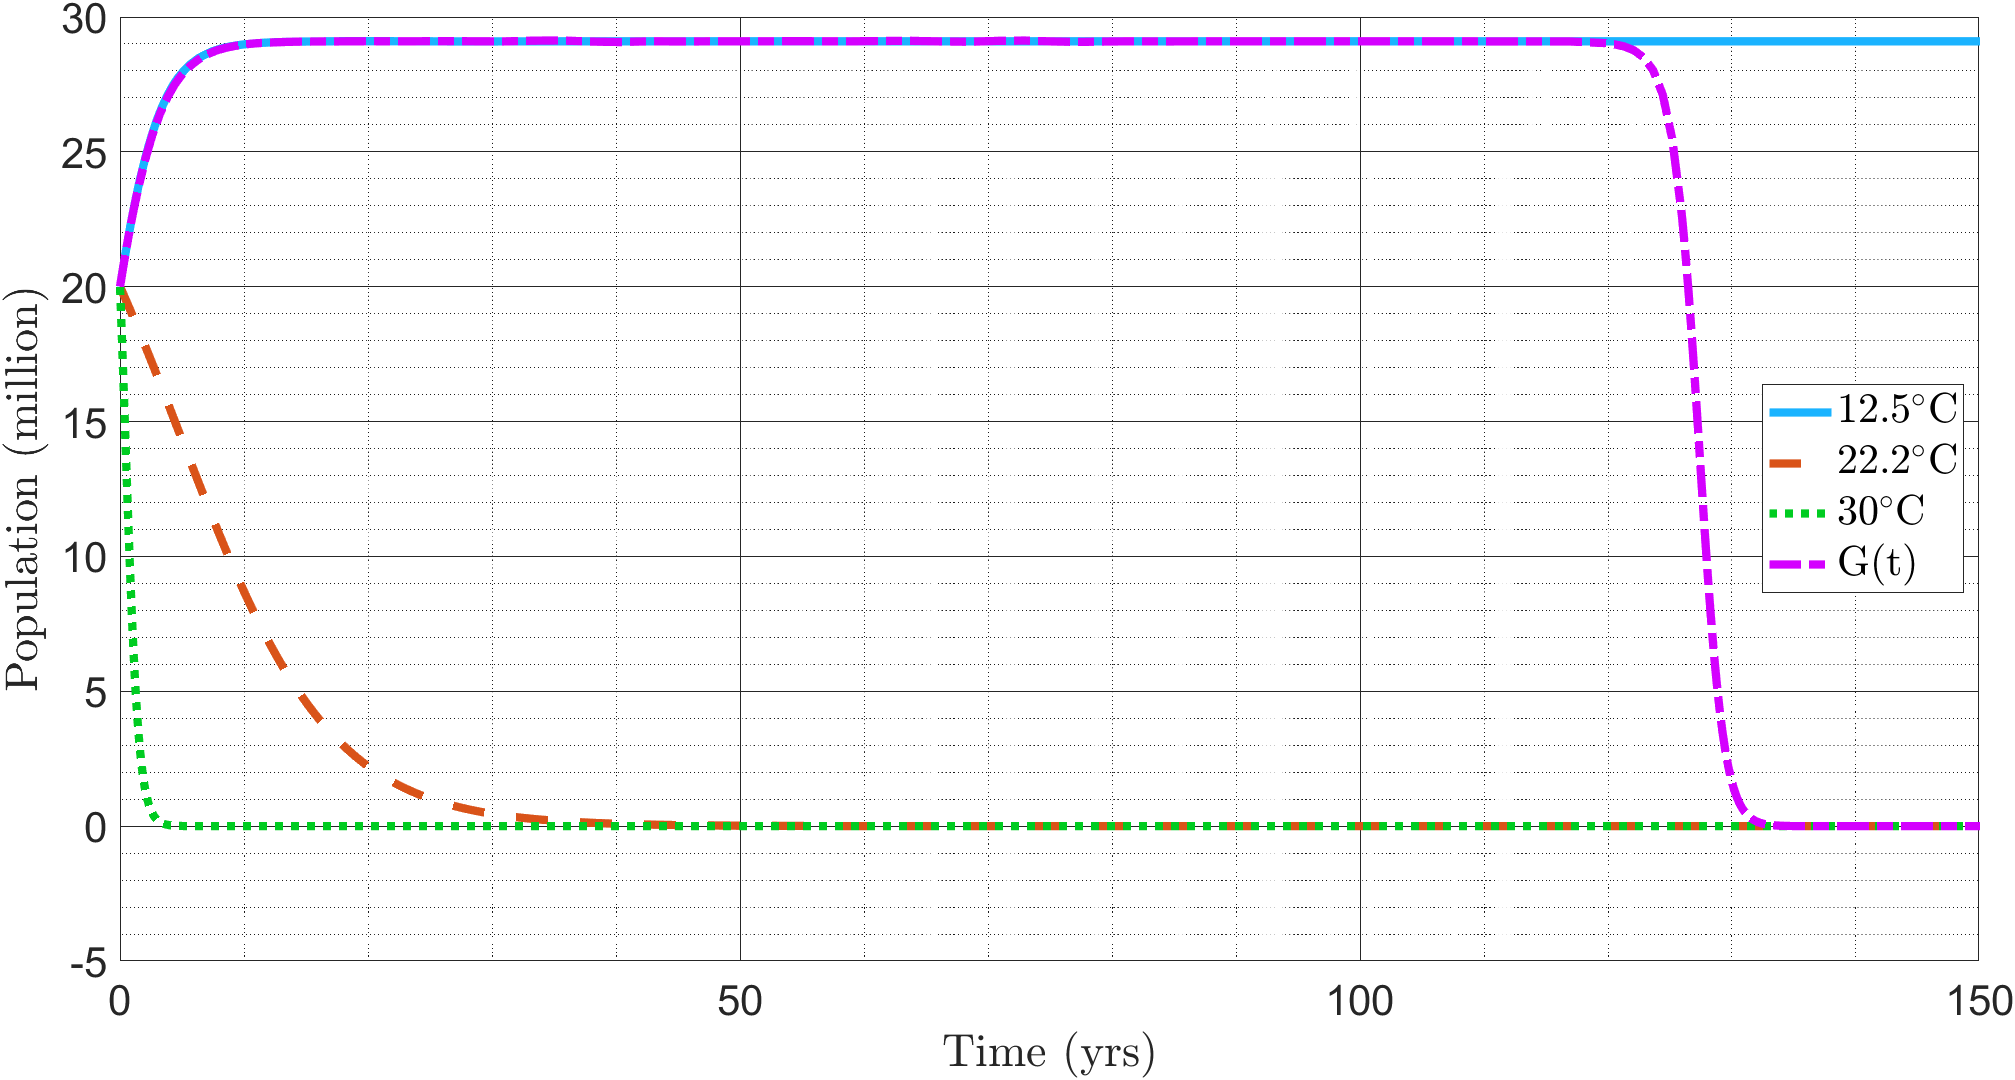
\includegraphics[width=14cm]{Pictures/Salmon Pop/salmon repo model/SalmonWithRepoFun.png}
    \caption{\singlespacing
    Solutions to the autonomous system for some values of water temperature $T$, and the non-autonomous system as a function of time.
    % This figure plots the solutions to \equationautorefname~\eqref{eq:SalmonLogTime}onto \figureautorefname~\ref{fig:salmnologistic}. Also, compared to \figureautorefname~\ref{fig:salmnologistic} the x-axis limits are expanded to illustrate the decline in the salmon population as time gets large.
    }
    \label{fig:SalmonWithRepoFun}
\end{figure}
Using the \textbf{vpasolve} function in MATLAB, we found that in approximately 101 years, the growth rate will change from positive to negative, which is the beginning of the population's descent.
When substituting $t=101$ into \equationautorefname~\eqref{eq:sstmodel}, we get $T(101) = 17.62^{\circ}$C.
This temperature can be denoted as our inflection temperature for the salmon population.
\figureautorefname~\ref{fig:SalmonWithRepoFun} suggests that the water temperature will be too hot for the salmon population in the future, resulting in their death or regional extinction.




\section{Conclusion}

In this chapter, we proposed a salmon growth rate function that depends on water temperature.
We used river temperature data from the United States Geological Survey (USGS) to design a function that models the increase in Alaskan river temperature over time, which can be seen below,
\begin{equation*}
    T(t) = a*t + b,
\end{equation*}
where $a=0.08$, and $b=9.54$.
Also, $t=0$ represents the current year, 2022.
We then make the growth rate function dependent on time by replacing the temperature parameter $T$ with the temperature function, as shown bellow,
\begin{equation*}
    \begin{array}{ll}
        G(t) &= R(t) + \scalebox{1.2}{$\frac{P'(t)t}{P(t)}$} \\[.2cm]
         &= \ln\left(\scalebox{1.2}{$\frac{0.32*5}{1+10^{-4}(0.08t-2.96)^4}$}\right) - \scalebox{1.2}{$\frac{4*10^{-4}*0.08t(0.08t-2.96)^3}{1+10^{-4}(0.08t-2.96)^4}$}.
    \end{array}
\end{equation*}
Lastly, we replaced this new growth rate function with the growth rate parameter in the original logistic model, \equationautorefname~\eqref{eq:fishlogistic}, and compare its results.
We found that after approximately 100 years, the salmon population will begin to decline and eventually die off or migrate elsewhere.
In the next chapter, we will examine the effect of interaction between the brown bear and salmon species.
We will compare the results of the interaction with and without the growth rate function.

\chapter{Interaction Between Species}

% Many population growth models use variations of the Verhulst logistic growth equation to simulate the population growth of living organisms.
% James Wallace and Anastasios Tsoularis review different variations of the logistic growth equation in their article, ``Analysis of logistic growth models''~\cite{tsoularis2002analysis}.
% In this thesis, we will use variations of the logistic growth model to describe the populations of pacific salmon and Alaskan brown bears.

In this chapter, we introduce simple logistic growth models for the salmon and brown bear species.
Using information from the Alaskan Department of Fish and Game, we estimate a growth rate parameter for the salmon population.
Then, we choose the carrying capacity parameter by calculating the maximum volume of salmon for any given inshore run\footnote{Inshore runs are when salmon migrate back from the sea to spawn.} in Bristol Bay, Alaska.
We find 3 growth rates from 3 articles for the Alaskan brown bears and calculate their mean, which we use to represent their growth rate parameter~\cite{daele2010management,mclellan1989,mclellan1996}.
Also, for this model, we estimate the carrying capacity based on information from the Alaskan Department of Fish and Game (ADFG)~\cite{ADFG}.



% we begin by creating an appropriate logistic growth model for the brown bear population using growth rates from a few scholarly articles and approximating a carrying capacity from the Alaskan Department of Fish and Game (ADFG). 
% Next, Volhulst’s logistic growth model will illustrate the salmon population using information from the ADFG to achieve a growth rate. 
% Also, the carrying capacity is revealed through the relationship between salmon run size and their average weight during their run. 
% Finally, the chapter briefly compares the two models and introduces the concept of creating a variation of the logistic model that incorporates the aspect of climate change.

\section{Lotka-Volterra Equations}

In nature, most animals share their environment, which sometimes causes species to interact, like salmon and brown bears. 
This relationship can be portrayed by incorporating interaction terms into each species' population equation.
% The interaction terms depend on both species’ populations and use positive real parameters to describe the effect of one species on the other.
The Lotka-Volterra model, also referred to as the predator-prey model, is a simple system of two nonlinear ordinary differential equations that utilize interaction terms to imitate the relationship between two species~\cite{anisiu2014lotka},
\begin{equation}\label{eq:lotkavoltera}
    \begin{aligned}
        \frac{dx}{dt} & = \alpha x - \beta xy,\\
        \frac{dy}{dt} & = \delta xy - \gamma y.
    \end{aligned}
\end{equation}
Consider $x$ as the prey, $y$ as the predator, and $\alpha$, $\beta$, $\delta$, $\gamma$ are positive real parameters that describe the interaction of the two species. 
Also, $\displaystyle \frac{dx}{dt}$ and $\displaystyle \frac{dy}{dt}$ represent each species' instantaneous population rate of change. 
The interaction term for species $x$ is subtracted from the exponential growth component, $\alpha x$, to describe that the instantaneous growth rate of species $x$ will decrease as $y$ increases. The opposite effect happens to species $y$ because its interaction term is added instead of subtracted.
The author of ``US Nobel laureates: Logistic growth versus Volterra–Lotka'', Theodore Modis, developed a competitive predator-prey model that implements logistic growth into the Lotka-Volterra equations,
\begin{equation}\label{eq:modislotkavoltera}
    \begin{aligned}
    \frac{dx}{dt} &= a_xx - b_xx^2 + c_{xy}xy,\\
    \frac{dy}{dt} &= a_yy - b_yy^2 + c_{yx}xy,
    \end{aligned}
\end{equation}
where $a_{x}$, $a_{y}$, $b_{x}$, $b_{y}$, $c_{xy}$ and $c_{yx}$ are real parameters that describe the interaction of the two species~\cite{modis2011us}.



% This model is describing two species who have an interaction with themselves, which is the logistic equation, and an interaction with each other, which is the interaction terms added at the end of each equation.

% The fundamentals of each of these equations will be used in the construction of our model. 
% The Lotka-Volterra will assist in the illustrating interaction between species while the logistic equations will be used to describe the environmental limits of each species.




\section{Introducing Interaction}

Currently, we have constructed models for both species that represent their populations without the influence of each other. 
% The models found in \equationautorefname~\eqref{eq:LogBear} and \equationautorefname~\eqref{eq:salmonlogisticrepo} are designed to individually represent the species' populations.
% This means that the outcome of one species does not affect the other.
By including interaction terms for both models, we can simulate a trade-off of environmental resources, as we would see in the real world.
First, we use a variation of Theodore Modis' model, \equationautorefname~\eqref{eq:modislotkavoltera}, to introduce interaction between the brown bears and salmon when both species are unaffected by climate change,
\begin{equation}\label{eq:AutonomousSystemODEs}
    \begin{aligned}
    \frac{dx}{dt} &=r_xx\left(1-\frac{x}{K_x}\right) - c_{xy}xy,\\[.4cm]
    \frac{dy}{dt} &=r_yy\left(1-\frac{y}{K_y}\right) + c_{yx}xy,
    \end{aligned}
\end{equation}
where $r_x = \ln(0.32*5),\ r_y=0.059,$ and $c_{xy},\;c_{yx}>0$. \equationautorefname s~\eqref{eq:fishlogistic} and~\eqref{eq:LogBear} represent the base models of the above system of differential equations where both species are unaffected by climate change.
Notice, for the salmon ODE, we subtract its interaction term, but for the brown bears, we add its interaction term.
We do this because the salmon population should have a negative consequence when there is an increase in brown bears.
In contrast, brown bears should be rewarded when their food source increases.
The interaction parameters alter the effect of the carrying capacity, so we change $K_x = 15$ and $K_y=5$ as a vague measure of their environmental limits.
We can rewrite the system of equations in a similar form to Theodore Modis' model, as shown below,
\begin{equation}
    \begin{aligned}
    \frac{dx}{dt} &= r_xx -\frac{r_xx^2}{K_x} - c_{xy}xy,\\[.4cm]
    \frac{dy}{dt} &=r_yy -\frac{r_yy^2}{K_y} + c_{yx}xy.
    \end{aligned}
\end{equation}
Then, substituting $ a_x = r_x$, $\displaystyle b_x = \frac{r_x}{K_x}$, $a_y = r_y$, and $\displaystyle b_y = \frac{r_y}{K_y}$ we get
\begin{equation}\label{eq:AutonomousSystemODEsModis}
    \begin{aligned}
    \frac{dx}{dt} &= a_xx - b_xx^2 - c_{xy}xy,\\
    \frac{dy}{dt} &= a_yy - b_yy^2 + c_{yx}xy.
    \end{aligned}
\end{equation}
Condensing the model reduces the number of parameters in each equation, which makes the model and any operations done to the model more readable and interpretable.
In the next section, we determine how different values for the parameters, $c_{xy}$ and $c_{yx}$, control the stability of the populations near their critical points.


\section{Critical Points and Their Stability}

% Before, finding the critical points of \equationautorefname~\eqref{eq:AutonomousSystemODEs}, we fix the parameter, $T$, to the optimal temperature, $12.5^{\circ}$C, eliminating the effect of temperature on the salmon population.
% We can also rewrite the equations in a similar form to Theodore Modis' model, as shown below,
% \begin{equation}
%     \begin{aligned}
%     \frac{dx}{dt} &= R(T_{opt})x -\frac{R(T_{opt})x^2}{K_x} - c_{xy}xy,\\[.4cm]
%     \frac{dy}{dt} &=r_yy -\frac{r_yy^2}{K_y} + c_{yx}xy.
%     \end{aligned}
% \end{equation}
% Then, substituting $ a_x = R(T_{opt})=0.47$, $\displaystyle b_x = \frac{R(T_{opt})}{K_x}=0.0313$, $a_y = r_y=0.044$, and $\displaystyle b_y = \frac{r_y}{K_y}=.0088$ we get
% \begin{equation}\label{eq:AutonomousSystemODEsModis}
%     \begin{aligned}
%     \frac{dx}{dt} &= a_xx - b_xx^2 - c_{xy}xy,\\
%     \frac{dy}{dt} &= a_yy - b_yy^2 + c_{yx}xy.
%     \end{aligned}
% \end{equation}
We find the critical points by setting the rate functions in \equationautorefname~\eqref{eq:AutonomousSystemODEsModis} to 0,
\begin{equation*}
    \begin{aligned}
    0 &= x(a_x - b_xx - c_{xy}y),\\
    0 &= y(a_y - b_yy + c_{yx}x).
    \end{aligned}
\end{equation*}
Then, we solve for $x$ and $y$ to get the following critical points;
\begin{equation*}
    \begin{array}{llll}
         x^*_1 = 0, &&& y^*_1 = 0,  \\[.2cm]
         x^*_2 = \scalebox{1.3}{$\frac{a_x}{b_x}$}= K_x,&&& y^*_2 = 0,\\[.2cm]
         x^*_3 = 0, &&& y^*_3 = \scalebox{1.3}{$\frac{a_y}{b_y}$}=K_y,\\[.2cm]
         x^*_4 = \scalebox{1.3}{$\frac{a_xb_y-c_{xy}a_y}{c_{xy}c_{yx}+b_xb_y}$}, &&& y^*_4 = \scalebox{1.3}{$\frac{a_xc_{yx}+b_xa_y}{c_{xy}c_{yx}+b_xb_y}$}.
    \end{array}
\end{equation*}
We can determine the stability at each of the above critical points by finding the eigenvalues of our model, \equationautorefname~\eqref{eq:AutonomousSystemODEsModis}~\cite{roussel2019stability}.
We begin by constructing the Jacobian matrix,
\begin{equation}\label{eq:Jacobian}
    J_{(x,y)} =
    \begin{pmatrix}
        a_x - 2b_xx -c_{xy}y & -c_{xy}x\\
        c_{yx}y & a_y - 2b_yy + c_{yx}x
    \end{pmatrix}.
\end{equation}
Then, we derive the characteristic polynomial,
\begin{align}
\begin{split}\label{eq:CharacteristicEq}\displaystyle
    \text{det}(J_{(x,y)}-\lambda I) = \lambda^2 - \pmb{\big[}\; (a_x - 2b_xx -c_{xy}y) + (a_y - 2b_yy + c_{yx})\;\pmb{\big]}\lambda\\
    + \pmb{\big[}\; (a_x - 2b_xx -c_{xy}y)(a_y - 2b_yy + c_{yx}) + c_{xy}xc_{yx}y\;\pmb{\big]}.
\end{split}
\end{align}
Note that the trace and determinant of the Jacobian matrix are
\begin{equation*}
    \begin{array}{ll}
         \mathrm{T} &= \text{tr}(J_{(x,y)}) = (a_x - 2b_xx -c_{xy}y) + (a_y - 2b_yy + c_{yx}),
         \\
         \mathrm{D} &= \text{det}(J_{(x,y)}) = (a_x - 2b_xx -c_{xy}y)(a_y - 2b_yy + c_{yx}) + c_{xy}xc_{yx}y.
    \end{array}
\end{equation*}
So, substituting the above variables in \equationautorefname~\eqref{eq:CharacteristicEq} produces
\begin{equation*}
    \text{det}(J_{(x,y)}-\lambda I) = \lambda^2 - \mathrm{T}\lambda + \mathrm{D}.
\end{equation*}
Now, solving for our eigenvalues, $\lambda$, gives the below equation,
\begin{equation*}
    \lambda = \frac{\mathrm{T} \pm \sqrt{\mathrm{T}^2 - 4\mathrm{D}}}{2}.
\end{equation*}
Using the equation above, we can determine the signs and potentially the numeric values of the real and imaginary parts of the eigenvalues for each critical point.
Starting with the first critical point, $(0,\;0)$, we get
\begin{equation*}
    \begin{array}{l}
         \mathrm{T}= a_x+a_y, \\
         \mathrm{T}^2 - 4\mathrm{D}= (a_x-a_y)^2 .
    \end{array}
\end{equation*}
So, substituting in the values for $a_x$ and $a_y$, we get
\begin{equation*}
    \begin{array}{l}
         \mathrm{T} = \ln(0.32*5) + 0.059 \approx 0.529,  \\
         \mathrm{T}^2-4\mathrm{D} = (\ln(0.32*5)-0.059)^2 \approx 0.169.
    \end{array}
\end{equation*}
Since $\mathrm{T}\approx 0.529 > \sqrt{\mathrm{T}^2-4\mathrm{D}} \approx 0.411$, both eigenvalues are positive real values, which implies that the first critical point is an unstable node. Now, for the second critical point, $\displaystyle\left(\frac{a_x}{b_x},\;0\right)$, we get
\begin{equation*}
    \begin{array}{l}
        \mathrm{T}= a_x \left(\scalebox{1.3}{$\frac{c_{yx}}{b_x}$}-1\right)+a_y, \\[.2cm]
        \mathrm{T}^2 - 4\mathrm{D}= \scalebox{1.3}{$\frac{(a_x (b_x+c_{yx})+a_y b_x)^2}{b_x^2}$},
    \end{array}
\end{equation*}
where the stability is dependent on $c_{yx}$.
Because the value for the discriminant is squared, it is always positive, which implies that the eigenvalues are real.
When we substitute the parameters, $a_x,\;b_x,$ and $a_y$ for their numeric values, we get the following criterion;
\begin{equation*}
    \begin{array}{l}
        \mathrm{T}+\sqrt{\mathrm{T}^2-4\mathrm{D}}>0,  \\
         \mathrm{T}-\sqrt{\mathrm{T}^2-4\mathrm{D}}<0.
    \end{array}
\end{equation*}
This implies that one eigenvalue is positive while the other is negative, which makes $\displaystyle\left(\frac{a_x}{b_x},\;0\right)$ a saddle point.
% for any $c_{yx}>0$. 
Now, looking at the third critical point, $\displaystyle\left(0,\;\frac{a_y}{b_y}\right)$, the trace and discriminant are;
\begin{equation*}
    \begin{array}{l}
        \mathrm{T}= a_x-\scalebox{1.3}{$\frac{a_y (b_y+c_{xy})}{b_y}$}, \\[.2cm]
        \mathrm{T}^2 - 4\mathrm{D}= \scalebox{1.3}{$\frac{(a_x b_y+a_y (b_y-c_{xy}))^2}{b_y^2}$},
    \end{array}
\end{equation*}
where the stability is now dependent on $c_{xy}$.
Just like for the last critical point, the discriminant is always positive, which implies the eigenvalues are also real.
Then, we substitute the values for, $a_x,\;a_y,$ and $b_y$, into the above equations to get the criterion below;
\begin{equation*}
    \begin{array}{l}
        \mathrm{T}+\sqrt{\mathrm{T}^2-4\mathrm{D}}>0\ \ \text{when \ } c_{xy}<0.094,  \\
        \mathrm{T}-\sqrt{\mathrm{T}^2-4\mathrm{D}}<0.
    \end{array}
\end{equation*}
From the signs of the eigenvalues, we determine that $\displaystyle\left(0,\;\frac{a_y}{b_y}\right)$ is a saddle point when $c_{xy}<0.094$, and a stable node when $c_{xy}>0.094$.
Lastly, with the critical point,
\begin{equation*}
    \left(x_4^*,\;y_4^*\right) = \left(\scalebox{1.3}{$\frac{a_xb_y-c_{xy}a_y}{c_{xy}c_{yx}+b_xb_y}$},\; \scalebox{1.3}{$\frac{a_xc_{yx}+b_xa_y}{c_{xy}c_{yx}+b_xb_y}$}\right),
\end{equation*}
we get the following trace and discriminant equations;
\begin{equation*}
    \begin{array}{l}
        \mathrm{T}= \scalebox{1.3}{$\frac{a_y b_x (c_{xy}-b_y)-a_x b_y (b_x+c_{yx})}{b_x b_y+c_{xy} c_{yx}}$}, \\[.3cm]
        \begin{aligned}
            \mathrm{T}^2 - 4\mathrm{D}=& \scalebox{1.3}{$\frac{(a_y b_x (c_{xy}-b_y)-a_x b_y (b_x+c_{yx}))^2}{(b_x b_y+c_{xy} c_{yx})^2}$}\\[.2cm]
            &- \scalebox{1.3}{$\frac{4 (a_x c_{yx}+a_y b_x) (a_x b_y-a_y c_{xy}) (b_x b_y+c_{xy} c_{yx})}{(b_x b_y+c_{xy} c_{yx})^2}$},
        \end{aligned}
    \end{array}
\end{equation*}
where the stability is dependent on parameters, $c_{xy}$ and $c_{yx}$.
Since the other critical points contain one or more species with a population size of 0, we construct the following constraints for the critical point;
\begin{equation*}
    x_4^* = \scalebox{1.3}{$\frac{a_xb_y-c_{xy}a_y}{c_{xy}c_{yx}+b_xb_y}$}>0,\quad \text{and}\quad y_4^* = \scalebox{1.3}{$\frac{a_xc_{yx}+b_xa_y}{c_{xy}c_{yx}+b_xb_y}$}>0,
\end{equation*}
which eliminates the chance of repeating any of the first 3 critical points.
From the above constraint, we create the below criterion for $c_{xy}$ and $c_{yx}$;
\begin{equation*}
\begin{array}{c}
     0<c_{xy} < \scalebox{1.3}{$\frac{a_xb_y}{a_y}$}, \\[.1cm]
     c_{yx} > -\scalebox{1.3}{$\frac{b_xa_y}{a_x}$}.
\end{array}
\end{equation*}
Since $a_x,\;b_x,\;a_y>0$, the criterion changes to
\begin{equation*}
\begin{array}{c}
     0<c_{xy} < \scalebox{1.3}{$\frac{a_xb_y}{a_y}$} \approx 0.094, \\
     c_{yx} > 0.
\end{array}
\end{equation*}
The values for the discriminant, $\mathrm{T}^2-4\mathrm{D}$, and trace, $\mathrm{T}$, can be plotted by designing a meshgrid for the parameters $c_{xy}$ and $c_{yx}$ based on their constraints as shown below.
\begin{figure}[H]
    \centering
    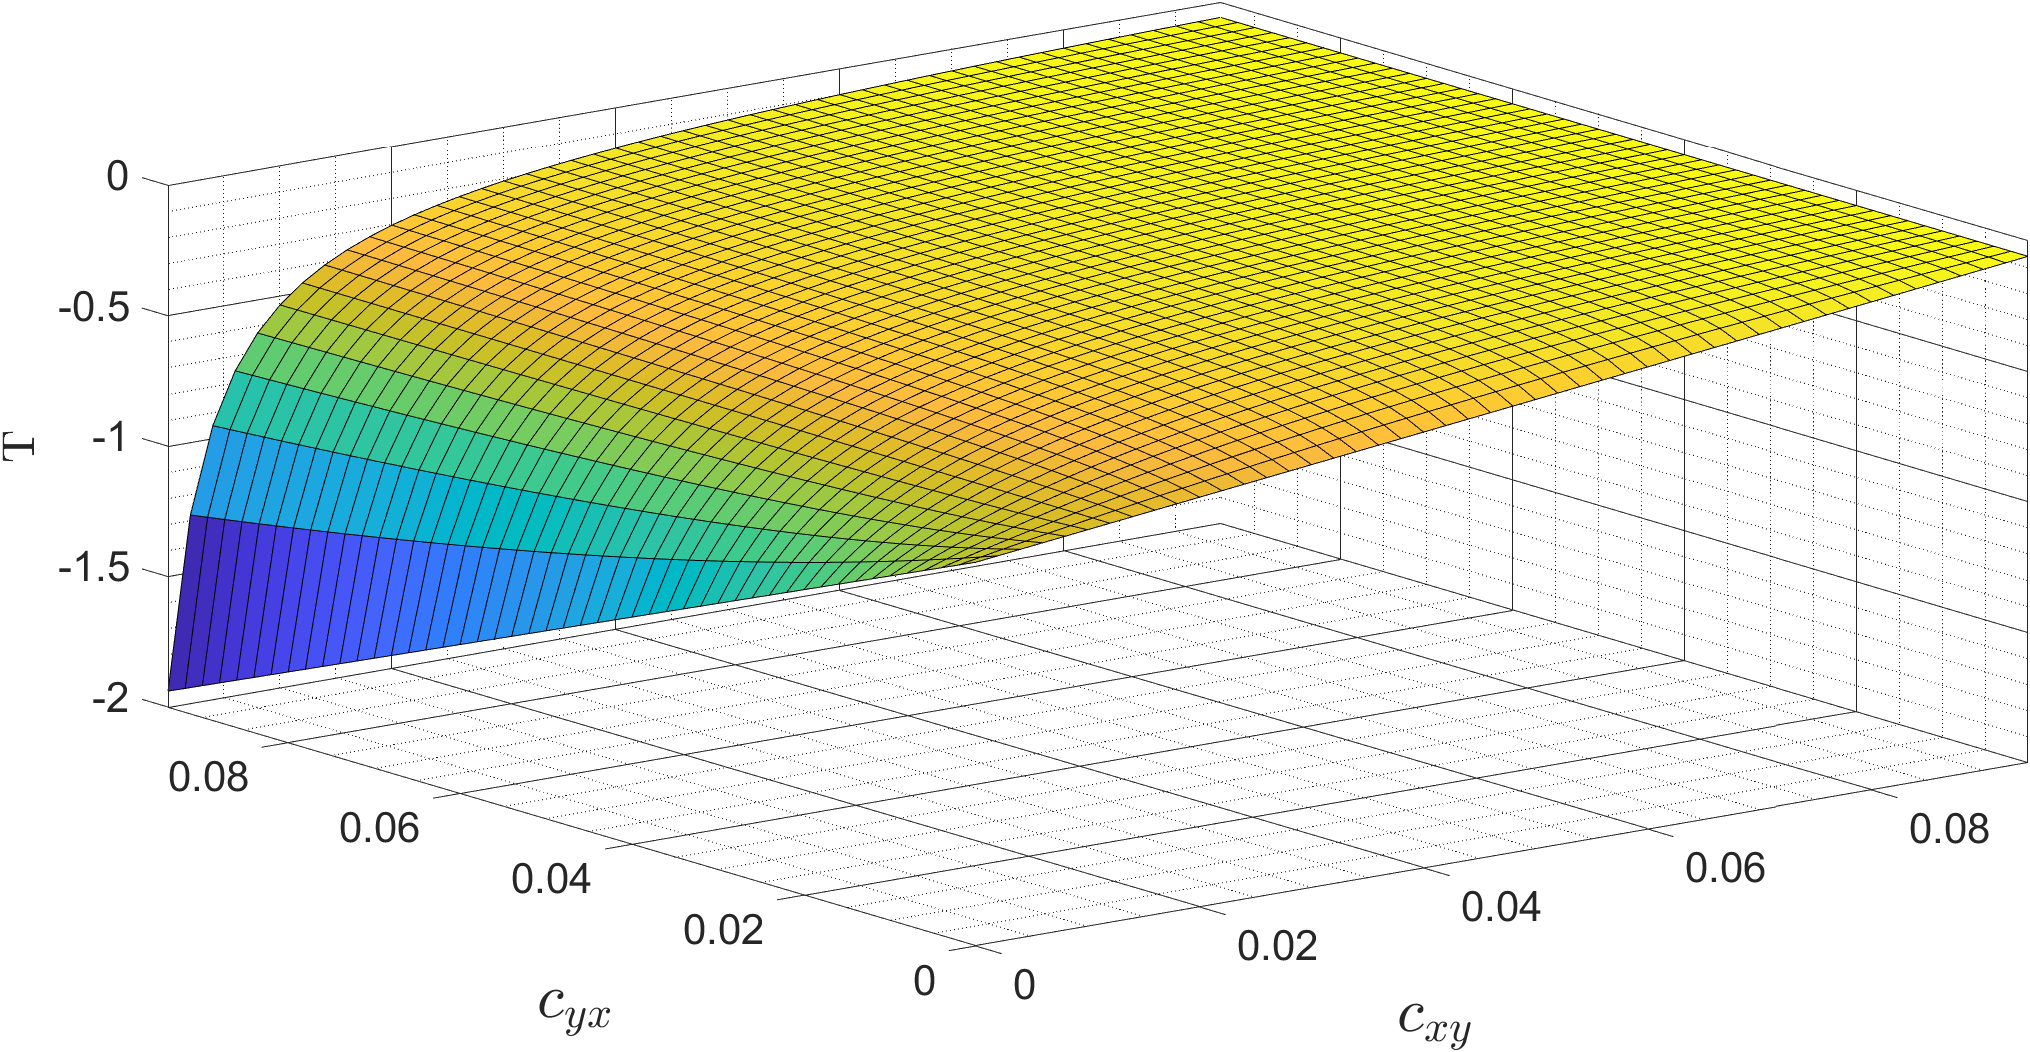
\includegraphics[width=14cm]{Pictures/Stability/Trace.png}
\end{figure}
\begin{figure}[H]
    \centering
    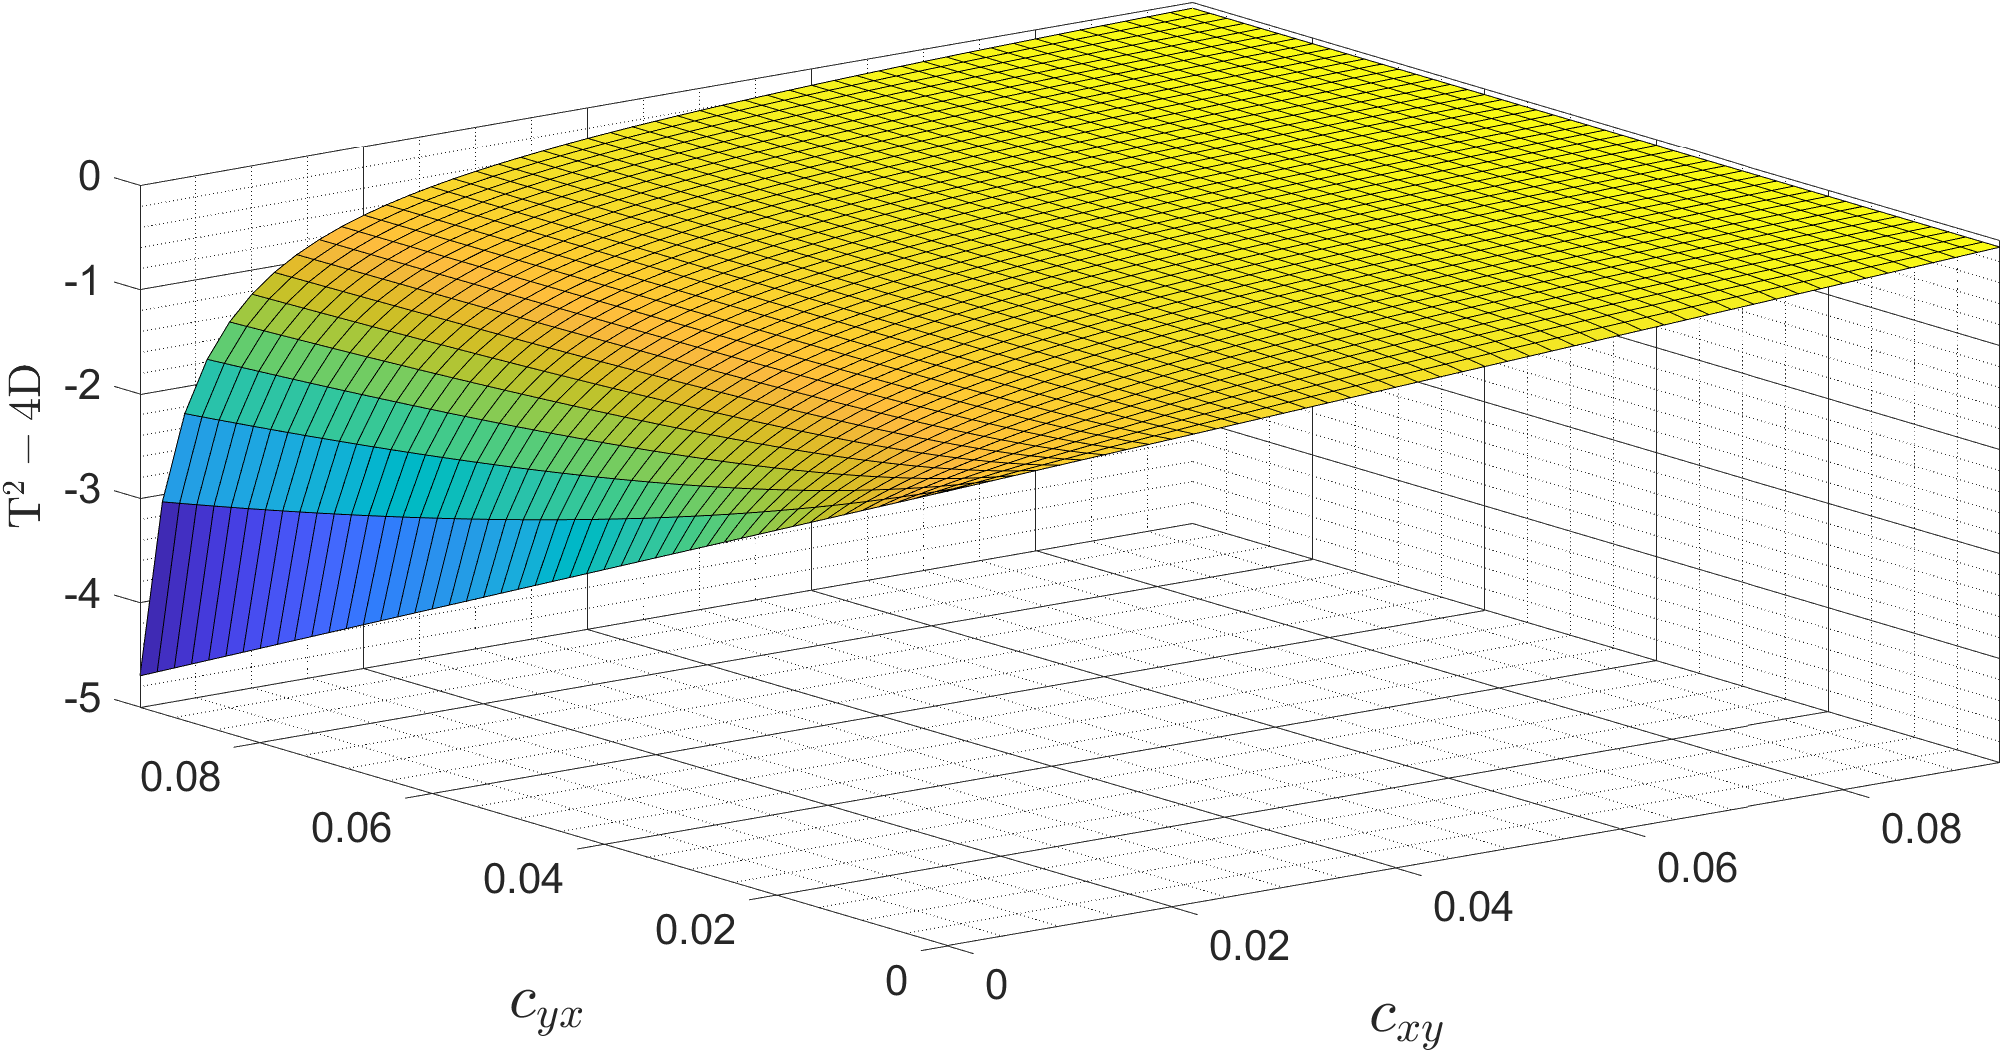
\includegraphics[width=14cm]{Pictures/Stability/Discriminant.png}
    \caption{\singlespacing
    The graphs above are the trace and discriminant of $\displaystyle J_{(x^*_4,y^*_4)}$ for different values of the parameters $c_{xy}$ and $c_{yx}$.}
    \label{fig:TraceDiscriminant}
\end{figure}
Notice that the trace and discriminant values are always negative for all $c_{xy}$ and $c_{yx}$ that belong in their constraints.
If we assume that $c_{yx}>c_{xy}$, then we are stating that the impact of salmon on brown bears is greater than brown bears on salmon.
However, brown bears eat a large quantity of salmon yearly, which means to support a brown bear's diet, there would need to be an abundance of salmon, whereas one brown bear kills thousands of salmon yearly ~\cite{deacy2018phenological,hilderbrand1999effect}.
So, the brown bear population should have a higher effect on the salmon population.
Therefore, the constraints for the parameters $c_{xy}$ and $c_{yx}$ are
\begin{equation*}
    \begin{array}{c}
         0<c_{xy}<0.094,  \\
         0<c_{yx}<c_{xy}.
    \end{array}
\end{equation*}
% The values for the discriminant, $\mathrm{T}^2-4\mathrm{D}$, and trace, $\mathrm{T}$, can be plotted by designing a meshgrid for the parameters $c_{xy}$ and $c_{yx}$ based on their constraints as shown below.

% \vspace{2.5cm}

% \begin{figure}[H]
%     \centering
%     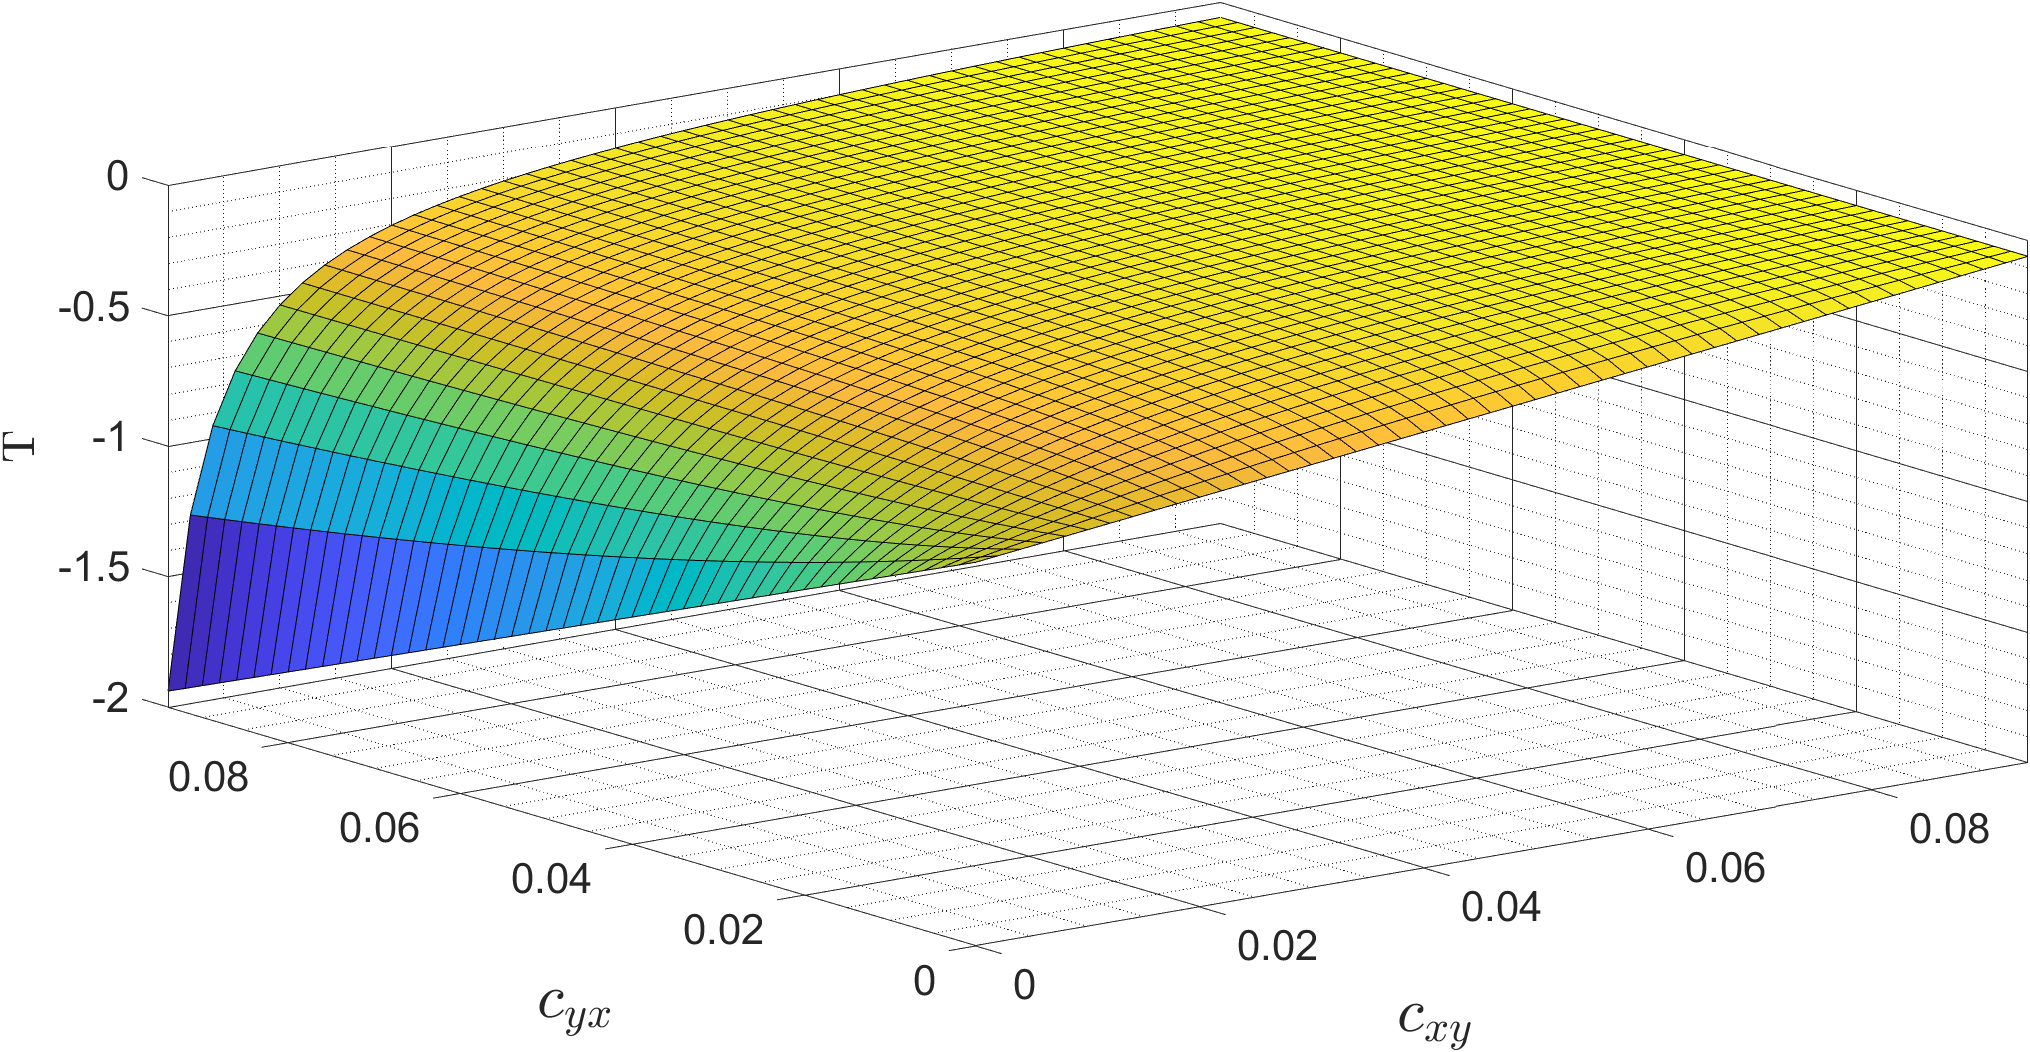
\includegraphics[width=14cm]{Pictures/Stability/Trace.png}
% \end{figure}
% \begin{figure}[H]
%     \centering
%     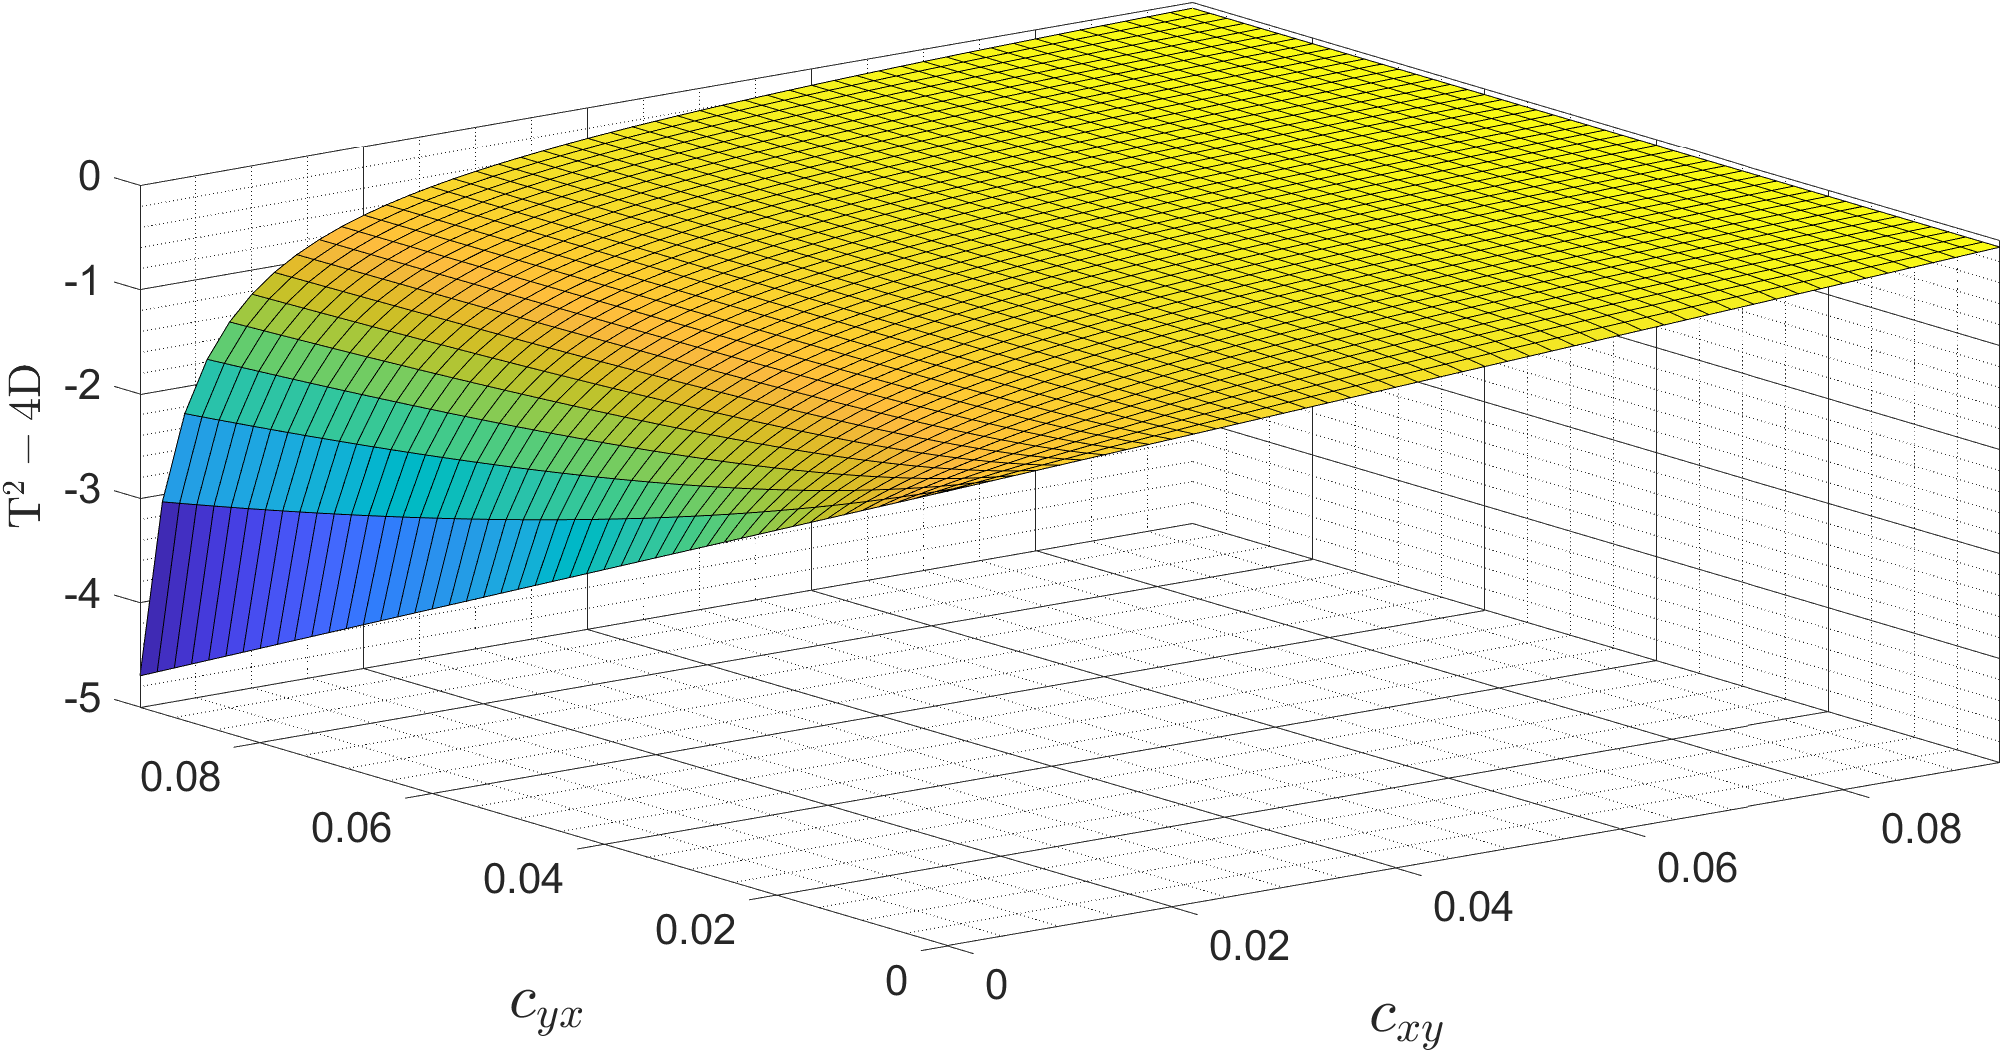
\includegraphics[width=14cm]{Pictures/Stability/Discriminant.png}
%     \caption{The graphs above are the trace and discriminant of $\displaystyle J_{(x^*_4,y^*_4)}$ for different values of the parameters $c_{xy}$ and $c_{yx}$.}
%     \label{fig:TraceDiscriminant}
% \end{figure}
% Notice that the trace and discriminant values are always negative for all $c_{xy}$ and $c_{yx}$ that belong in their constraints.
Looking at \figureautorefname~\ref{fig:TraceDiscriminant} from a top-down view, we can see which values for $c_{xy}$ and $c_{yx}$ satisfy the new constraints.

\vspace{3cm}

\begin{figure}[H]
    \centering
    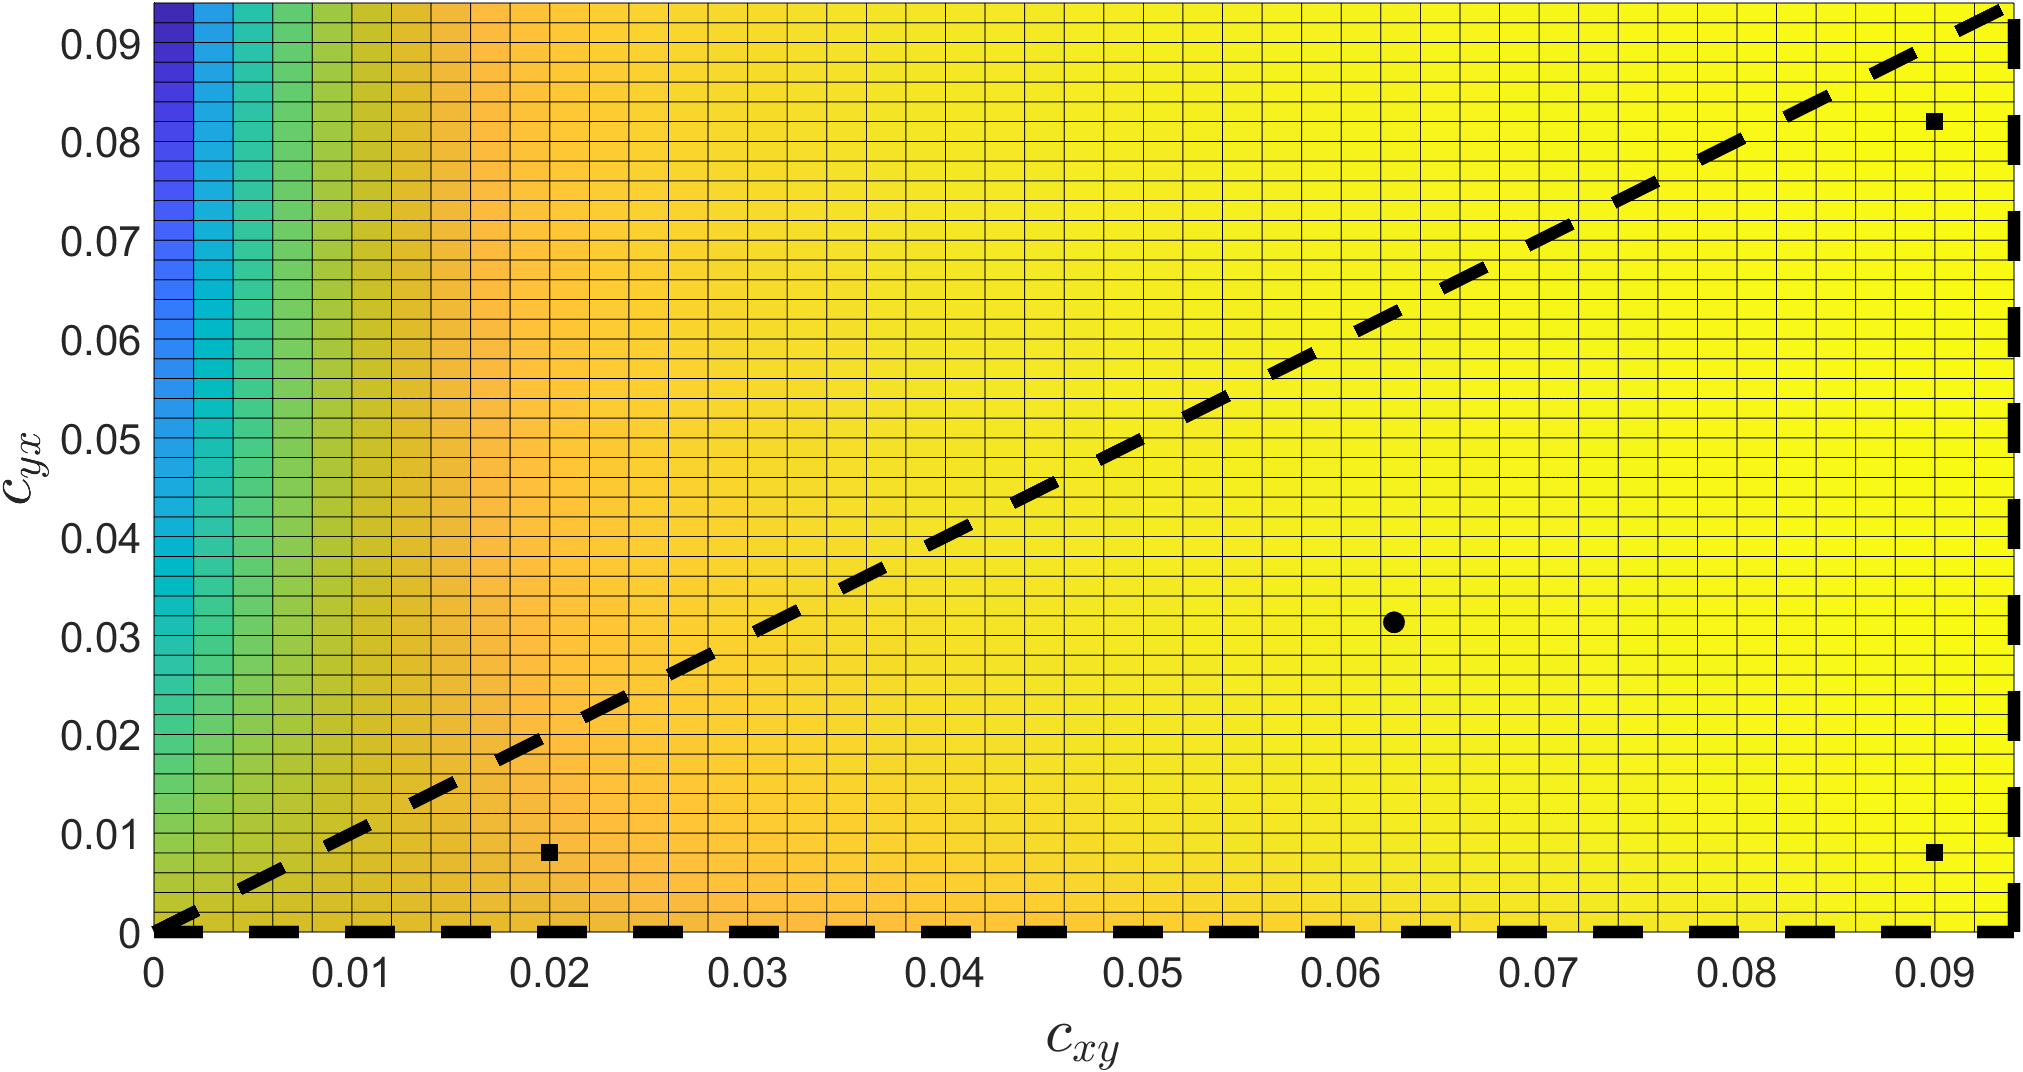
\includegraphics[width=14cm]{Pictures/Stability/TraceTopDown.png}
\end{figure}
\begin{figure}[H]
    \centering
    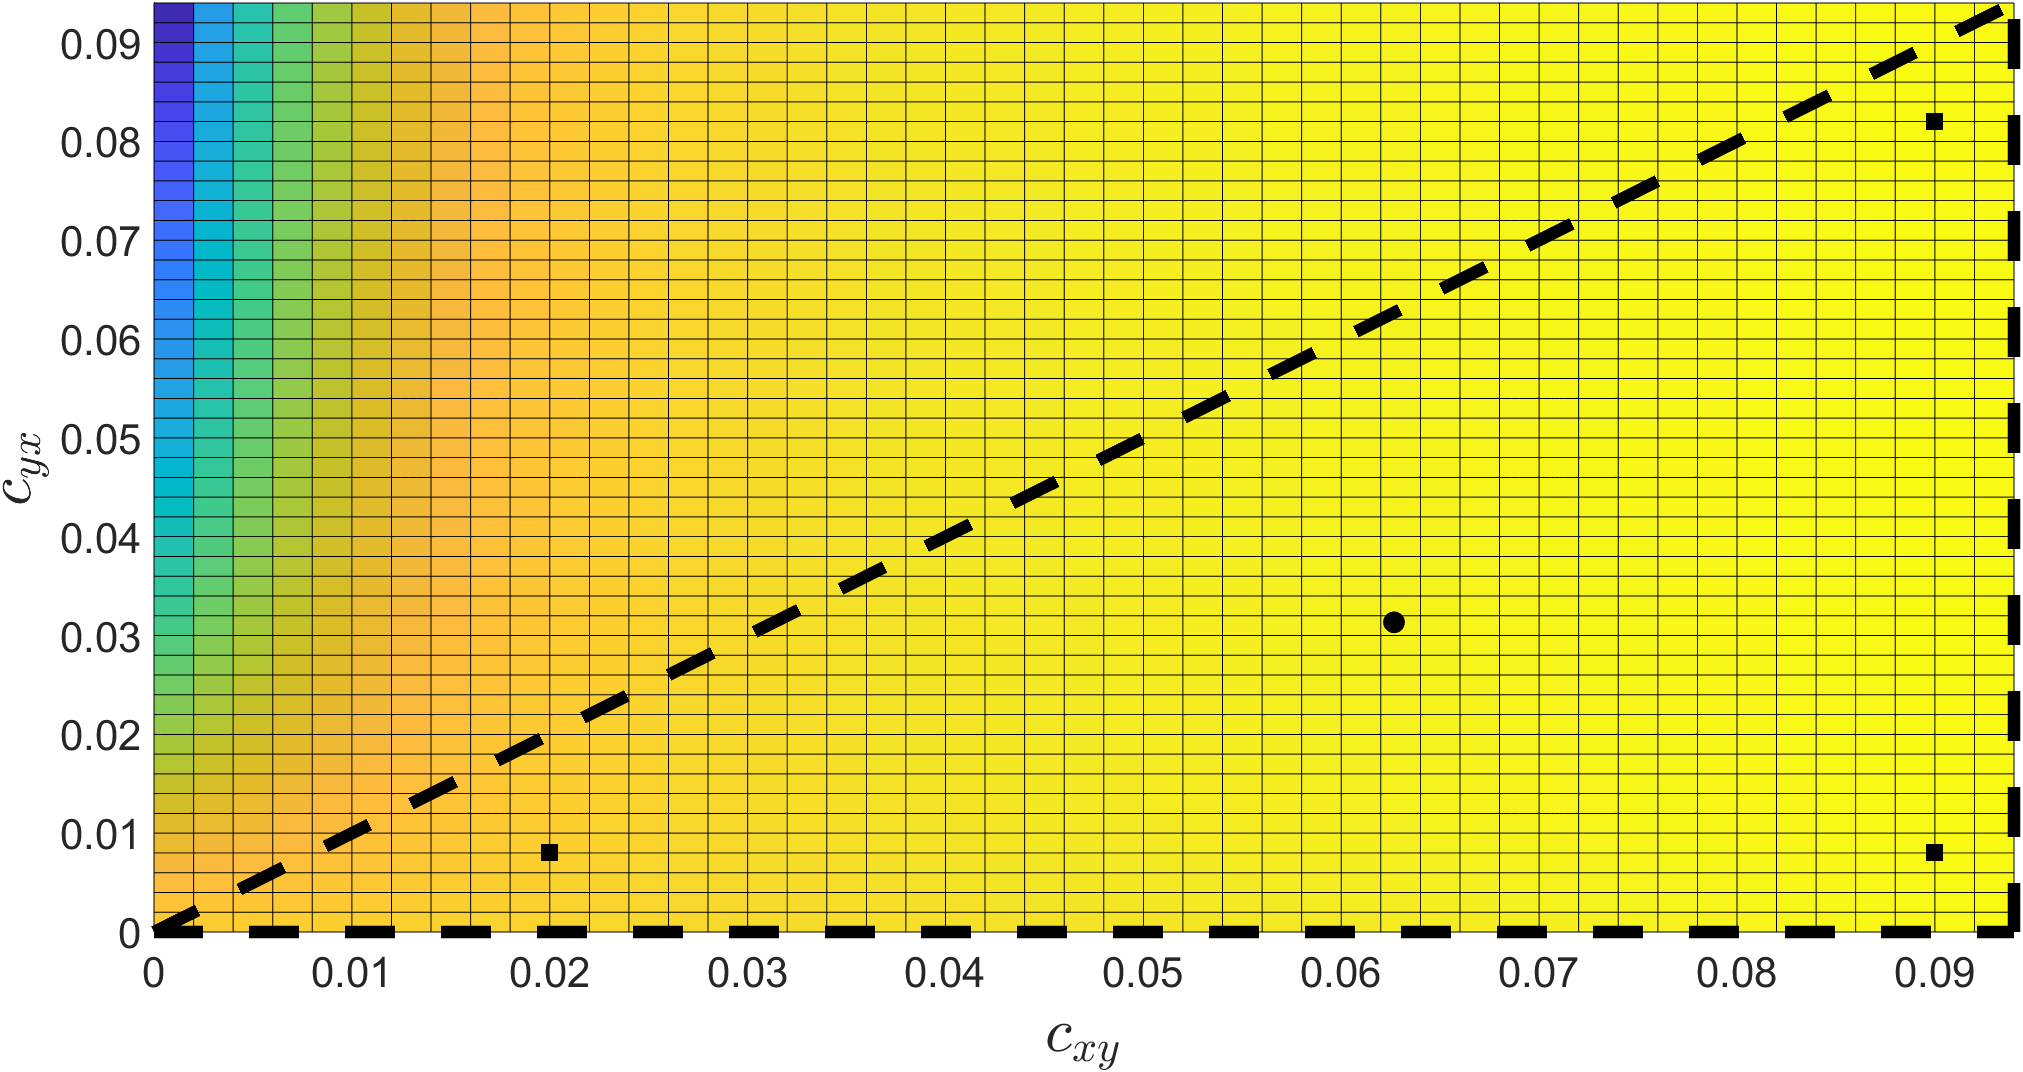
\includegraphics[width=14cm]{Pictures/Stability/DiscriminantTopDown.png}
    \caption{\singlespacing
    Top-down view of \figureautorefname~\ref{fig:TraceDiscriminant}. The points inside the right triangle are all values that satisfy the constraints of parameters $c_{xy}$ and $c_{yx}$. The right triangle's center of mass is marked with a black dot at the coordinate point $(0.0627,0.0313)$.}
    \label{fig:TraceDiscriminantTopDown}
\end{figure}
Now, we begin testing different $c_{xy}$ and $c_{yx}$ values to illustrate how different interaction rates affect the outcome of each species' population.
The values chosen for $(c_{xy},\;c_{yx})$ are $(0.02,\;0.008)$, $(0.09,\;0.008)$, $(0.09,\;0.082)$, and $(0.0627,\;0.0313)$. These pair of interaction parameters can be seen plotted in the figure above.
To compare each of the parameters, we plot the solutions to \equationautorefname~\eqref{eq:AutonomousSystemODEs}, where the brown bear population is along the y-axis, and the salmon population is along the x-axis as shown below for each pair of parameters.
\begin{figure}[H]
    \centering
    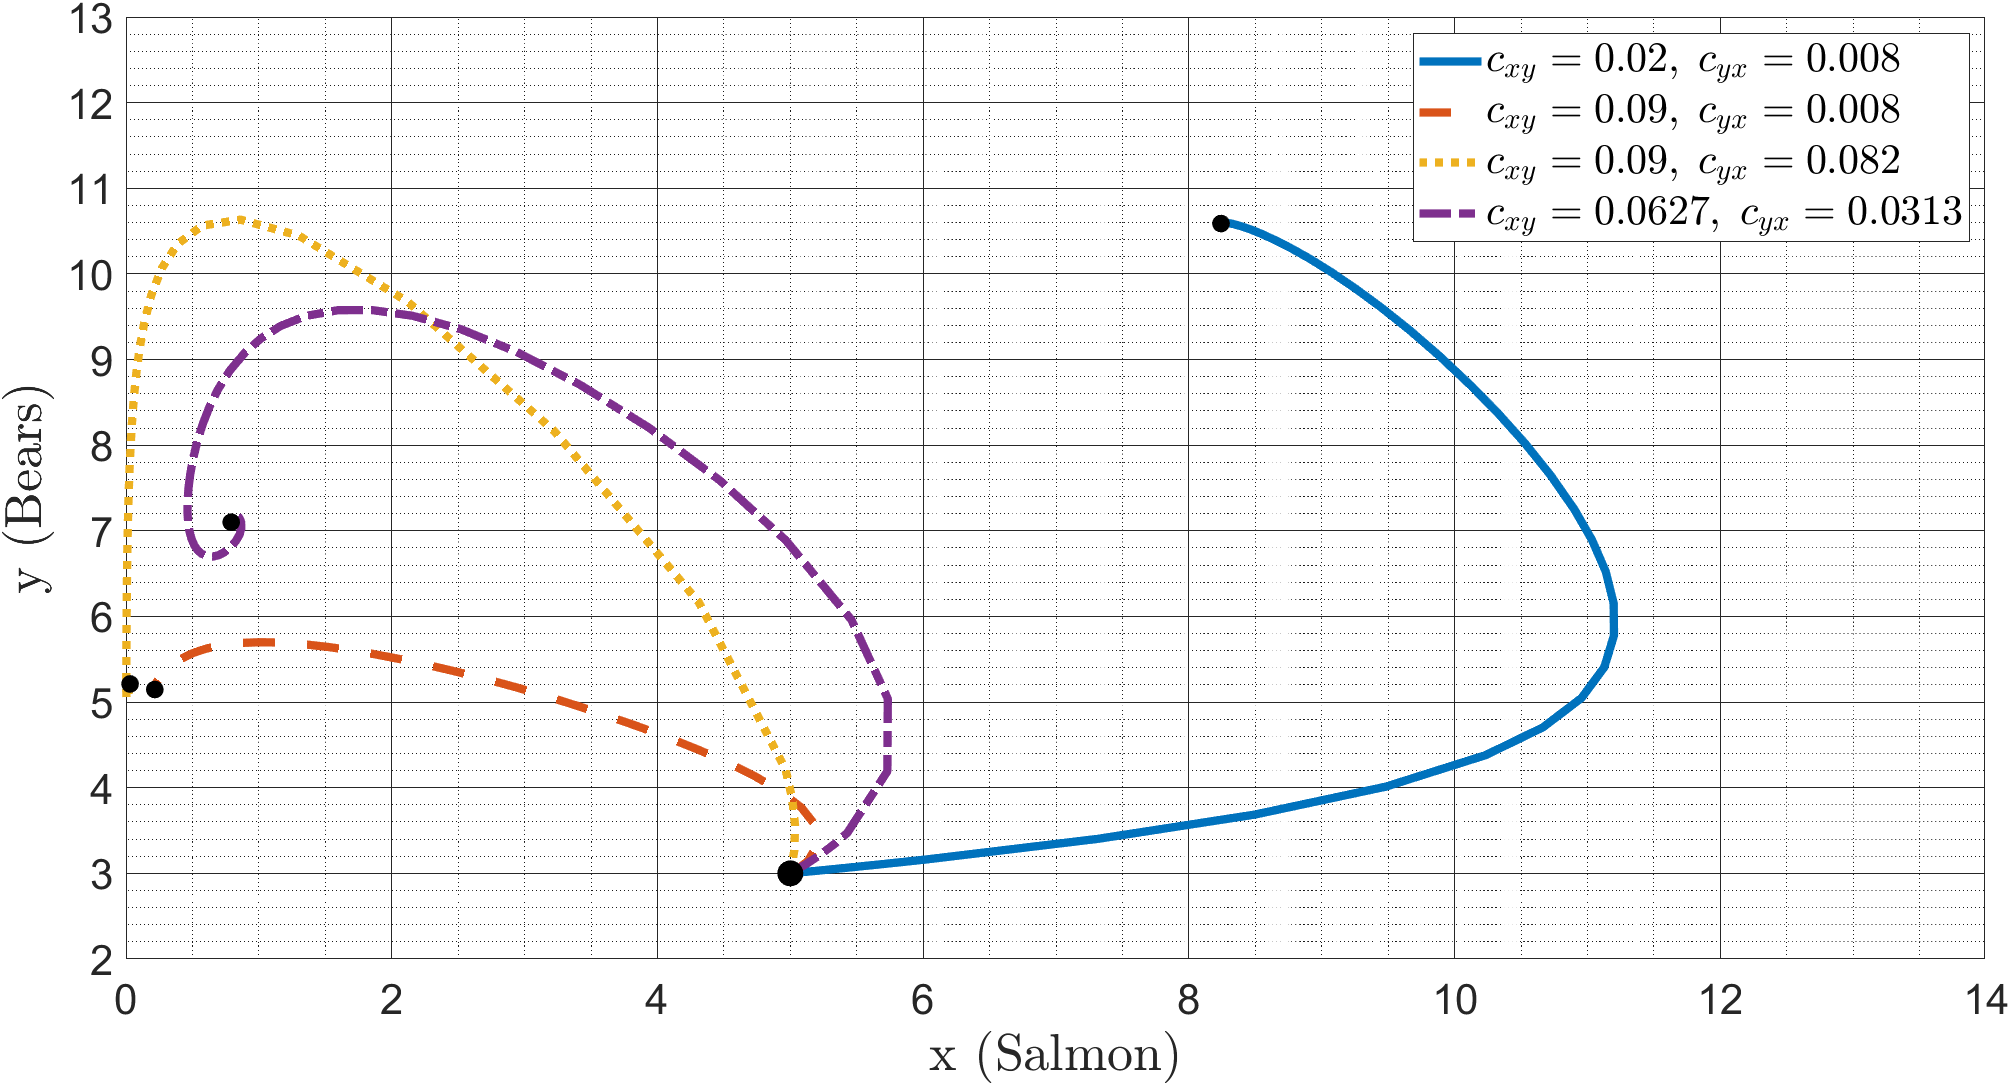
\includegraphics[width=14cm]{Pictures/Stability/SolutionsAutonomousModel.png}
    \caption{\singlespacing
    Compares the effect of different interaction rates, $(c_{xy},\;c_{yx})$, for the autonomous model, \equationautorefname~\eqref{eq:AutonomousSystemODEs}, where the initial conditions are $x_0 = 5$ and $y_0 = 3$.}
    \label{fig:SolutionsAutonomous}
\end{figure}
The graph above shows that each of these parameters affects the location of the critical point, $(x^*_4,y^*_4)$, as well as the oscillations of the populations.
We chose the initial conditions, $x_0 = 5$ and $y_0 = 3$, to illustrate the dramatic difference in interaction parameters.
When $c_{xy}$ is large, the salmon population dies off, and when $c_{yx}$ is large, the brown bear population increases faster before converging near its carrying capacity.
Lastly, when the pair of parameters is equal to the right triangle's center of mass in \figureautorefname~\ref{fig:TraceDiscriminantTopDown}, the population oscillates and converges to its critical point $(0.79,7.1)$.
We use $c_{xy}=0.0627$ and $c_{yx}=0.0313$ to represent the interaction rates of the two species for \equationautorefname~\eqref{eq:AutonomousSystemODEs} because with these parameters, the populations oscillate around their critical point much longer than the other parameters we tested, which will provide a more visible comparison for when we incorporate climate change.
So, with all the parameters selected, the solutions to the autonomous model, \equationautorefname~\eqref{eq:AutonomousSystemODEs}, with respect to time, are shown below.
\begin{figure}[H]
    \centering
    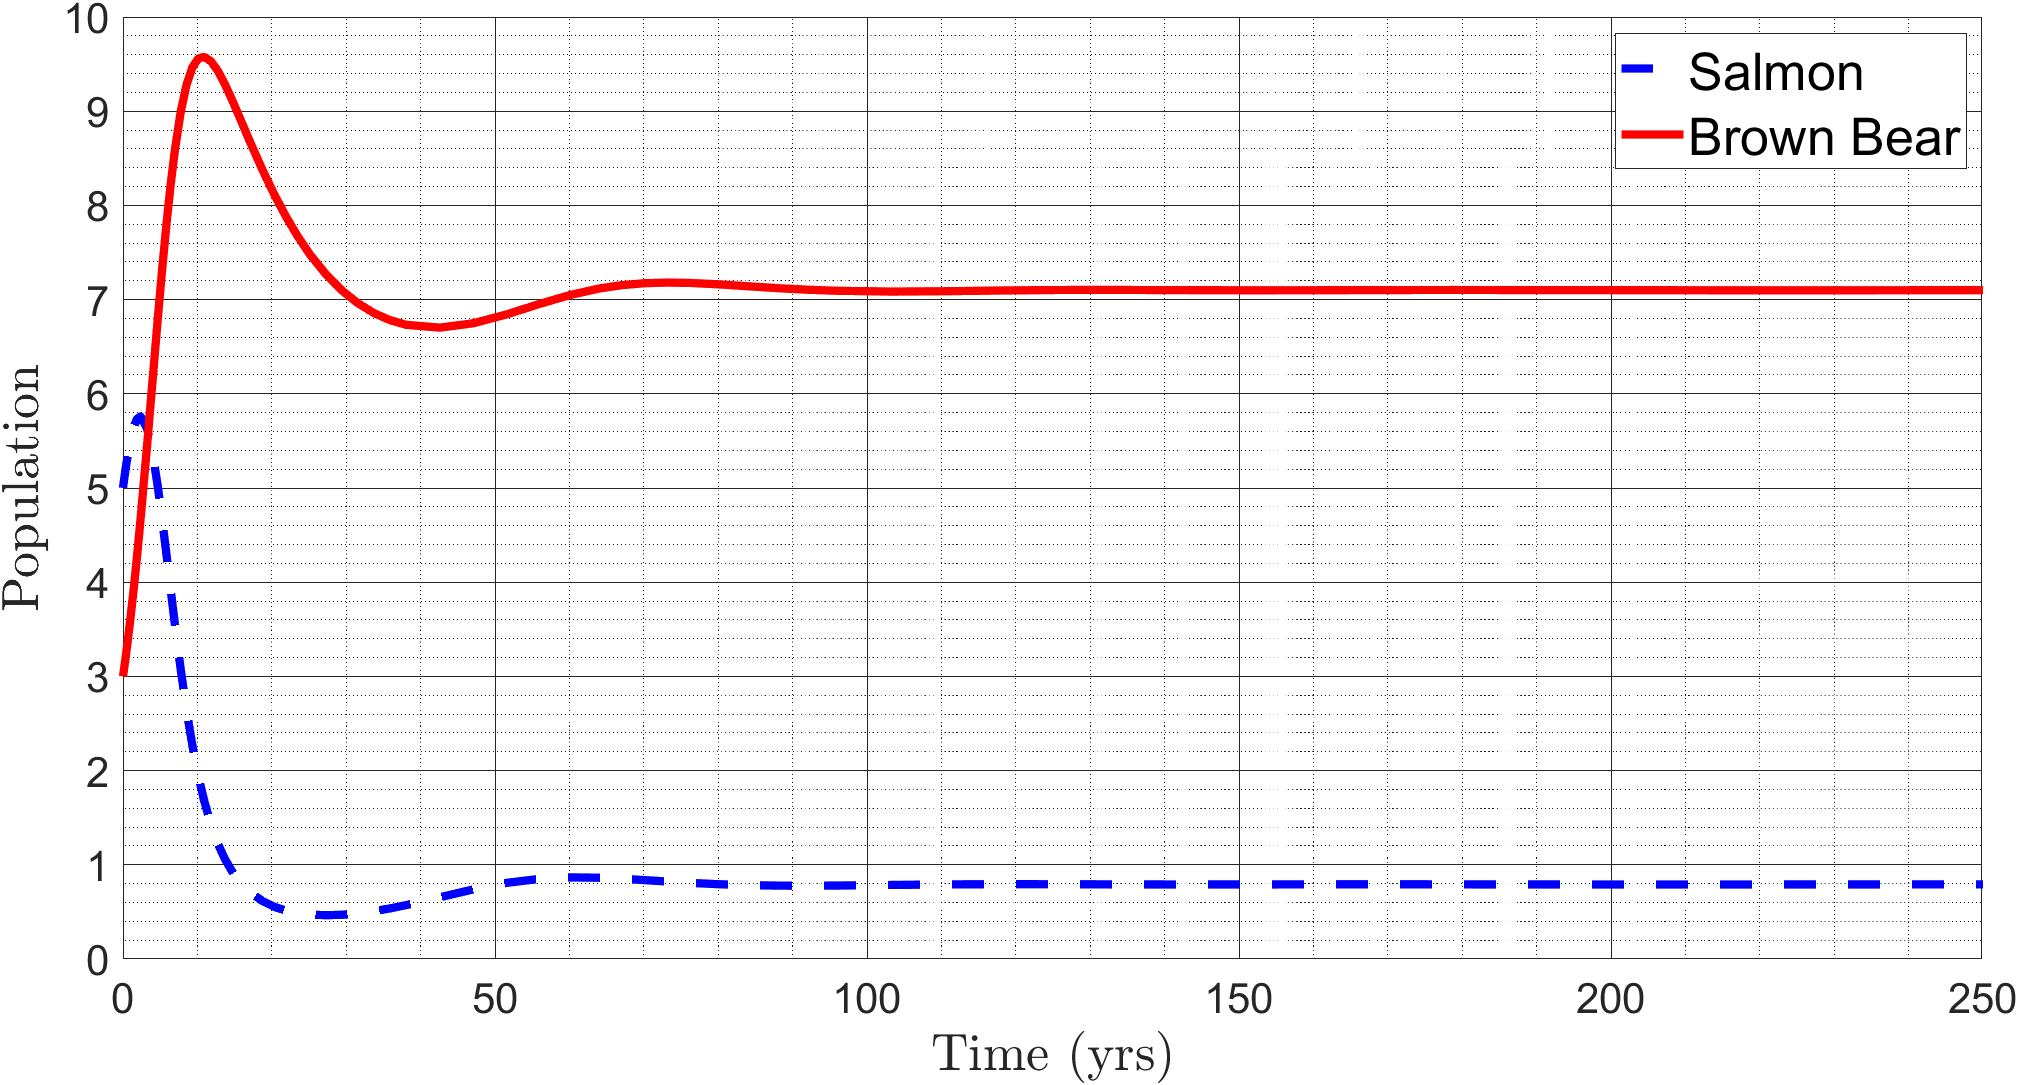
\includegraphics[width=14cm]{Pictures/System ODEs/AutonomousModelRespectTime.png}
    \caption{\singlespacing
    Plot of  the solutions to the autonomous model, \equationautorefname~\eqref{eq:AutonomousSystemODEs}, with respect to time.}
    \label{fig:SolutionsNonAutonomous}
\end{figure}
In the figure above, both populations briefly increase before changing directions and oscillating toward their equilibrium points.
Based on this figure, the brown bear population quickly overtook the salmon population, forcing the salmon near regional extinction.


% \section{Picking Interaction Parameters}

% % % First, we look at the effects of $c_{xy}$ and $c_{yx}$ on the critical points of \equationautorefname~\eqref{eq:AutonomousSystemODEs}.
% Before, finding the critical points of the system of ODEs, we fix the parameter, $T$, to the optimal temperature, $12.5^{\circ}$C, to eliminate the effect of temperature on the salmon population.
% Now, the equations can be rewritten as:
% \begin{equation}
%     \begin{aligned}
%     \frac{dx}{dt} &= R(T_{opt})x -\frac{R(T_{opt})x^2}{K_x} - c_{xy}xy,\\[.4cm]
%     \frac{dy}{dt} &=r_yy -\frac{r_yy^2}{K_y} + c_{yx}xy.
%     \end{aligned}
% \end{equation}
% Then, substituting $ a_x = R(T_{opt})$, $\displaystyle b_x = \frac{R(T_{opt})}{K_x}$, $a_y = r_y$, and $\displaystyle b_y = \frac{r_y}{K_y}$ a similar model to Theodore Modis' model, \equationautorefname~\eqref{eq:modislotkavoltera}, is constructed.
% Before beginning the analysis of \equationautorefname~\eqref{eq:AutonomousSystemODEs}, values must be assigned to $c_{xy}$ and $c_{yx}$.
% First, we will develop a criteria for these parameters such that the solutions will reflect their behavior.
% We know that the model should be stable near its critical points because if they were unstable, the populations could approach infinity.
% Second, the populations of the species should be oscillating as can be seen in \tablename~\ref{tab:runvsweight}.
% To achieve a stable oscillation at a critical point, we will evaluate the solutions to the model when the eigenvalues for the critical point have non-positive real parts and imaginary parts.

% Since \equationautorefname~\eqref{eq:AutonomousSystemODEs} is non-autonomous, then we can't evaluate it's fixed points.
% So, replacing the salmon model with \equationautorefname~\eqref{eq:salmonlogisticrepo}, and fixing $T=T_{opt}$, produces the below autonomous model.
% \begin{equation}\label{eq:THENonModel}
%     \begin{aligned}
%     \frac{dx}{dt} &= \ln{(R(T_{opt}))}x\left(1-\frac{x}{K_x}\right) - c_{xy}xy,\\[.4cm]
%     \frac{dy}{dt} &=ry\left(1-\frac{y}{K_y}\right) + c_{yx}xy.
%     \end{aligned}
% \end{equation}
% Fixing $T$ to the constant, $T_{opt}$, eliminates the effect of temperature on the salmon population.
% Applying the distributive property to the above system of equations generates the following equations.
% \begin{equation*}
%     \begin{aligned}
%     \frac{dx}{dt} &= \ln{(R(T_{opt}))}x -\frac{\ln{(R(T_{opt}))}x^2}{K_x} - c_{xy}xy,\\[.4cm]
%     \frac{dy}{dt} &=r_yy -\frac{r_yy^2}{K_y} + c_{yx}xy.
%     \end{aligned}
% \end{equation*}
% Then, substituting $ a_x = \ln(R(T_{opt}))$, $\displaystyle b_x = \frac{\ln(R(T_{opt}))}{K_x}$, $a_y = r_y$, and $\displaystyle b_y = \frac{r_y}{K_y}$ a similar model to Theodore Modis' model, \equationautorefname~\eqref{eq:modislotkavoltera}, is constructed.
% \begin{equation}\label{eq:AutonomousSystemODEsModis}
%     \begin{aligned}
%     \frac{dx}{dt} &= a_xx - b_xx^2 - c_{xy}xy,\\
%     \frac{dy}{dt} &= a_yy - b_yy^2 + c_{yx}xy.
%     \end{aligned}
% \end{equation}
% Now, we set the above system of equations equal to the $\Vec{0}$.
% \begin{equation*}
%     \begin{aligned}
%     0 &= x(a_x - b_xx - c_{xy}y),\\
%     0 &= y(a_y - b_yy + c_{yx}x).
%     \end{aligned}
% \end{equation*}
% Then, solving for $x$ and $y$ produces the critical points below.
% \begin{equation*}
%     \begin{array}{ll}
%          x^*_1 = 0, & y^*_1 = 0,  \\
%          x^*_2 = K_x, & y^*_2 = 0,\\
%          x^*_3 = 0, & y^*_3 = K_y,
%     \end{array}
% \end{equation*}
% \begin{equation*}\scalebox{1.2}{$
%     \begin{array}{ll}
%         x^*_4 = \frac{a_xb_y-c_{xy}a_y}{c_{xy}c_{yx}+b_xb_y} & y^*_4 = \frac{a_xc_{yx}+b_xa_y}{c_{xy}c_{yx}+b_xb_y}.
%     \end{array}$}
% \end{equation*}
The first three critical points do not contain either of our unknown parameters, $c_{xy},\;c_{yx}$, but the fourth critical value does.
% Note, neither population can be negative and $c_{xy},\;c_{yx}>0$, which creates the below criteria for these parameters.
% \begin{equation*}\scalebox{1.2}{$
% \begin{array}{c}
%      0<c_{xy} \leq \frac{a_xb_y}{a_y}, \\[.1cm]
%      c_{yx} \geq -\frac{b_xa_y}{a_x}.
% \end{array}$}
% \end{equation*}
% Since $a_x,\;b_x,\;a_y>0$, then the criteria above changes to:
% \begin{equation*}\scalebox{1.2}{$
% \begin{array}{c}
%      0<c_{xy} \leq \frac{a_xb_y}{a_y}, \\[.1cm]
%      c_{yx} > 0.
% \end{array}$}
% \end{equation*}
% If we assume that $c_{yx}>c_{xy}$, this would imply that the rate at which salmon affect brown bears is higher than the rate at which brown bears affect salmon. 
% However, brown bears eat a large quantity of salmon, but salmon do not have this direct impact on bears.
% So, the brown bear population should have a higher affect on the salmon population.
% Therefore, the constraint for the parameters $c_{xy}$ and $c_{yx}$ is as follows.
% \begin{equation*}
%     \begin{array}{c}
%          0<c_{xy}\leq \frac{a_xb_y}{a_y} = 0.104,  \\
%          0<c_{yx}<c_{xy}.
%     \end{array}
% \end{equation*}
% Now, assessing the eigenvalues of \equationautorefname~\eqref{eq:AutonomousSystemODEsModis} with the above constraint, will determine the stability around the critical point $(x^*_4,\;y^*_4)$~\cite{roussel2019stability}.
% The eigenvalues can be found by solving for the characteristic polynomial of the Jacobian matrix for \equationautorefname~\eqref{eq:AutonomousSystemODEsModis}~\cite{roussel2019stability}.
% \begin{equation}\label{eq:Jacobian}
%     J_{(x,y)} =
%     \begin{pmatrix}
%         a_x - 2b_xx -c_{xy}y & -c_{xy}x\\
%         c_{yx}y & a_y - 2b_yy + c_{yx}x
%     \end{pmatrix}.
% \end{equation}
% The characteristic polynomial of the above Jacobian matrix is displayed below.
% \begin{align}
% \begin{split}\label{eq:CharacteristicEq}\displaystyle
%     \text{det}(J_{(x,y)}-\lambda I) = \lambda^2 - \pmb{\big[}\; (a_x - 2b_xx -c_{xy}y) + (a_y - 2b_yy + c_{yx})\;\pmb{\big]}\lambda\\
%     + \pmb{\big[}\; (a_x - 2b_xx -c_{xy}y)(a_y - 2b_yy + c_{yx}) + c_{xy}xc_{yx}y\;\pmb{\big]}.
% \end{split}
% \end{align}
% Note that:
% \begin{equation*}
%     \begin{array}{ll}
%          \mathrm{T} &= \text{tr}(J_{(x,y)}) = (a_x - 2b_xx -c_{xy}y) + (a_y - 2b_yy + c_{yx}),
%          \\
%          \mathrm{D} &= \text{det}(J_{(x,y)}) = (a_x - 2b_xx -c_{xy}y)(a_y - 2b_yy + c_{yx}) + c_{xy}xc_{yx}y.
%     \end{array}
% \end{equation*}
% So, substituting in the above variables in \equationautorefname~\eqref{eq:CharacteristicEq} produces:
% \begin{equation*}
%     \text{det}(J_{(x,y)}-\lambda I) = \lambda^2 - \mathrm{T}\lambda + \mathrm{D}.
% \end{equation*}
% Now, setting the above equation equal to zero and solving for our eigenvalues, $\lambda$, gives the below equation.
% \begin{equation*}
%     \lambda = \frac{\mathrm{T} \pm \sqrt{\mathrm{T}^2 - 4\mathrm{D}}}{2}.
% \end{equation*}
% As mentioned earlier, the stability for $(x^*_4,\;y^*_4)$ can be found by analyzing the eigenvalues.
% To achieve a stable oscillation the eigenvalues for the critical point have to contain non-positive real parts and imaginary parts~\cite{roussel2019stability}.
% This implies that $\displaystyle \mathrm{T} \leq 0$ and $\displaystyle \mathrm{T}^2 - 4\mathrm{D} < 0$.
% So for the critical point, $(x^*_4,\;y^*_4)$:
% \begin{equation*}\scalebox{1.2}{$
%     \begin{array}{cc}
%         \mathrm{T} &=  \frac{a_y b_x (c_{xy}-b_y)-a_x b_y (b_x+c_{yx})}{b_x b_y+c_{xy} c_{yx}},\\[.1cm]
%         \mathrm{D} &= \frac{(a_x c_{yx}+a_y b_x) (a_x b_y-a_y c_{xy})}{b_x b_y+c_{xy} c_{yx}}.
%     \end{array}$}
% \end{equation*}
% The values for the discriminant, $\mathrm{T}^2-4\mathrm{D}$, and trace, $\mathrm{T}$, can be plotted by designing a meshgrid for the parameters $c_{xy}$ and $c_{yx}$ based on their constraints as shown below.

% \vspace{2.5cm}

% \begin{figure}[H]
%     \centering
%     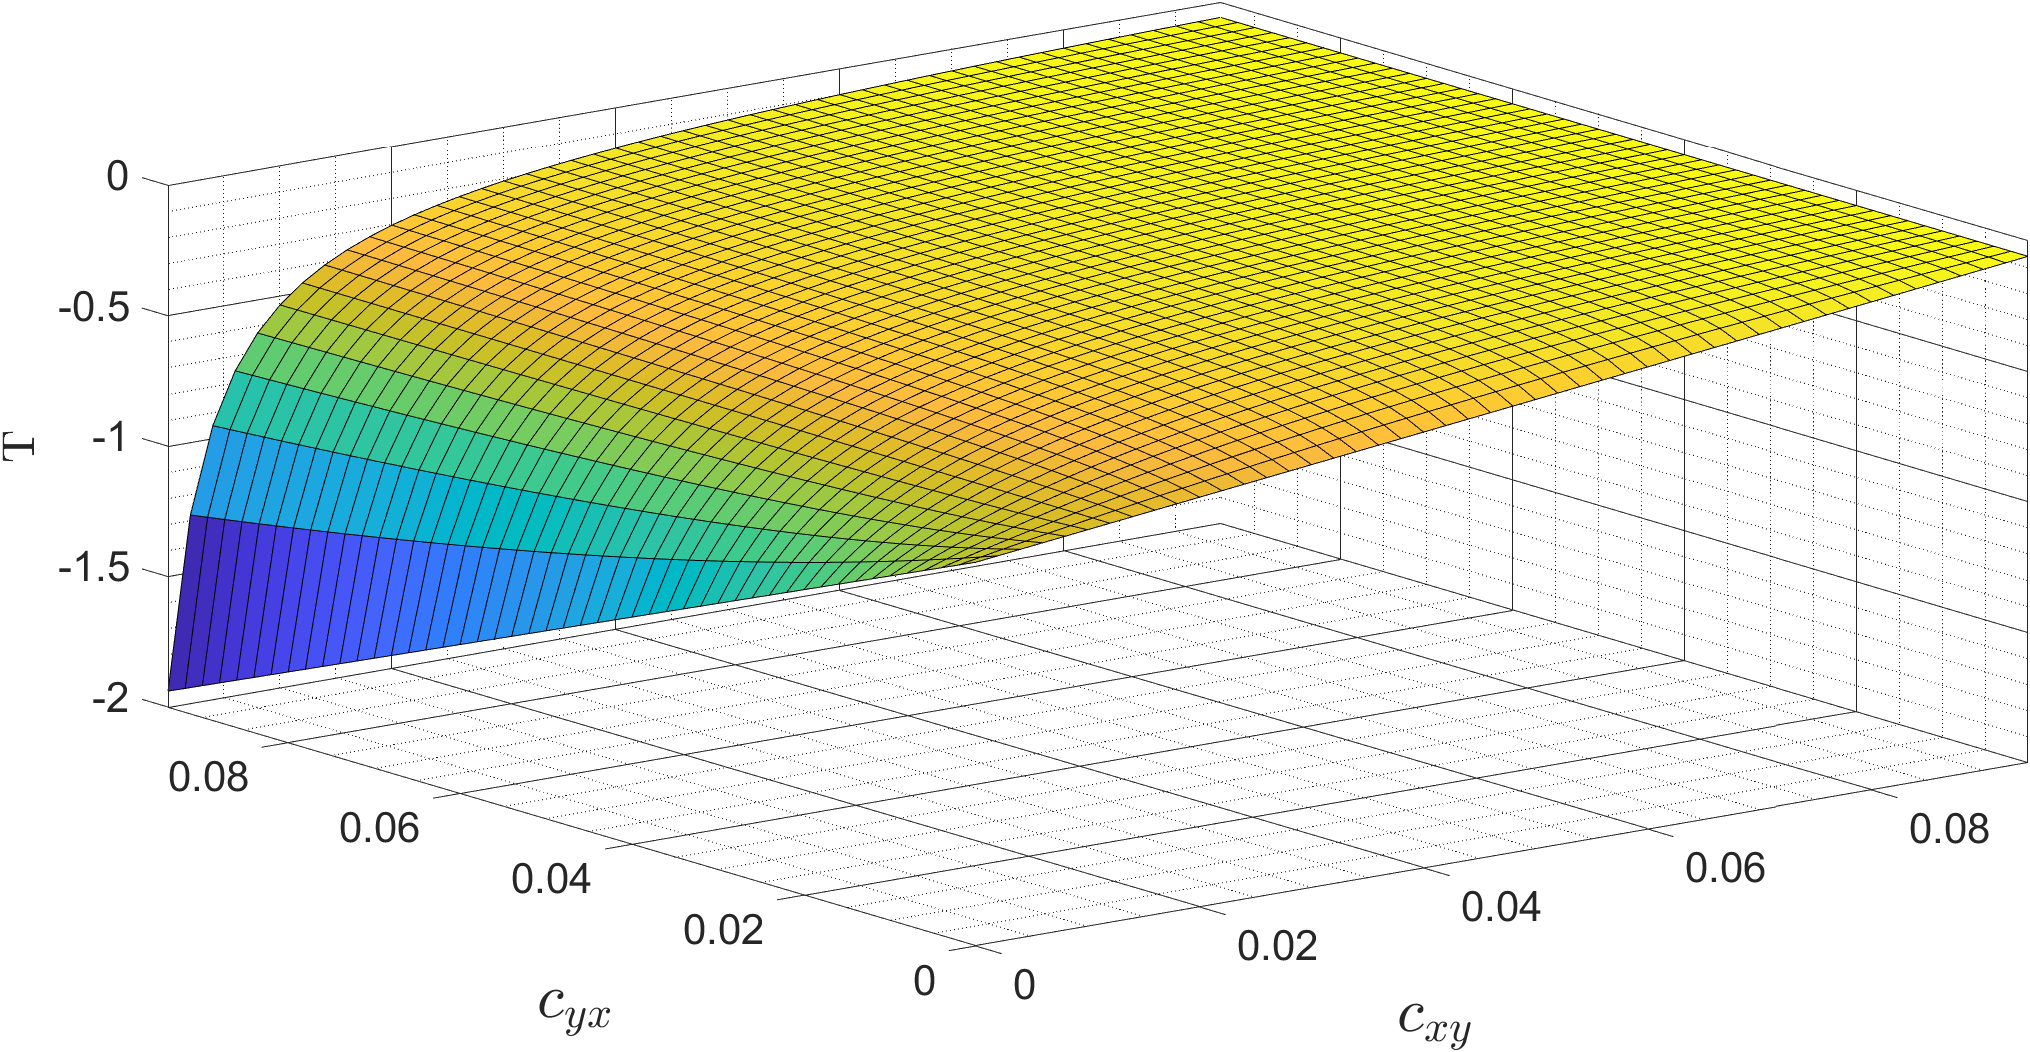
\includegraphics[width=14cm]{Pictures/Stability/Trace.png}
% \end{figure}
% \begin{figure}[H]
%     \centering
%     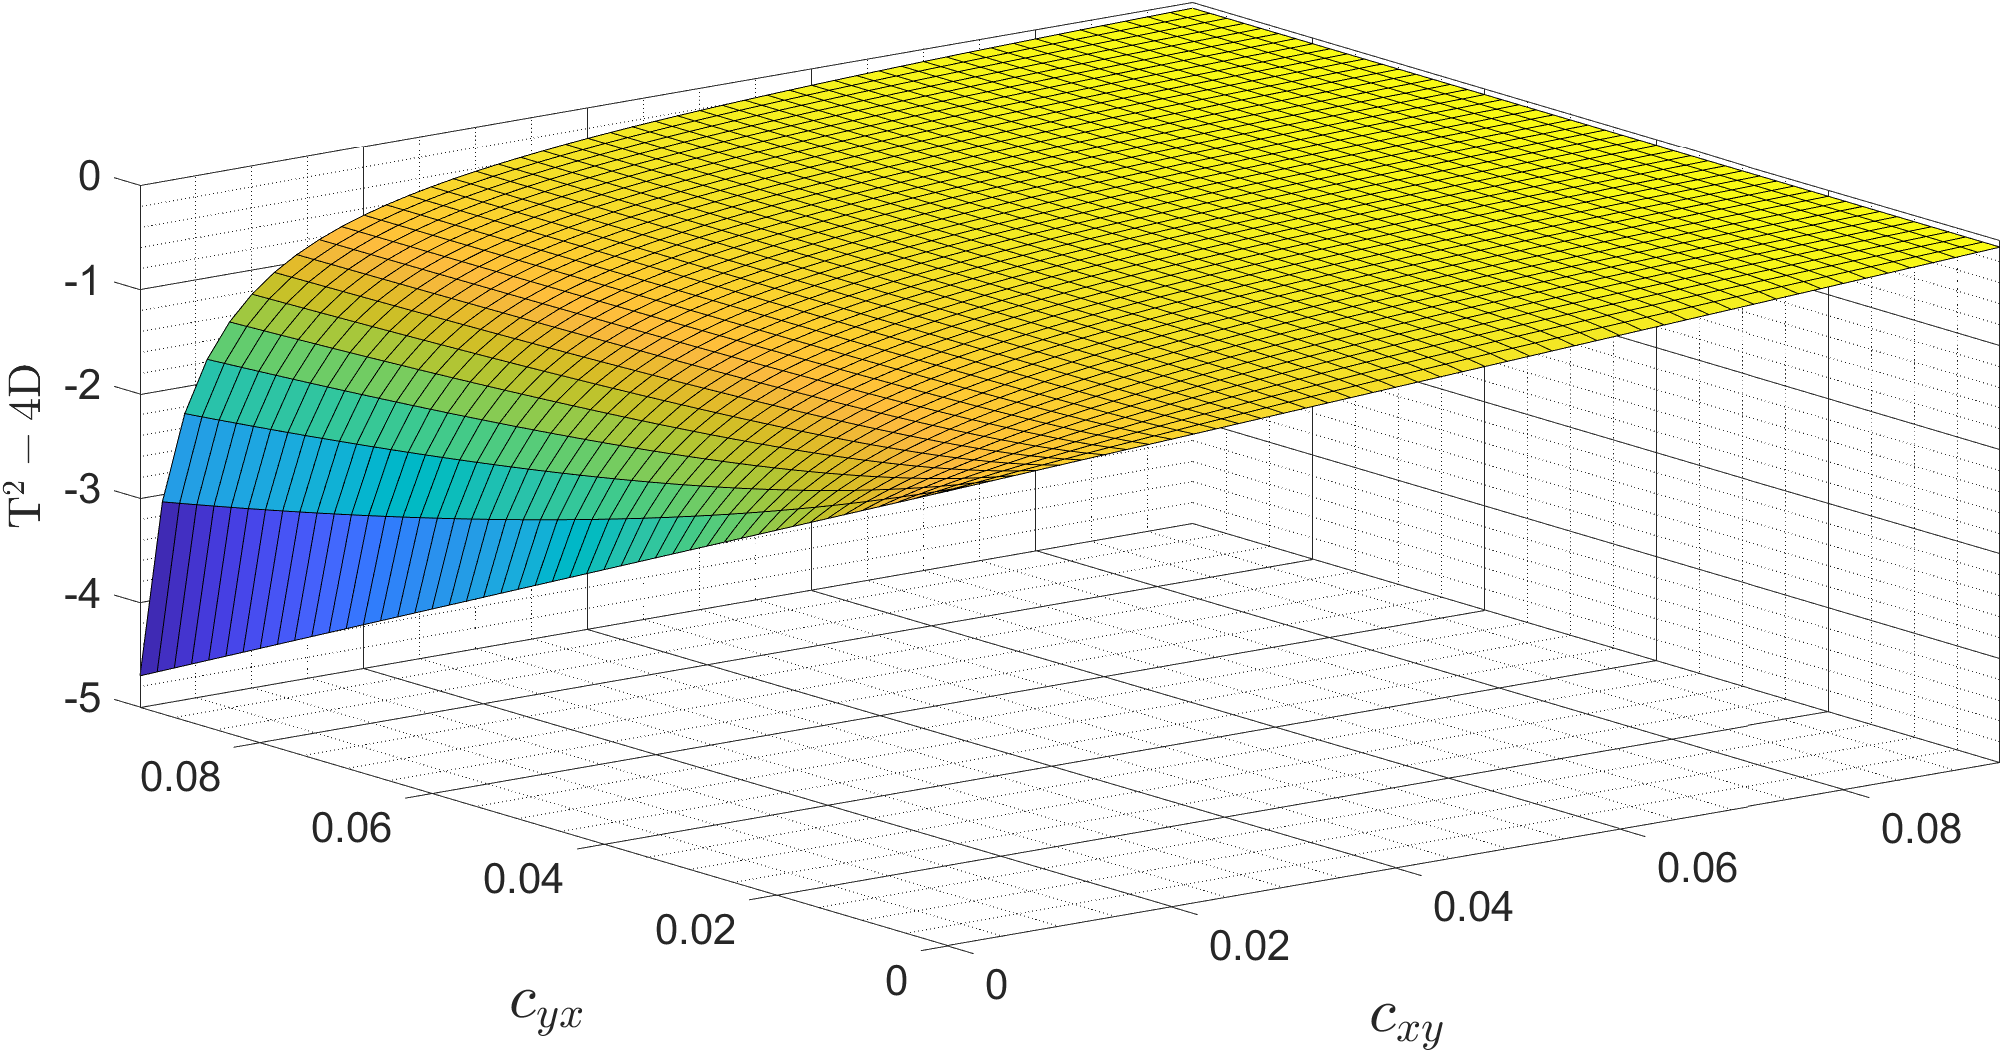
\includegraphics[width=14cm]{Pictures/Stability/Discriminant.png}
%     \caption{The graphs above are the trace and discriminant of $\displaystyle J_{(x^*_4,y^*_4)}$ for different values of the parameters $c_{yx}$ and $c_{xy}$.}
%     \label{fig:TraceDiscriminant}
% \end{figure}
% Notice that the values for the trace and discriminant are always negative for all $c_{yx}$ and $c_{xy}$ that belong in their constraints.
% Now, looking at these figure from a top-down view will provide a clear outline of which $c_{yx}$ and $c_{xy}$ values to test.
% \begin{figure}[H]
%     \centering
%     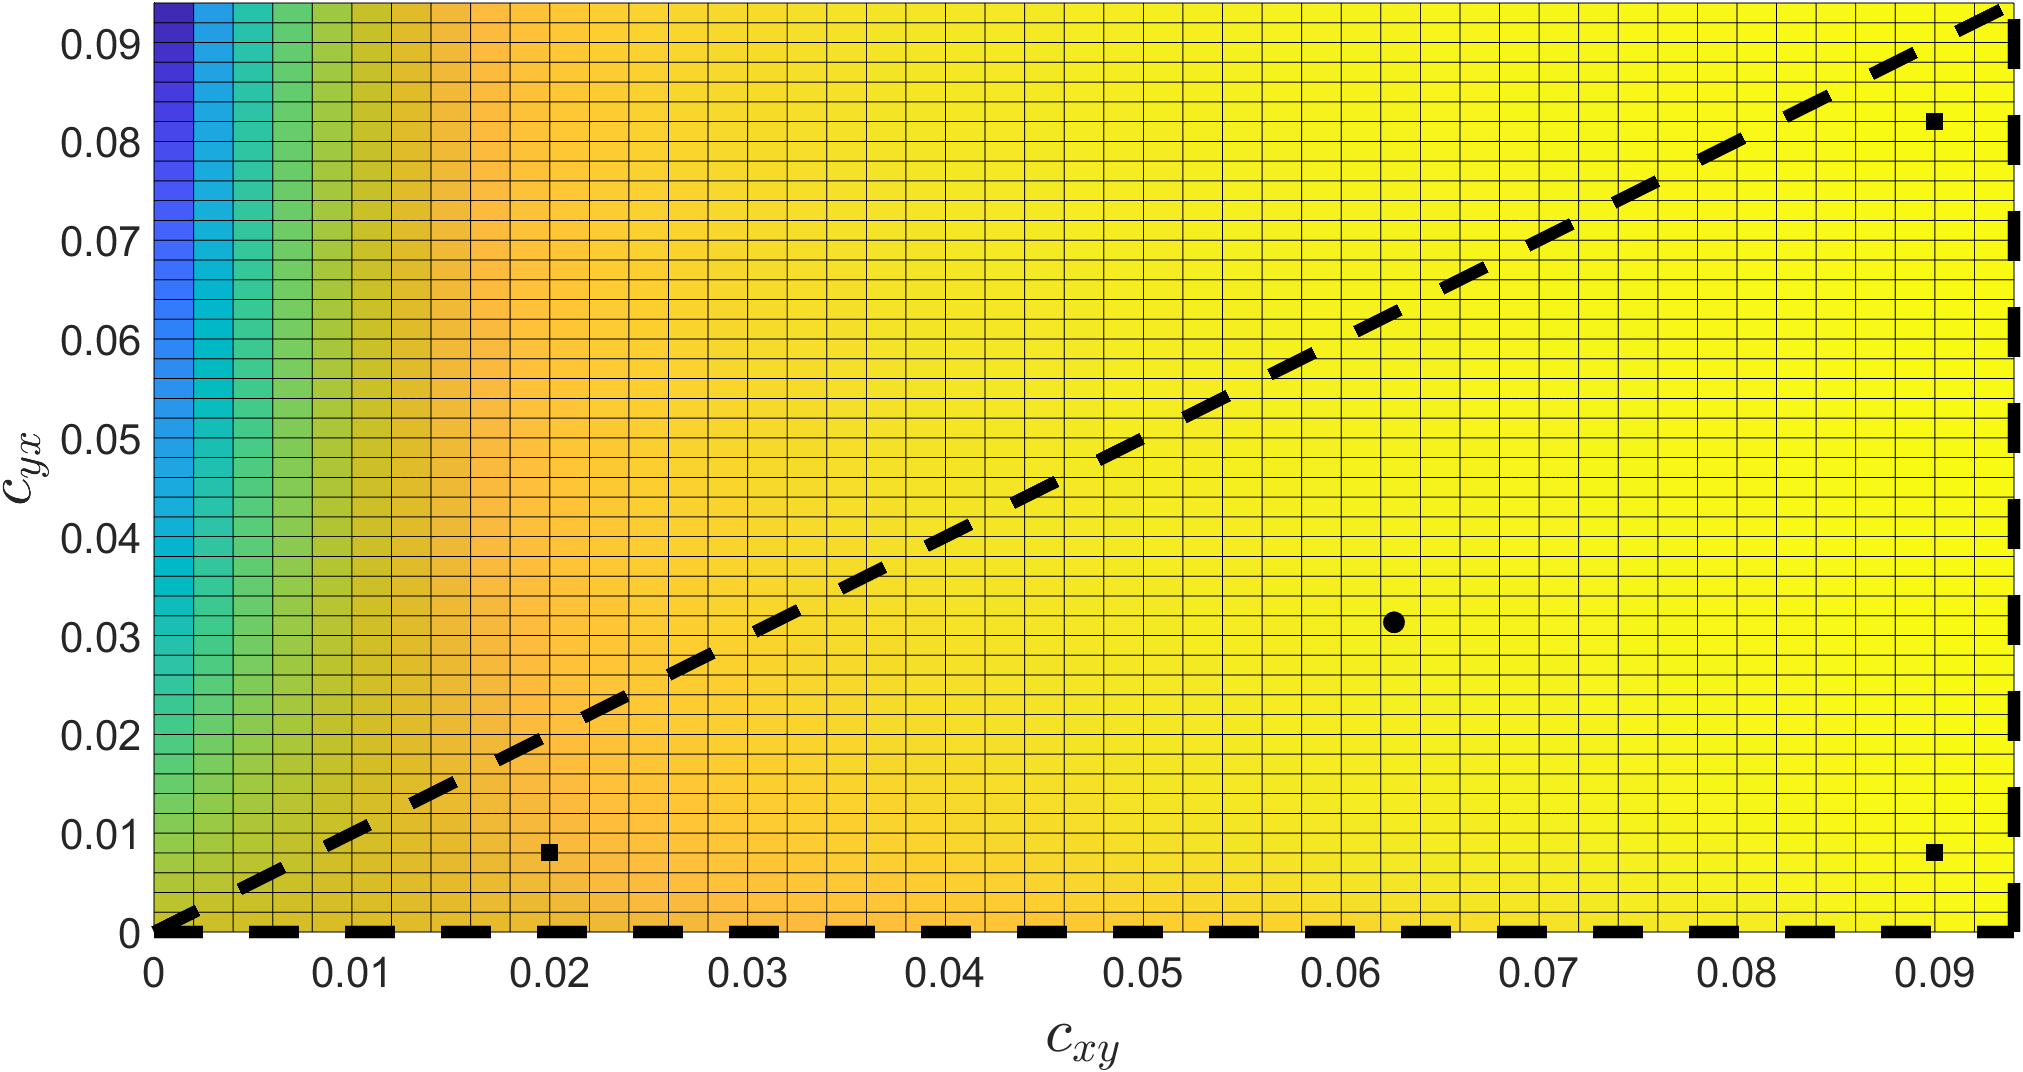
\includegraphics[width=14cm]{Pictures/Stability/TraceTopDown.png}
% \end{figure}
% \begin{figure}[H]
%     \centering
%     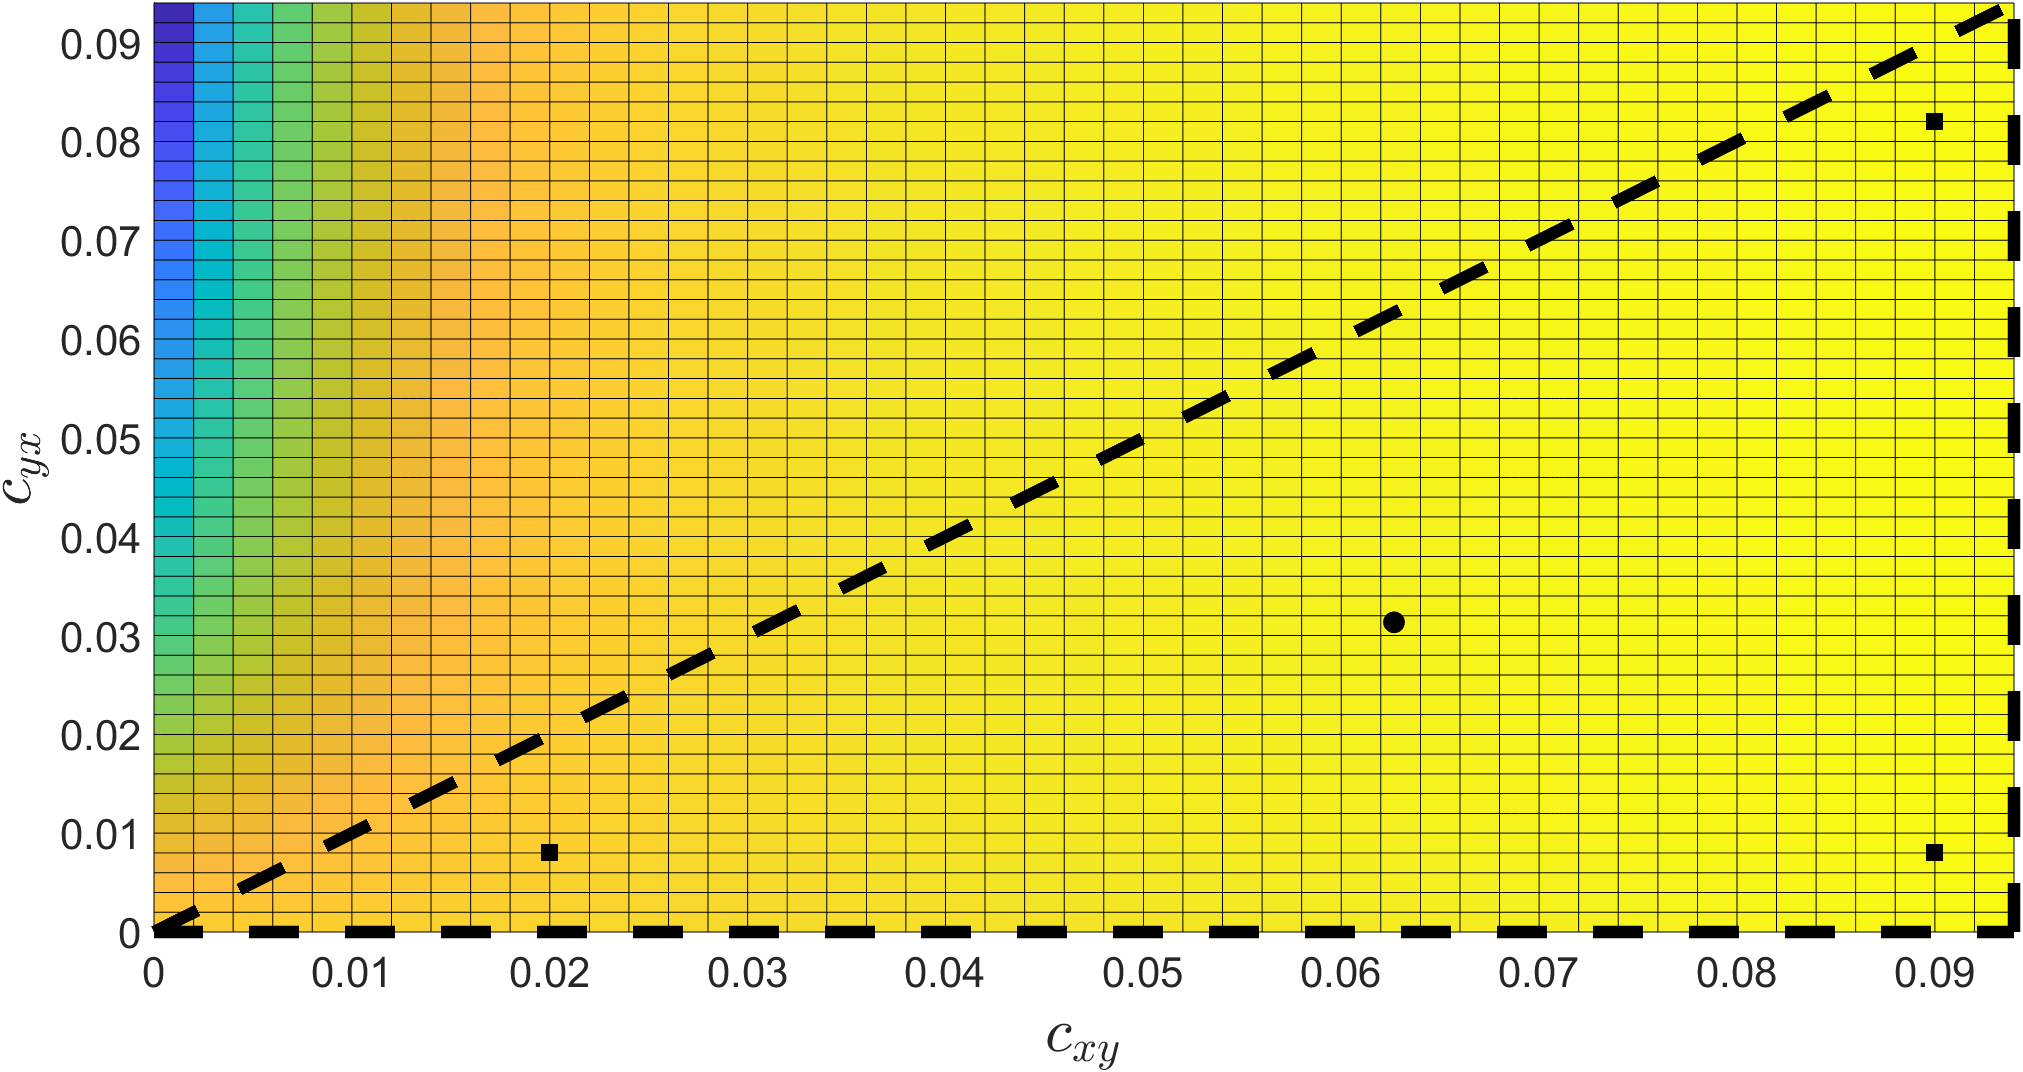
\includegraphics[width=14cm]{Pictures/Stability/DiscriminantTopDown.png}
%     \caption{Top-down view of \figureautorefname~\eqref{fig:TraceDiscriminant}. The points inside the right triangle are all values that satisfy the constraints of parameters $c_{yx}$ and $c_{xy}$. The right triangle's center of mass is marked with a black dot at the coordinate point $(0.0627,0.0313)$.}
%     \label{fig:TraceDiscriminantTopDown}
% \end{figure}
% In the figure above a region is drawn where all $c_{yx}$ and $c_{xy}$ satisfy their constraints.
% Now, testing different $c_{yx}$ and $c_{xy}$ values will illustrate how different interaction rates will effect the outcome of the each species' population.
% The values chosen for $(c_{xy},\;c_{yx})$ are $(0.02,\;0.008)$, $(0.09,\;0.008)$, $(0.09,\;0.082)$, and $(0.0627,\;0.0313)$. These pair of interaction parameters can be seen plotted on the figure above.
% To compare each of the parameters, we plot the solutions to \equationautorefname~\eqref{eq:AutonomousSystemODEs}, where the brown bear population is along the y-axis and the salmon population is along the x-axis as shown below for each pair of parameters.
% \begin{figure}[H]
%     \centering
%     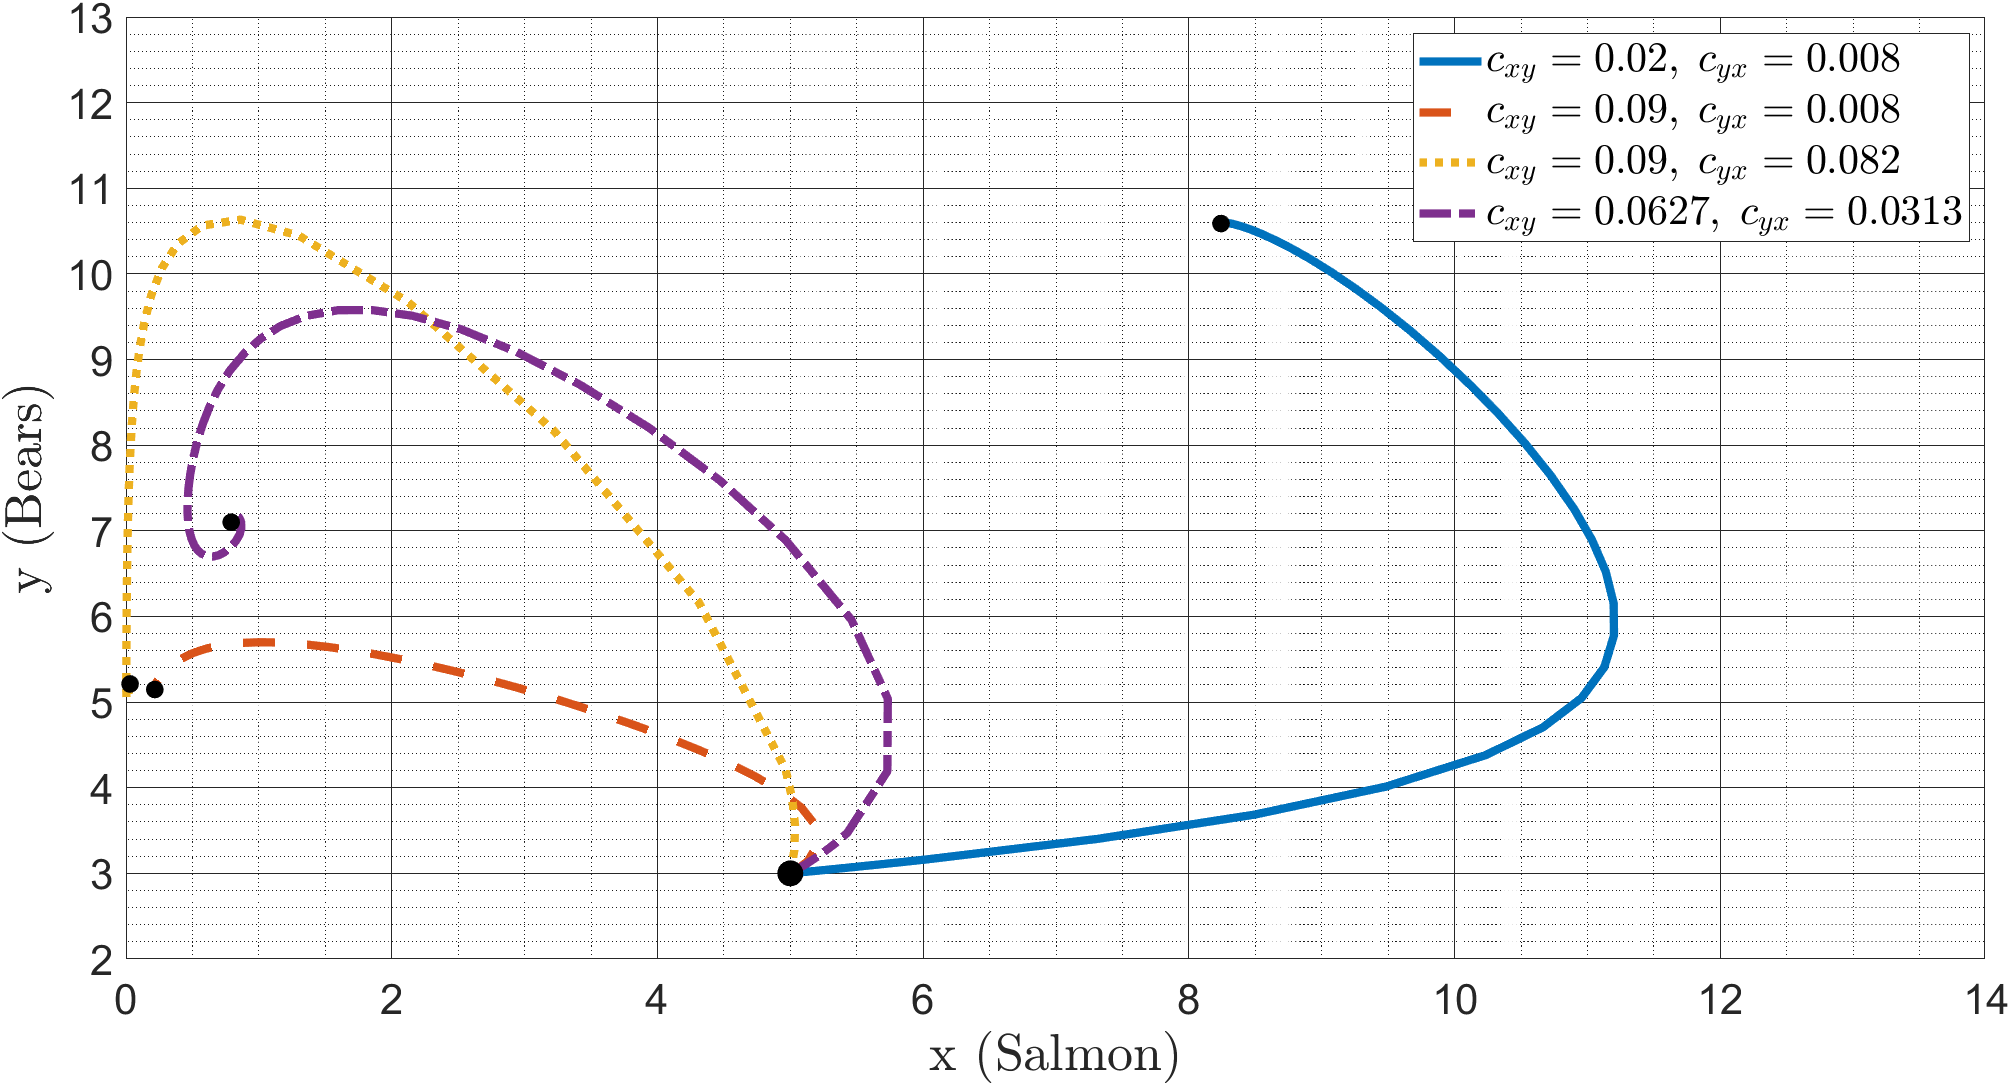
\includegraphics[width=14cm]{Pictures/Stability/SolutionsAutonomousModel.png}
%     \caption{Compares the effect of different interaction rates on the autonomous model, \equationautorefname~\eqref{eq:AutonomousSystemODEs}, where the initial conditions are $x_0 = 5$ and $y_0 = 3$.}
%     \label{fig:SolutionsAutonomous}
% \end{figure}
% The graph above shows that each of these parameters effects the location of the critical point, $(x^*_4,y^*_4)$ as well as the oscillations of the populations.
% We chose the initial conditions, $x_0 = 5$ and $y_0 = 3$, to illustrate the dramatic difference in interaction parameters.
% When $c_{xy}$ is large, the salmon population dies off, and when $c_{yx}$ is large, the brown bear population increases faster before converging near its carrying capacity.
% Lastly, when the pair of parameters is equal to the right triangle's center of mass in \figureautorefname~\ref{fig:TraceDiscriminantTopDown}, the population oscillates and converges to its critical point $(0.61,7.19)$.
% We will be using $c_{xy}=0.0627$ and $c_{yx}=0.0313$ to represent the interaction rates of the two species for \equationautorefname~\eqref{eq:AutonomousSystemODEs} because with these parameters the populations oscillate similar to what is expected in the real world.
% So, with all the parameters selected, the solutions to the autonomous model, \equationautorefname~\eqref{eq:AutonomousSystemODEs}, with respect time is shown below.
% \begin{figure}[H]
%     \centering
%     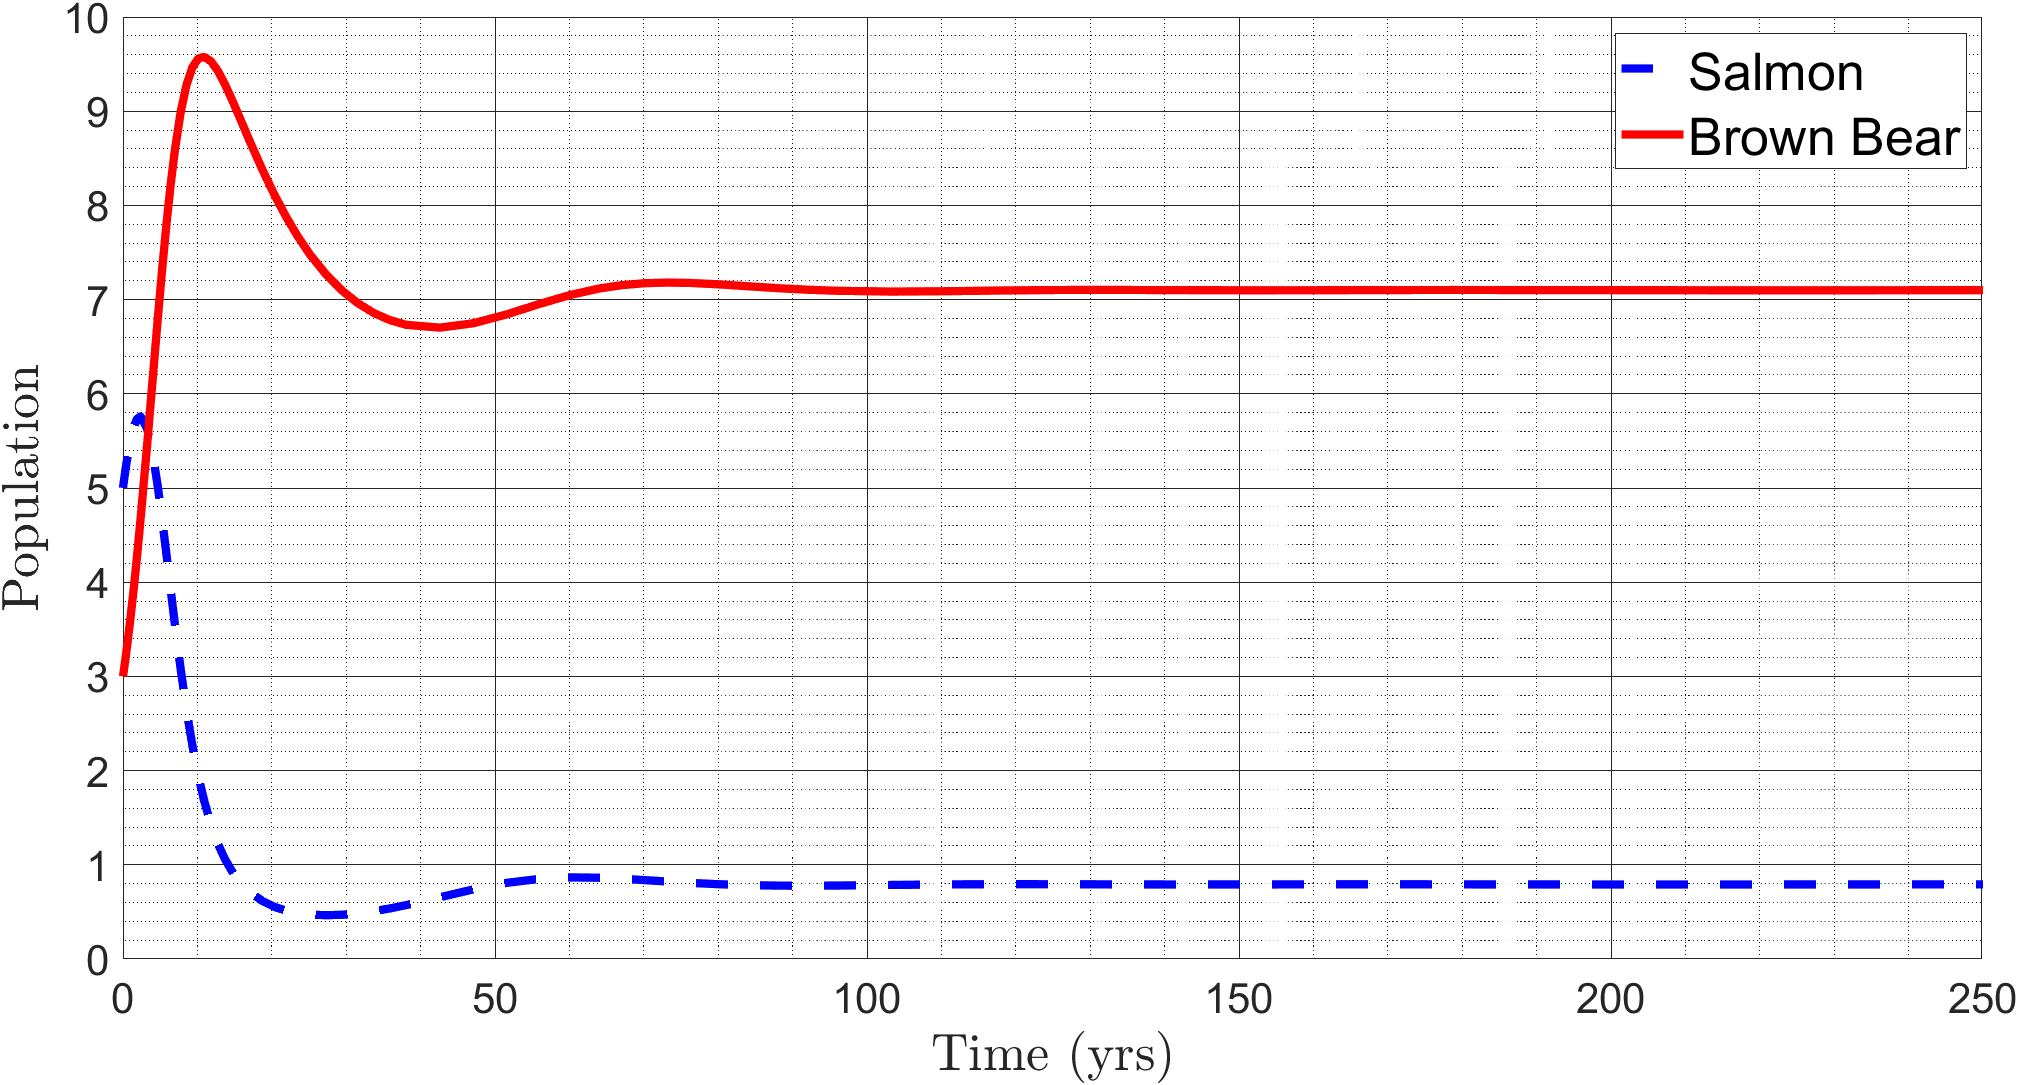
\includegraphics[width=14cm]{Pictures/System ODEs/AutonomousModelRespectTime.png}
%     \caption{Plot of  the solutions to the autonomous model, \equationautorefname~\eqref{eq:AutonomousSystemODEs}, with respect to time.}
%     \label{fig:SolutionsNonAutonomous}
% \end{figure}
% In the figure above, both populations briefly increase before changing directions and oscillating toward their equilibrium points.
% Based on this figure, the brown bear population will quickly overtake the salmon population, forcing the salmon near regional extinction.



% Now, we can compare these results to the system of ODEs, with the proposed growth rate, $G(t)$, shown below.
% \begin{equation}\label{eq:Non-AutonomousSystemODEs}
%     \begin{aligned}
%     \frac{dx}{dt} &=G(t)x\left(1-\frac{x}{K_x}\right) - c_{xy}xy,\\[.4cm]
%     \frac{dy}{dt} &=r_yy\left(1-\frac{y}{K_y}\right) + c_{yx}xy.
%     \end{aligned}
% \end{equation}
% Now, using the same parameters for the autonomous model, \equationautorefname~\eqref{eq:AutonomousSystemODEs}, we compare different initial conditions to analyze the stability of the model.
% \begin{figure}[H]
%     \centering
%     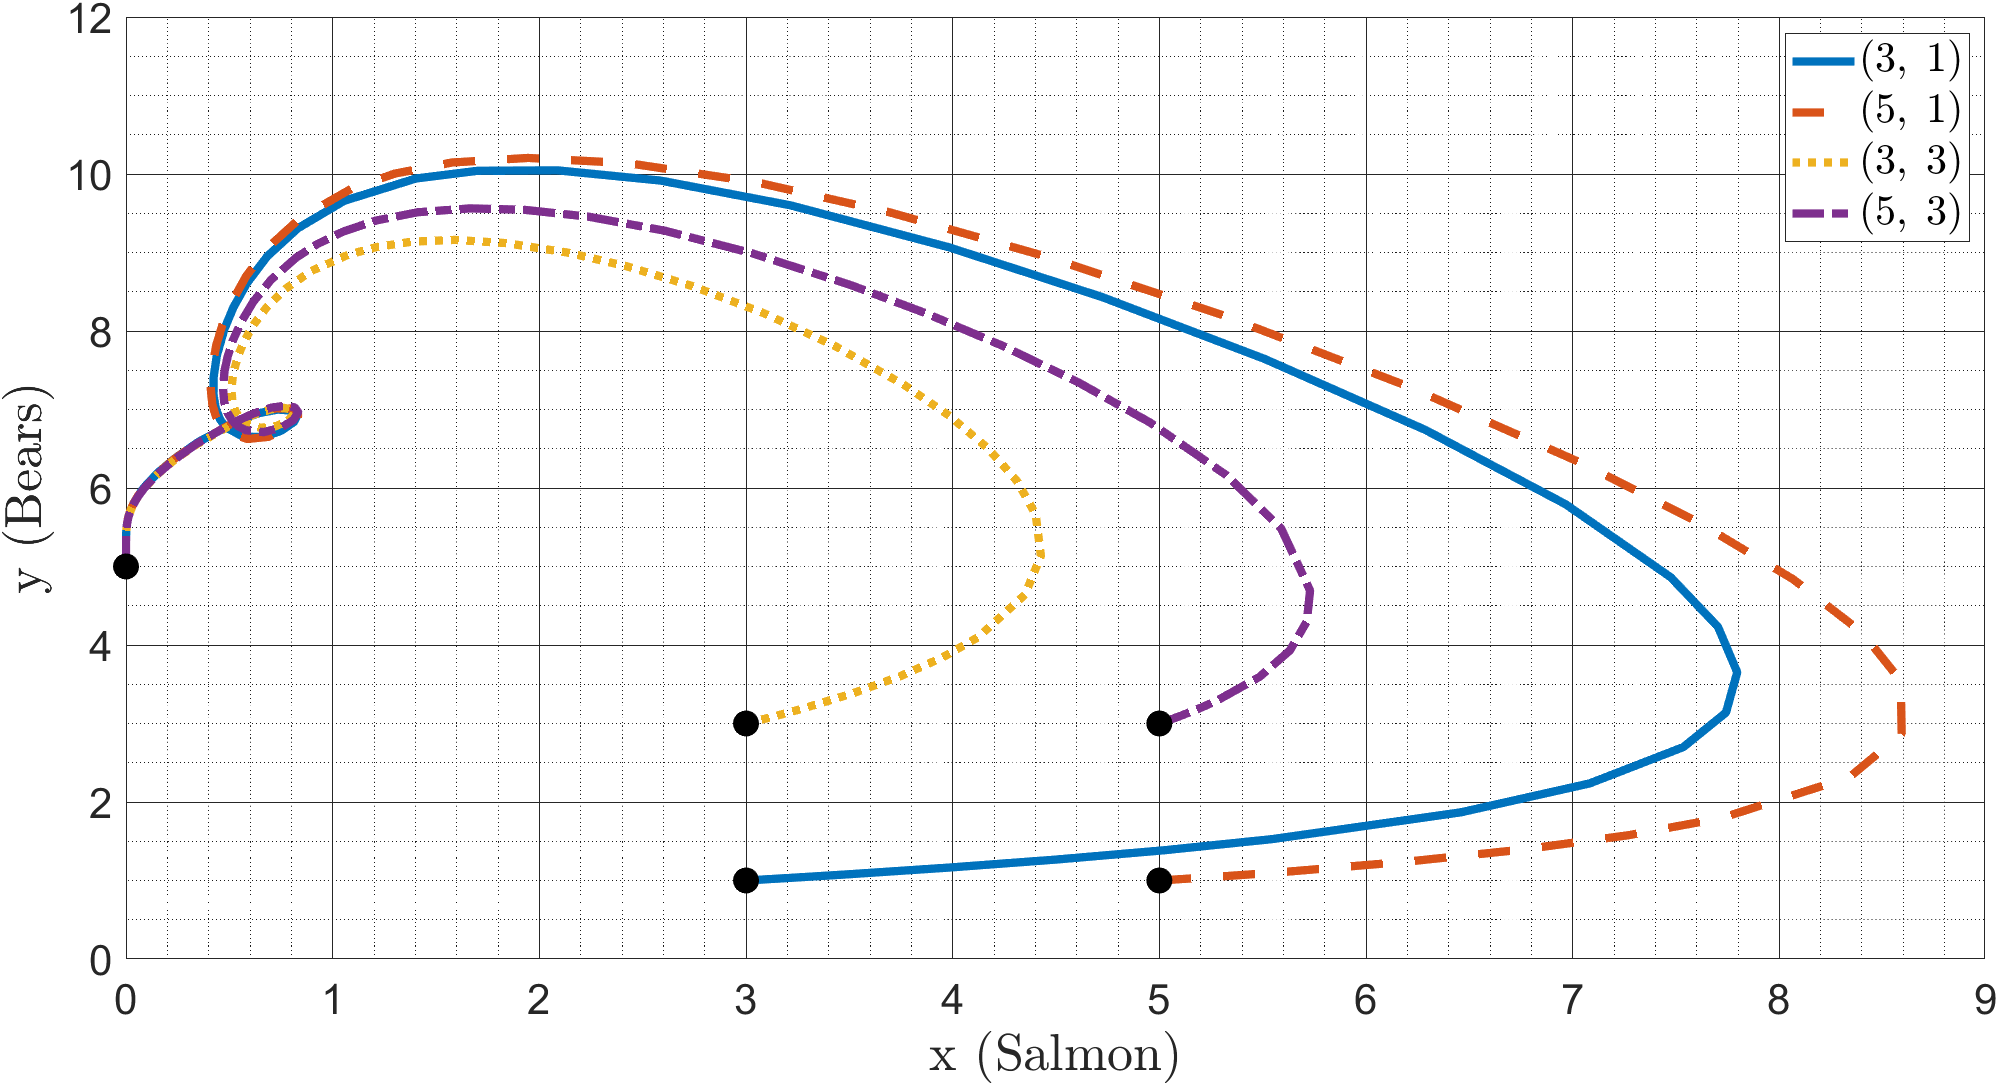
\includegraphics[width=14cm]{Pictures/Stability/SolutionsNonAutonomousModel.png}
%     \caption{Compares the solutions to the non-autonomous model, \equationautorefname~\eqref{eq:Non-AutonomousSystemODEs}, with different initial conditions.}
%     \label{fig:Non-AutonomousSystemODEs}
% \end{figure}
% As expected the salmon population converges to zero as seen in \figureautorefname~\eqref{fig:SalmonWithRepoFun}, resulting in the brown bear population converging to their carry capacity.
% When the salmon population dies off, the interaction terms in the model will approach zero and eventually the behavior of the brown bear species will be represented by its logistic equation, \equationautorefname~\eqref{eq:LogBear}.
% Lastly, in the graph below, we compare the results to the autonomous and non-autonomous model.
% \begin{figure}[H]
%     \centering
%     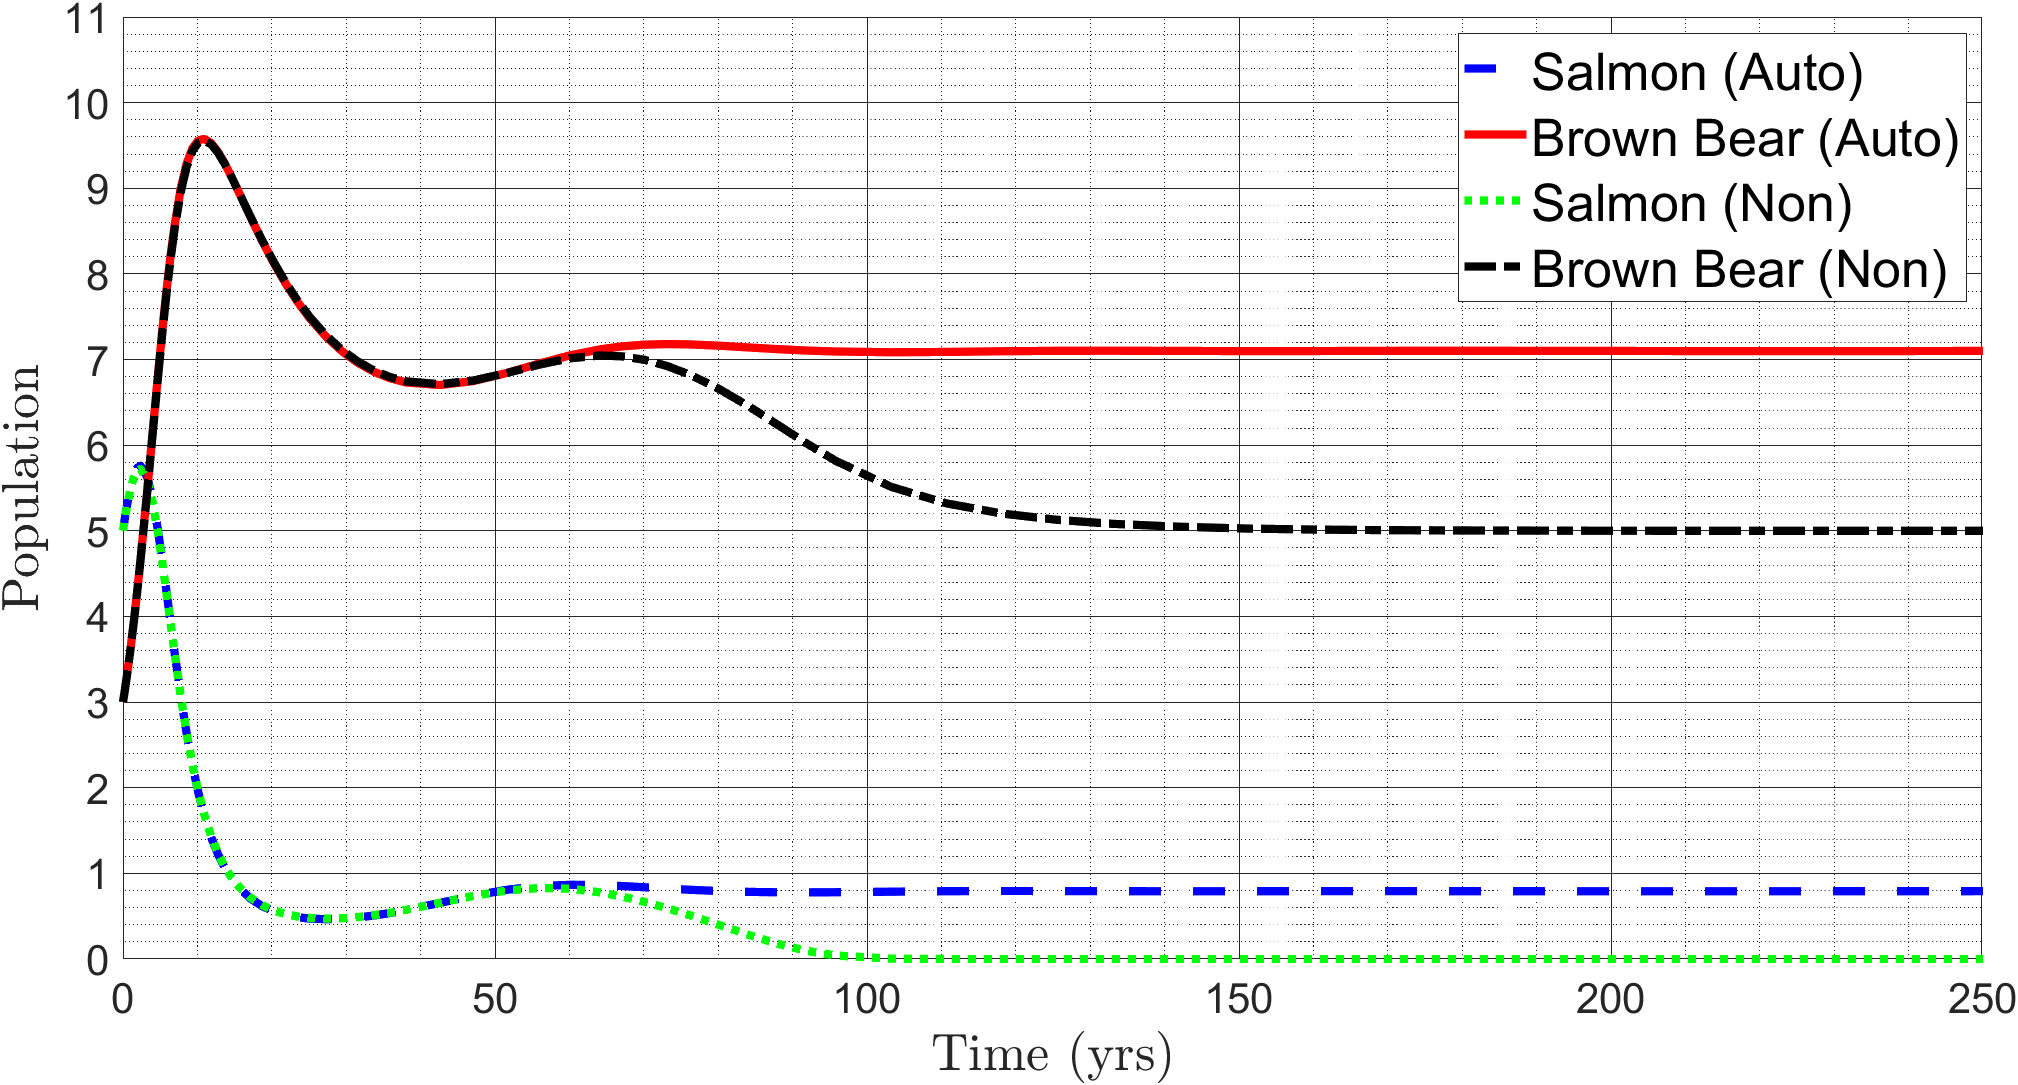
\includegraphics[width=14cm]{Pictures/System ODEs/AutonomousVsNonautonomous.png}
%     \caption{Plot of the solutions to the autonomous and non-autonomous model with respect to time.}
%     \label{fig:AutonomousVsNon-Autonomous}
% \end{figure}
% Initially, the two models follow the same path, but after approximately 65 years, the curves begin to deviate.
% According to our temperature function, \equationautorefname~\eqref{eq:sstmodel}, the projected Alaskan river temperature in 65 years is $T(65)\approx14.7^{\circ}$C.
% Therefore, the graph illustrates that soon after the river temperature leaves the optimal range, the difference in the outcomes of the species' populations becomes prominent.
% The non-autonomous model shows similar trends to the autonomous model, but ultimately resulting in the salmon population dying off and the Alaskan brown bear population converging to its carrying capacity.










% \begin{equation*}\scalebox{1.4}{$
%     \begin{array}{cc}
%          x^*_4 = \frac{\ln(R(T))*\frac{r_y}{K_y} - c_{xy}*r_y}{c_{xy}*c_{yx}+\frac{\ln{(R(T))}*r_y}{K_x*K_y}} & y^*_4 = \frac{\ln(R(T))*c_{yx}+\frac{\ln(R(T))}{K_x}*r_y}{c_{xy}*c_{yx}+\frac{\ln{(R(T))}*r_y}{K_x*K_y}} 
%     \end{array}$}
% \end{equation*}

\section{Non-Autonomous System of ODEs}

Now, we can compare the results from the previous section to a non-autonomous system of ODEs, where the growth rate is a function of time, shown below.
\begin{equation}\label{eq:Non-AutonomousSystemODEs}
    \begin{aligned}
    \frac{dx}{dt} &=G(t)x\left(1-\frac{x}{K_x}\right) - c_{xy}xy,\\[.4cm]
    \frac{dy}{dt} &=r_yy\left(1-\frac{y}{K_y}\right) + c_{yx}xy.
    \end{aligned}
\end{equation}
Now, using the same parameters for the autonomous model, \equationautorefname~\eqref{eq:AutonomousSystemODEs}, we consider the model with different initial conditions.
\begin{figure}[H]
    \centering
    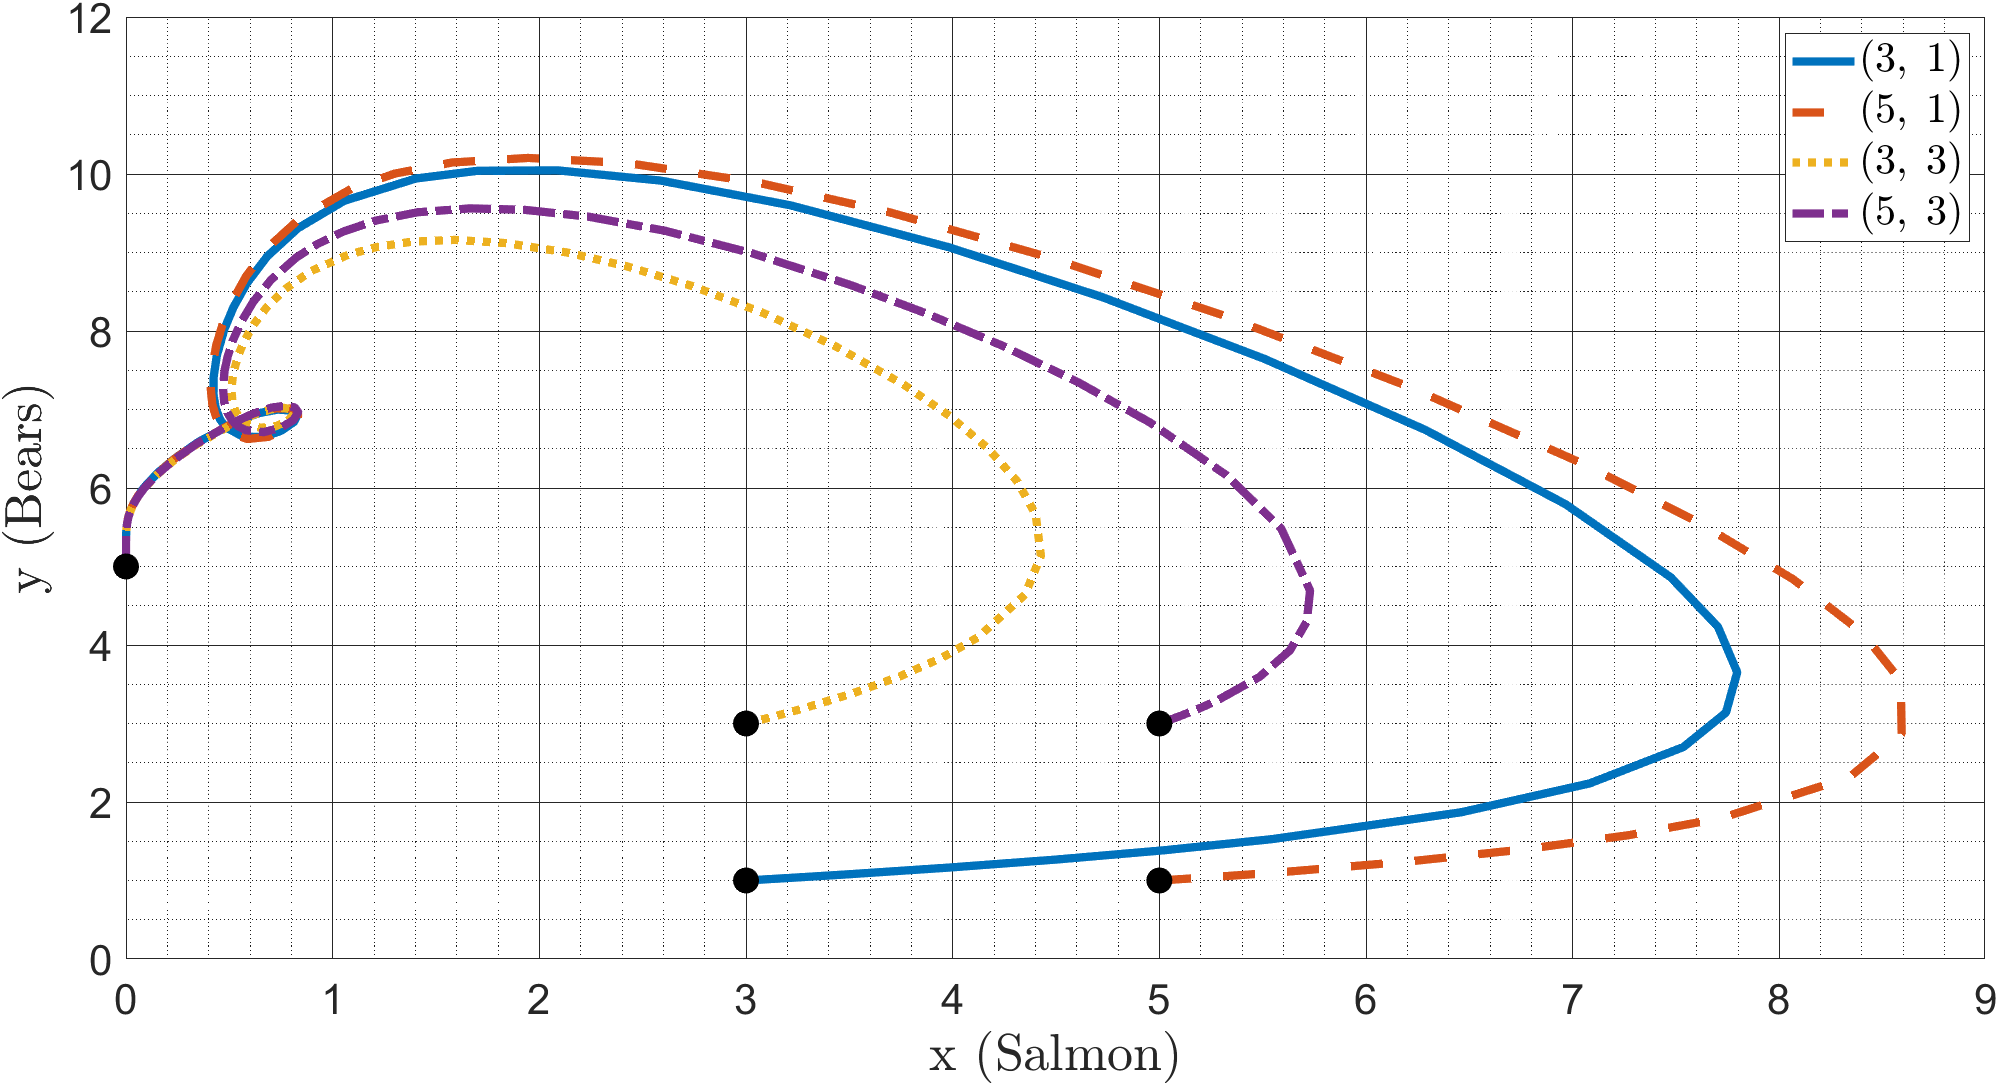
\includegraphics[width=14cm]{Pictures/Stability/SolutionsNonAutonomousModel.png}
    \caption{\singlespacing
    Compares the solutions to the non-autonomous model, \equationautorefname~\eqref{eq:Non-AutonomousSystemODEs}, with different initial conditions, $(x_0,\ y_0)$.}
    \label{fig:Non-AutonomousSystemODEs}
\end{figure}
As expected, the salmon population converges to zero as seen in \figureautorefname~\ref{fig:SalmonWithRepoFun}, resulting in the brown bear population converging to their carry capacity.
When the salmon population dies off, the interaction terms in the model will approach zero, and eventually, the behavior of the brown bear species will be represented by its logistic equation, \equationautorefname~\eqref{eq:LogBear}.
Lastly, in the graph below, we compare the results to the autonomous and non-autonomous models.
\begin{figure}[H]
    \centering
    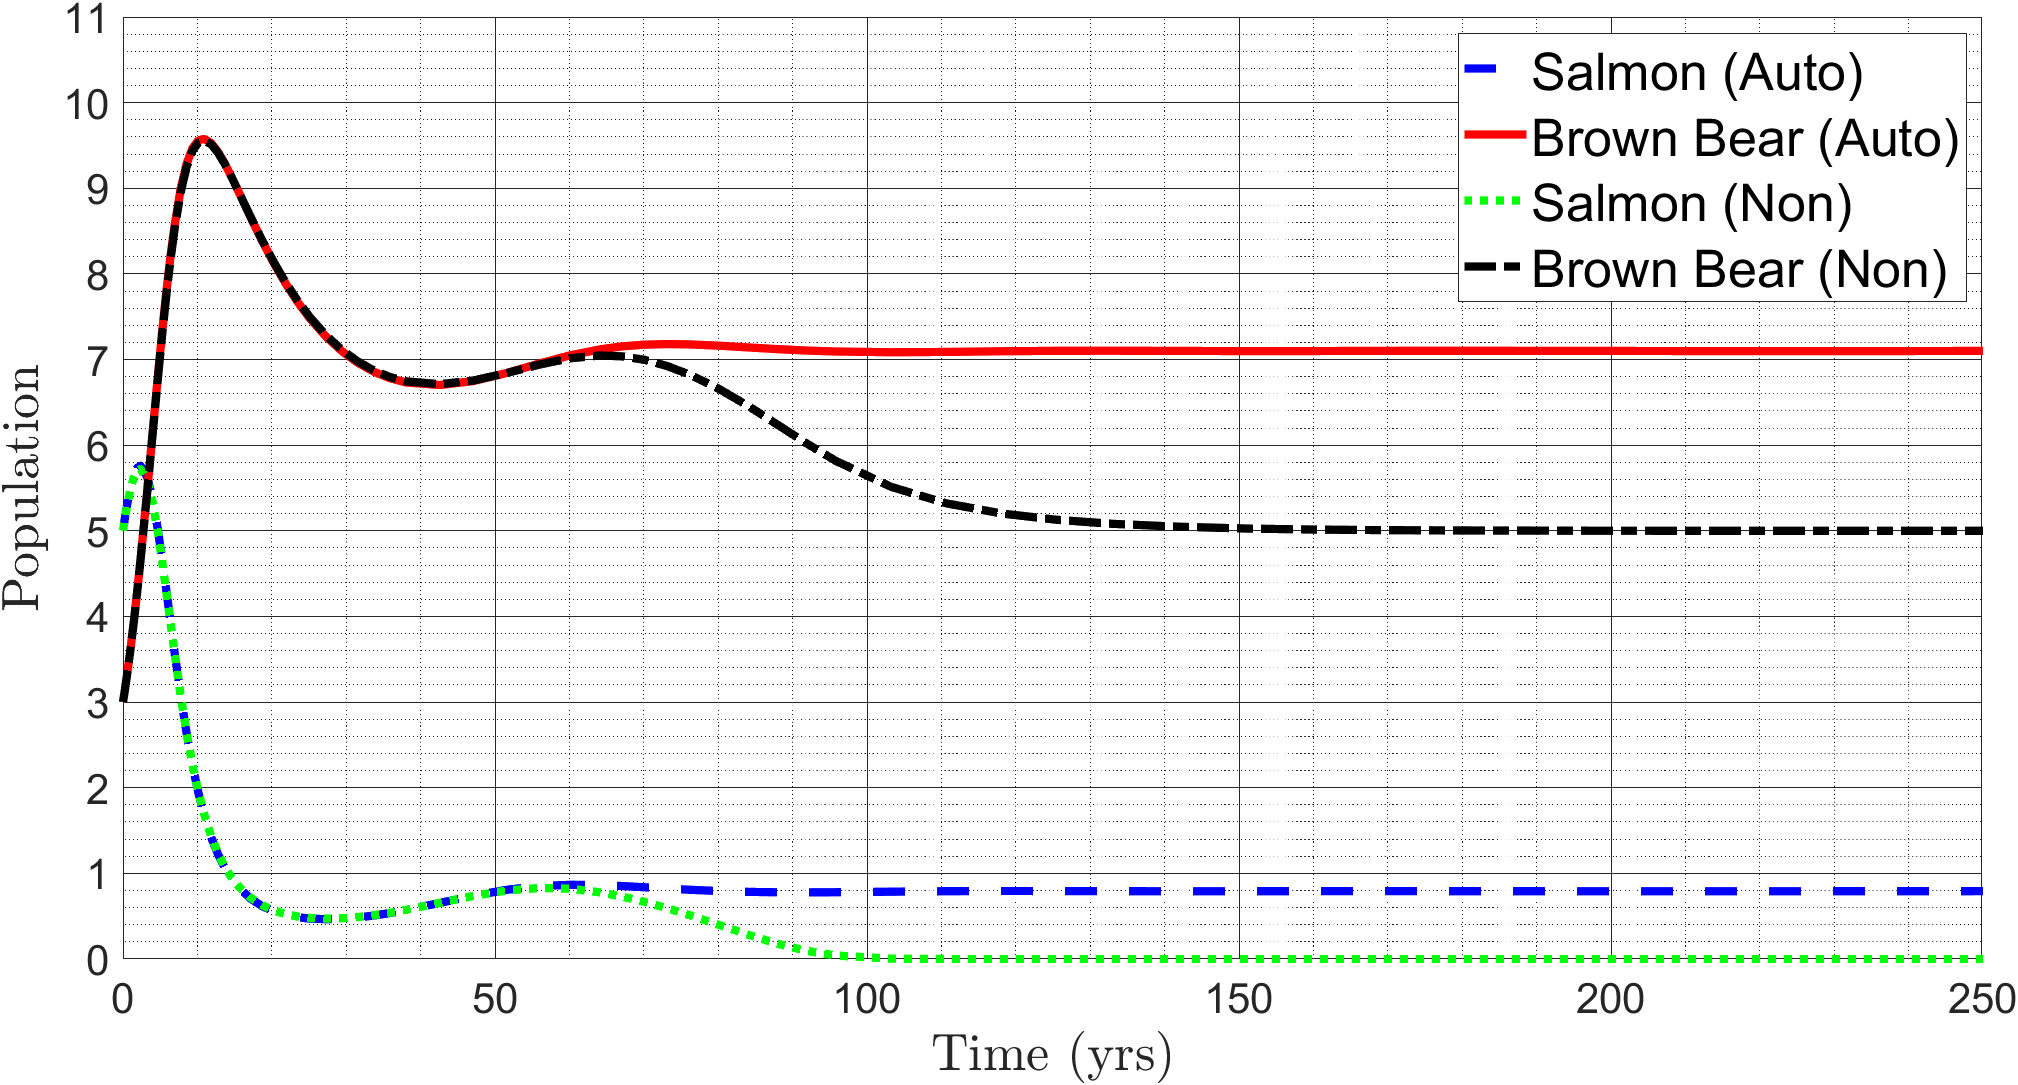
\includegraphics[width=14cm]{Pictures/System ODEs/AutonomousVsNonautonomous.png}
    \caption{\singlespacing
    Plot of the solutions to the autonomous and non-autonomous model with respect to time.}
    \label{fig:AutonomousVsNon-Autonomous}
\end{figure}
Initially, the two models follow the same path, but after approximately 60 years, the curves begin to deviate.
According to our temperature function, \equationautorefname~\eqref{eq:sstmodel}, the projected Alaskan river temperature in 60 years is $T(60)\approx14.34^{\circ}$C.
Therefore, the graph illustrates that soon after the river temperature leaves the optimal range, the difference in the outcomes of the species' populations becomes prominent.
The non-autonomous model shows similar trends to the autonomous model, but ultimately resulting in the salmon population dying off and the Alaskan brown bear population converging to its carrying capacity.












\section{Conclusion}

In this chapter, we proposed a salmon growth rate function that depends on water temperature.
We used river temperature data from the United States Geological Survey (USGS) to design a function that models the increase in Alaskan river temperature over time, which can be seen below,
\begin{equation*}
    T(t) = a*t + b,
\end{equation*}
where $a=0.08$, and $b=9.54$.
Also, $t=0$ represents the current year, 2022.
We then make the growth rate function dependent on time by replacing the temperature parameter $T$ with the temperature function, as shown bellow,
\begin{equation*}
    \begin{array}{ll}
        G(t) &= R(t) + \scalebox{1.2}{$\frac{P'(t)t}{P(t)}$} \\[.2cm]
         &= \ln\left(\scalebox{1.2}{$\frac{0.32*5}{1+10^{-4}(0.08t-2.96)^4}$}\right) - \scalebox{1.2}{$\frac{4*10^{-4}*0.08t(0.08t-2.96)^3}{1+10^{-4}(0.08t-2.96)^4}$}.
    \end{array}
\end{equation*}
Lastly, we replaced this new growth rate function with the growth rate parameter in the original logistic model, \equationautorefname~\eqref{eq:fishlogistic}, and compare its results.
We found that after approximately 100 years, the salmon population will begin to decline and eventually die off or migrate elsewhere.
In the next chapter, we will examine the effect of interaction between the brown bear and salmon species.
We will compare the results of the interaction with and without the growth rate function.

\chapter{Conclusion}

% In the first section of chapter 2, we introduced the discussion of climate change and reported predictions of future global temperatures.
% Researchers anticipate that the earth's surface temperature will increase an average of $3.2^{\circ}$C by the $22^{nd}$ century~\cite{raftery2017less}.
% In the remaining chapter sections, we reviewed the logistic growth,  Lotka-Volterra, and competitive predator-prey equations, which we use throughout the thesis to describe the interactive relationship between Alaskan brown bears and pacific salmon.

In chapter 2, we use the logistic growth model to simulate the population of both species, Alaskan brown bears and pacific salmon.
In the first section, we estimated the growth rate parameter, $r_x = \ln(0.32*5)$, for salmon using reports from the Alaskan Department of Fish and Game.
We estimated the salmon's carrying capacity, $K_x=29.1*10^6$ by calculating the maximum volume of salmon in Bristol Bay, Alaska, for any given inshore run.
In the second section, we approximate the growth rate parameter, $r_y=0.059$, for brown bears by taking the average of three growth rates reported in three articles.
Using information from the Alaskan Department of Fish and Game, we estimated a parameter value, $K_y=4.5*10^4$, for the carrying capacity of the brown bear species.
Ultimately, we found that after 14 years, the salmon population should reach its environmental capacity if they start with an initial population of 20 million, and the brown bears will reach their environmental capacity in approximately 100 years if they begin with an initial population of 30 thousand.

In the first section of chapter 3, we use data from Dr. Phyllis Weber Scannel and Katherine Carter to approximate the proportion of salmon who survive spawning migration at different temperatures.
We develop a survival proportion function dependent on temperature for migrating salmon by fitting a curve to our approximated survival proportions.
Combining this function with the growth rate parameter of salmon found in chapter 2, we propose a growth rate function dependent on temperature.
In the next section of chapter 3, we used river temperature data from the United States Geological Survey to design a function that models the increase in Alaskan river temperature over time.
Substituting the temperature equation for the temperature parameter in the growth rate function proposed in the first section changes the growth rate for salmon to a function of time.
We found that after 100 years, the water temperature for salmon will become too hot to survive spawning migration, resulting in their regional extinction.

In chapter 4, we introduce interaction terms to both species' logistic models using a variation of Theodore Modis' system of ordinary differential equations.
In the second section of chapter 4, we analyze different interaction parameters for the model when neither species is affected by climate change.
After testing different parameters, we chose $c_{xy} = 0.0627$ and $c_{yx} = 0.0313$ to represent the interaction between the species and evaluated the solutions to the autonomous system.
The solutions to the autonomous model showed that when neither species is affected by climate change, the brown bears will overtake the salmon, and both species will oscillate toward their equilibrium point, $(0.79,\;7.1)$.
In the third section, we incorporate climate change into the autonomous system by making the growth rate a function of time, creating a non-autonomous model.
Using the interaction parameters in the previous section,  we analyzed the behavior of both species by plotting the solutions to the non-autonomous model with different initial conditions.
When comparing the two models proposed in this chapter, we found that as the temperature begins to leave the optimal range, the solutions to the non-autonomous model separate from those of the autonomous one, forcing the entire salmon population to become regional extinct from Alaska, and the brown bear population converging to its carrying capacity.

Plenty of variations of our non-autonomous model can be implemented to improve its accuracy.
While the logistic growth equation is useful for modeling population growth, another is age-structure models.
With brown bears and salmon having different survival and reproduction rates at different ages, an age-structure model might be more effective for predicting their behaviors~\cite{daele2010management,palstra2009age}.
Another aspect of our model worth exploring is growth rate functions.
A limitation we faced in developing a growth rate function for the salmon species was the need for more research in determining survival rates for migrating salmon at different temperatures.
% Another growth rate function we considered using was
% \begin{equation*}
%     G(t) = r_x*P(t) - d,
% \end{equation*} 
% where $P(t)$ would represent the salmon survival proportions with respect to time, $r_x$ represents the growth rate parameter, and $d$ is the death rate for the pacific salmon.
Lastly, the Alaskan Department of Fish and Game reports that they adjust harvest rates periodically for brown bears to maintain their population size, so including a term to represent the change in harvest rates would significantly improve the accuracy of our model~\cite{daele2010management}.
We hope our model is used in further research to protect salmon and brown bears from the extreme weather that global warming will bring.

% ----------------------------------------------------------------------------- %

% BIBLIOGRAPHY
 
% The \SuppChap command should be issued before the bibliography to update
% the display style in the Table of Contents
\SuppChap

\newpage
 
%\begin{thebibliography}{99}
%
%\bibitem{Lamport} 
%Leslie Lamport,
%\textit{\LaTeX: A Document Preparation System},
%Addison-Wesley Professional,
%2nd Edition,
%1994
%
%\end{thebibliography}
\bibliographystyle{ieeetr}
\urlstyle{same}
\bibliography{CitationsBrownBears.bib}
\addcontentsline{toc}{chapter}{{Bibliography}}

\clearpage

% ----------------------------------------------------------------------------- %

% APPENDICES

% The \AddAppendix command should be issued before the first appendix to update
% the display style in the Table of Contents
\AddAppendix

\appendix

\chapter{TABLES}\label{appendix:salmon}

\newpage
\begin{center}
    \rowcolors{2}{white!40}{lightgray!40}
    \LTcapwidth=\textwidth
    \begin{longtable}[c]{|P{2cm}|P{3cm}|P{3cm}|}

    \caption{Sockeye Comparison Between Weight and Run Size in Bristol Bay}\label{tab:runvsweight}\\
    
    \hline 
    \rowcolor{white!40}\textbf{Year} & \textbf{Weight (lbs)} & \textbf{Run (mil)}\\ 
    \hline
    \endfirsthead
    
    \rowcolor{lightgray!40}    
    \multicolumn{3}{c}{{\bfseries \tablename\ \thetable{} -- continued from previous page}} \\
    \hline \rowcolor{white!40} \textbf{Year} & \textbf{Weight (lbs)} & \textbf{Run} \\ \hline 
    \endhead

    \hline \multicolumn{3}{|r|}{{\textbf{Continued on next page}}} \\ \hline
\endfoot

\hline \hline
\endlastfoot
    
         2001 & 6.7 & 22.3\\
         2002 & 6.1 & 16.9\\
         2003 & 6.3 & 24.9\\
         2004 & 5.8 & 41.9\\
         2005 & 6.3 & 39.3\\
         2006 & 5.7 & 42.9\\
         2007 & 5.8 & 44.8\\
         2008 & 5.8 & 40.4\\
         2009 & 5.9 & 40.4\\
         2010 & 5.5 & 40.6\\
         2011 & 6.2 & 30.6\\
         2012 & 5.7 & 30.4\\
         2013 & 6.0 & 24.4\\
         2014 & 5.6 & 41.1\\
         2015 & 5.2 & 58.8\\
         2016 & 5.4 & 51.7\\
         2017 & 5.5 & 57.6\\
         2018 & 5.1 & 63.0\\
         2019 & 5.1 & 56.4\\
         2020 & 5.1 & 58.3\\
         2021 & 4.7 & 67.7\\
         \hline
    \end{longtable}
    \vspace{1ex}
    
    {\singlespacing
    % \raggedright 
    *Comparing the average weight of sockeye salmon to their run size in Bristol Bay each year. 
    The data used to make this table was taken from the ``\emph{2021 BRISTOL BAY AREA ANNUAL MANAGEMENT REPORT}''~\cite{bristol}.\par}
\end{center}
\vspace{2cm}

\begin{center}
    
    \rowcolors{2}{white!40}{lightgray!40}
    \LTcapwidth=\textwidth
    \begin{longtable}[c]{|P{4.1cm}|P{4.1cm}|}

    \caption{Volume of Sockeye Salmon Runs Each Year in Bristol Bay}\label{tab:volume}\\
    
    \hline 
    \rowcolor{white!40}\textbf{Year} & \textbf{Volume (MMCF)}\\ 
    \hline
    \endfirsthead
    
    \rowcolor{lightgray!40}    
    \multicolumn{2}{c}{{\bfseries \tablename\ \thetable{} -- continued from previous page}} \\
    \hline \rowcolor{white!40} \textbf{Year} & \textbf{Volume (MMCF)} \\ \hline 
    \endhead

    \hline \multicolumn{2}{|r|}{{\textbf{Continued on next page}}} \\ \hline
\endfoot

\hline \hline
\endlastfoot
    
        2001 & 3.41 \\
        2002 & 2.35 \\
        2003 & 3.58 \\
        2004 & 5.55 \\
        2005 & 5.65 \\
        2006 & 5.58 \\
        2007 & 5.93 \\
        2008 & 5.35 \\
        2009 & 5.44 \\
        2010 & 5.1 \\
        2011 & 4.33 \\
        2012 & 3.96 \\
        2013 & 3.34 \\
        2014 & 5.25 \\
        2015 & 6.98 \\
        2016 & 6.37 \\
        2017 & 7.23 \\
        2018 & 7.34 \\
        2019 & 6.57 \\
        2020 & 6.79 \\
        2021 & 7.26 \\
         \hline
         \nopagebreak
    \end{longtable}
    \vspace{1ex}
    
    {\singlespacing
    % \raggedright 
    *Using \tablename~\ref{tab:runvsweight} to calculate the volume for each year.\par}
\end{center}
\vspace{2cm}
\begin{table}[H]
\rowcolors{2}{white!40}{lightgray!40}
    \centering
    \caption{Average Annual Harvest For Salmon in Bristol Bay}\label{tab:harvestBristol}
    \vspace{.25cm}
    \begin{tabular}{|c|c|}
    \hline
         \textbf{Species} & \textbf{Harvest} \\
         \hline
         Sockeye & 28,100,000\\
         Chinook & 39,571\\
         Chum & 1,100,000\\
         Coho & 95,583\\
         Pink & 510,000\\
         \hline
         \textbf{\color{black}Total} & \textbf{29,845,154}\\
         \hline
    \end{tabular}
    \vspace{1ex}
    
    {\singlespacing
    % \raggedright 
    *Average annual commercial harvest for each salmon species from $(2001 - 2020)$~\cite{bristol}. Pink Salmon are reported in even years because of their two-year life cycle pattern.\par}
\end{table}

\chapter{R Code}\label{appendix:RCode}

\definecolor{codegreen}{rgb}{0,0.6,0}
\definecolor{codegray}{rgb}{0.5,0.5,0.5}
\definecolor{codepurple}{rgb}{0.58,0,0.82}
\definecolor{backcolour}{rgb}{0.95,0.95,0.92}
\definecolor{codeblue}{rgb}{0,0.33,1}
\definecolor{codeorange}{rgb}{1,0.5,0}

\lstdefinestyle{mystyle}{
    backgroundcolor=\color{white},   
    commentstyle=\color{codegreen},
    keywordstyle=\color{codeblue},
    numberstyle=\tiny\color{codegray},
    stringstyle=\color{codeorange},
    basicstyle=\ttfamily\footnotesize,
    breakatwhitespace=false,         
    breaklines=true,                 
    captionpos=b,                    
    keepspaces=true,                 
    numbers=left,                    
    numbersep=5pt,                  
    showspaces=false,                
    showstringspaces=false,
    showtabs=false,                  
    tabsize=2
}

\lstset{style=mystyle}

\section{Salmon Run Size Vs Their Average Weight}

\lstinputlisting[language=r]{Code/R/runVSweight.R}


\section{Proportion Function}

\lstinputlisting[language=r]{Code/R/Proportion Model.R}


\section{Water Temperature Dependent on Time}

\subsection{Polynomial Fit of Surface Temperature}

\lstinputlisting[language=r]{Code/R/Global Temp - NOAA.R}

\subsection{Polynomial Fit of Sea Surface Temperature}

\lstinputlisting[language=r]{Code/R/Global SST - NOAA.R}

\subsection{Linear Fit}

\lstinputlisting[language=r]{Code/R/Alaska Water Temp.R}


\chapter{MATLAB Code}\label{appendix:MatlabCode}

\definecolor{codegreen}{rgb}{0,0.6,0}
\definecolor{codegray}{rgb}{0.5,0.5,0.5}
\definecolor{codepurple}{rgb}{0.58,0,0.82}
\definecolor{backcolour}{rgb}{0.95,0.95,0.92}
\definecolor{codeblue}{rgb}{0,0.33,1}
\definecolor{codeorange}{rgb}{1,0.5,0}

\lstdefinestyle{mystyle}{
    backgroundcolor=\color{white},   
    commentstyle=\color{codegreen},
    keywordstyle=\color{codeblue},
    numberstyle=\tiny\color{codegray},
    stringstyle=\color{codeorange},
    basicstyle=\ttfamily\footnotesize,
    breakatwhitespace=false,         
    breaklines=true,                 
    captionpos=b,                    
    keepspaces=true,                 
    numbers=left,                    
    numbersep=5pt,                  
    showspaces=false,                
    showstringspaces=false,
    showtabs=false,                  
    tabsize=2
}

\lstset{style=mystyle}

\section{Ordinary Differential Equation}

% \subsection{Logistic Equation as a Function of x}

% \lstinputlisting[language=matlab]{Code/MATLAB/LogODE.m}

\subsection{Salmon Exponential Equation}

\lstinputlisting[language=matlab]{Code/MATLAB/SalmonGrowthRate.m}

\subsection{Salmon Logistic Equation}

\lstinputlisting[language=matlab]{Code/MATLAB/SalmonLogisticGrowth.m}

\subsection{Brown Bear Logistic Equation}

\lstinputlisting[language=matlab]{Code/MATLAB/BrownBearPop.m}

\section{Growth Rate Function}

\subsection{Growth Rate Function Dependent on Time}

\lstinputlisting[language=matlab]{Code/MATLAB/SalmonRepoFunctionLogged.m}

\subsection{Salmon Model with Growth Rate Function}

\lstinputlisting[language=matlab]{Code/MATLAB/SalmonPopulationModelwithReproduction.m}

\section{Interaction Term Parameters}

\subsection{The Jacobian Matrix}

\lstinputlisting[language=matlab]{Code/MATLAB/JacobianTheModel.m}

\subsection{Trace and Discriminant}

\lstinputlisting[language=matlab]{Code/MATLAB/StabilityofTheModel.m}

\subsection{Autonomous Model with Different Parameters}

\lstinputlisting[language=matlab]{Code/MATLAB/TheModelParameters.m}

\section{The System of ODEs Model}

\subsection{The Autonomous Model}

\lstinputlisting[language=matlab]{Code/MATLAB/TheModel.m}

\subsection{The Non-Autonomous Model}

\lstinputlisting[language=matlab]{Code/MATLAB/TheModelReproductionFunction.m}

\subsection{Comparing Autonomous Vs Non-Autonomous}

\lstinputlisting[language=matlab]{Code/MATLAB/AutonomousVSNonAutonomous.m}






% ----------------------------------------------------------------------------- %

\end{document}


